\documentclass{article}
\usepackage[utf8]{inputenc}
\usepackage{longtable}
\usepackage{makecell}
\usepackage{geometry}
\usepackage{hyperref}
\usepackage{rotating}
\usepackage{tablefootnote}
\usepackage{float}
\usepackage{caption}
\usepackage{graphicx}
\usepackage{framed,enumitem}
%\usepackage{vrsion}

\usepackage{multicol}

\restylefloat{table}


% initialize some colors and highlighting that we will use throughout

\usepackage{xcolor} 
\usepackage{soul}

\definecolor{ELENcol}{RGB}{145,141,136}
\definecolor{ELLIcol}{RGB}{200,195,117}
\definecolor{ELDIcol}{RGB}{228,221,205 }
\definecolor{PARLcol}{RGB}{255,202,203}
\definecolor{PAREcol}{RGB}{227,213,236}
\definecolor{RESEcol}{RGB}{203,239,251}
\definecolor{POLIcol}{RGB}{204,226,240}
\definecolor{MEMEcol}{RGB}{203,239,221}
\definecolor{PARTcol}{RGB}{255,254,206}
\definecolor{FACTcol}{RGB}{255,242,203}
\definecolor{COMMcol}{RGB}{244,170,66}
\definecolor{QUOTcol}{RGB}{203,253,47}

\newcommand{\specialcell}[2][c]{%
  \begin{tabular}[#1]{@{}c@{}}#2\end{tabular}}

 \geometry{
 a4paper,
 total={170mm,257mm},
 left=20mm,
 top=20mm,
 }

\title{\gls{pcc} - Codebook V4.0.0}

\author{The \gls{pcc} project team}

\date{\today}

%glossary
% Load the package
\usepackage[nopostdot]{glossaries}
\makeglossaries

\begin{document}

\maketitle
%\version

%%%%%%%%%%%%%%%%%%%%%%%%%%
%generate glossary entries
%%%%%%%%%%%%%%%%%%%%%%%%%%
%actions
\newglossaryentry{comp}{name=COMP, description={Collect and follow-up until complete}}
\newglossaryentry{cwa}{name=CWA, description={Collect when available}} %note: should this be collect IF available?
\newglossaryentry{cwe}{name=CWE, description={Collect when easy}} %note: should this be collect IF easy?
\newglossaryentry{dnc}{name=DNC, description={Do Not Collect}}

%dataframe names
\newglossaryentry{pcc}{name=PCC, description={Parliamentary Careers in Comparison}}
\newglossaryentry{POLI}{name = POLI, description = {Politician Level Data Frame}}
\newglossaryentry{PARE}{name = PARE, description = {Parliamentary Episode Data Frame}}
\newglossaryentry{PARL}{name = PARL, description = {Parliament Data Frame}}
\newglossaryentry{MEME}{name = MEME, description = {Membership Episode Data Frame}}
\newglossaryentry{PART}{name = PART, description = {Party Data Frame}}
\newglossaryentry{FACT}{name = FACT, description = {Faction Data Frame}}
\newglossaryentry{COMM}{name = COMM, description = {Committee Data Frame}}
\newglossaryentry{ELLI}{name = ELLI, description = {Electoral List Data Frame}}
\newglossaryentry{ELEN}{name = ELEN, description = {Electoral List Entry Data Frame}}
\newglossaryentry{ELDI}{name = ELDI, description = {Electoral District Data Frame}}
\newglossaryentry{RESE}{name = RESE, description = {Resume Entries Data Frame}}
\newglossaryentry{ORGS}{name = ORGS, description = {Organisations Data Frame}}
\newglossaryentry{QUOT}{name = QUOT, description = {Quota Module - an Extension of the (\gls{FACT}) data frame}}

%variable names
\newglossaryentry{l}{name = L, description = {List}}
\newglossaryentry{d}{name = D, description = {District}}
\newglossaryentry{ld}{name = LD, description = {List and district}}
\newglossaryentry{st}{name = ST, description = {Static}}
\newglossaryentry{tv}{name = TV, description = {Time-Varying}}


%geographical abbreviations
    %countries
    \newglossaryentry{ch}{name = CH, description = {Switzerland}}
    \newglossaryentry{de}{name = DE, description = {Germany}}
    \newglossaryentry{nl}{name = NL, description = {Netherlands}}

    %cities/kantons
    \newglossaryentry{bb}{name = BB, description = {Brandenburg}}
    \newglossaryentry{zh}{name = ZH, description = {Zürich}}

    \newglossaryentry{gr}{name = GR, description = {Groningen}}
    \newglossaryentry{by}{name = BY, description = {Bayern}}

\newpage
\tableofcontents

\newpage
\addcontentsline{toc}{section}{\listtablename}
\listoftables
\newpage

\section{Project Description}
\subsection{Aim of this Document}
The primary purpose of this codebook is to provide detailed information on the data structure and variables of the parliamentary careers in comparison data. This codebook's secondary - much more ambitious, long-term and as such necessarily more controversial - purpose is to establish a new\footnote{See Turner-Zwinkels 2016 for a specification of the requirements of such a new standard.} data-standard. As such, we did aim the design a data-structure and coding-standard that can be used to study political careers in any context (country, level, system..). Any input that informs our success in this regard is very welcome!

\subsection{Short Project Summary}
The research project ``Parliamentary Careers in Comparison'' (\gls{pcc}) aims to investigate political careers and activities of parliamentary candidates and parliamentarians in Switzerland, Germany and the Netherlands\footnote{Most of the Dutch data has already been collected as part of the PhD thesis of \gls{pcc} project member Tomas Turner-Zwinkels.} since the Second World War. Based on an extensive collection of detailed individual-level data, we investigate biographical and behavioural dynamics to obtain a full and dynamic picture of parliamentary careers. The research interests covered by the project cover three broad areas. The first set of questions revolves around career paths on different levels, how they typically develop, and how these patterns can be explained. With the second set of questions we focus on the impact of political institutions on political careers while a third strand highlights the consequences of the different career paths on parliamentary behaviour and future post-parliamentary careers.\par
The \gls{pcc} data-set contains detailed information on the political careers of parliamentarians and parliamentary candidates. Examples of variables include socio-demographic information of national candidates and parliamentarians of the three countries since the second world war, the candidate list positions, political functions (if elected) of national parliamentarians. Future versions of this data will also include data on regional parliamentarians and expand the range of included variables. See \url{parliamentarycareersincomparison.org} for more information.

\subsection{Mid-term Road-map of the Project}
Data will be collected in several waves over a three year period (2016-2019). The codebook below summarizes the data-collections efforts in the first wave. Future waves will likely include the collection of both\textit{ similar data on other politicians} (e.g. candidates for the national parliament, regional parliamentarians) and \textit{different data for the same politicians} (e.g. additional variables in parliamentary behavior). Please drop us an email if you would like to see specific variables included. We can't promise anything but are always happy to consider!

\section{Data Structure, Sources \& Sampling}

\subsection{Data Structure}
The \gls{pcc} data-structure is organized into five levels and eleven data-frames. Examples of these data-frames can be found \href{http://parliamentarycareersincomparison.org/wp-content/uploads/2017/03/PCC-example-data_v311.xlsx}{\underline{here} (.xlsx download).} The logic behind this data-structure is to collect static and time-varying variables as much is possible in an 'intuitive' way, sticking close to the structures that researchers are used to and the format that different kinds of data (e.g. biographical profiles, electoral lists) are typically stored in. In practice this implies that each data frame only contains information varying on the same level (e.g. the individual or the electoral list). We use a system of identifiers to allow data-points to be connected up together. Figure \ref{ERdiagram} summarizes the data-frames and the relations between them.

   \begin{itemize}
    
    
    \item Politician level data
    
         \begin{itemize}
            \sethlcolor{POLIcol}
            \item \hl{Stable characteristics} - (see page \ref{POLI}) - POLI
            \sethlcolor{PAREcol}
            \item \hl{Parliamentary episodes} - (see page \ref{PARE}) - PARE
            \sethlcolor{RESEcol}
            \item \hl{Resume entries} - (see page \ref{RESE}) - RESE
            \sethlcolor{MEMEcol}
            \item \hl{Membership episodes} - (see page \ref{MEME}) - MEME
            
         \end{itemize}
    
    \sethlcolor{PARTcol}
    \item \hl{Parties} (see page \ref{PART}) - PART
    
    \sethlcolor{PARLcol}
    \item \hl{Parliaments} (see page \ref{PARL})- PARL
    
    \sethlcolor{FACTcol}
    \item \hl{Factions} (see page \ref{FACT})- FACT
    
    \sethlcolor{COMMcol}
    \item \hl{Committees} (see page \ref{COMM})- COMM
    
    \item Electoral list data
        
        \begin{itemize}
        
            \sethlcolor{ELDIcol}
            \item \hl{Electoral districts} (see page \ref{ELDI}) - ELDI
            
            \sethlcolor{ELLIcol}
            \item \hl{Electoral lists} (see page \ref{ELLI}) - ELLI
            
            \sethlcolor{ELENcol}
            \item \hl{Electoral list entries} (see page \ref{ELEN}) - ELEN
                
        
        \end{itemize}

    \end{itemize}
    
\begin{sidewaysfigure}
\begin{center}
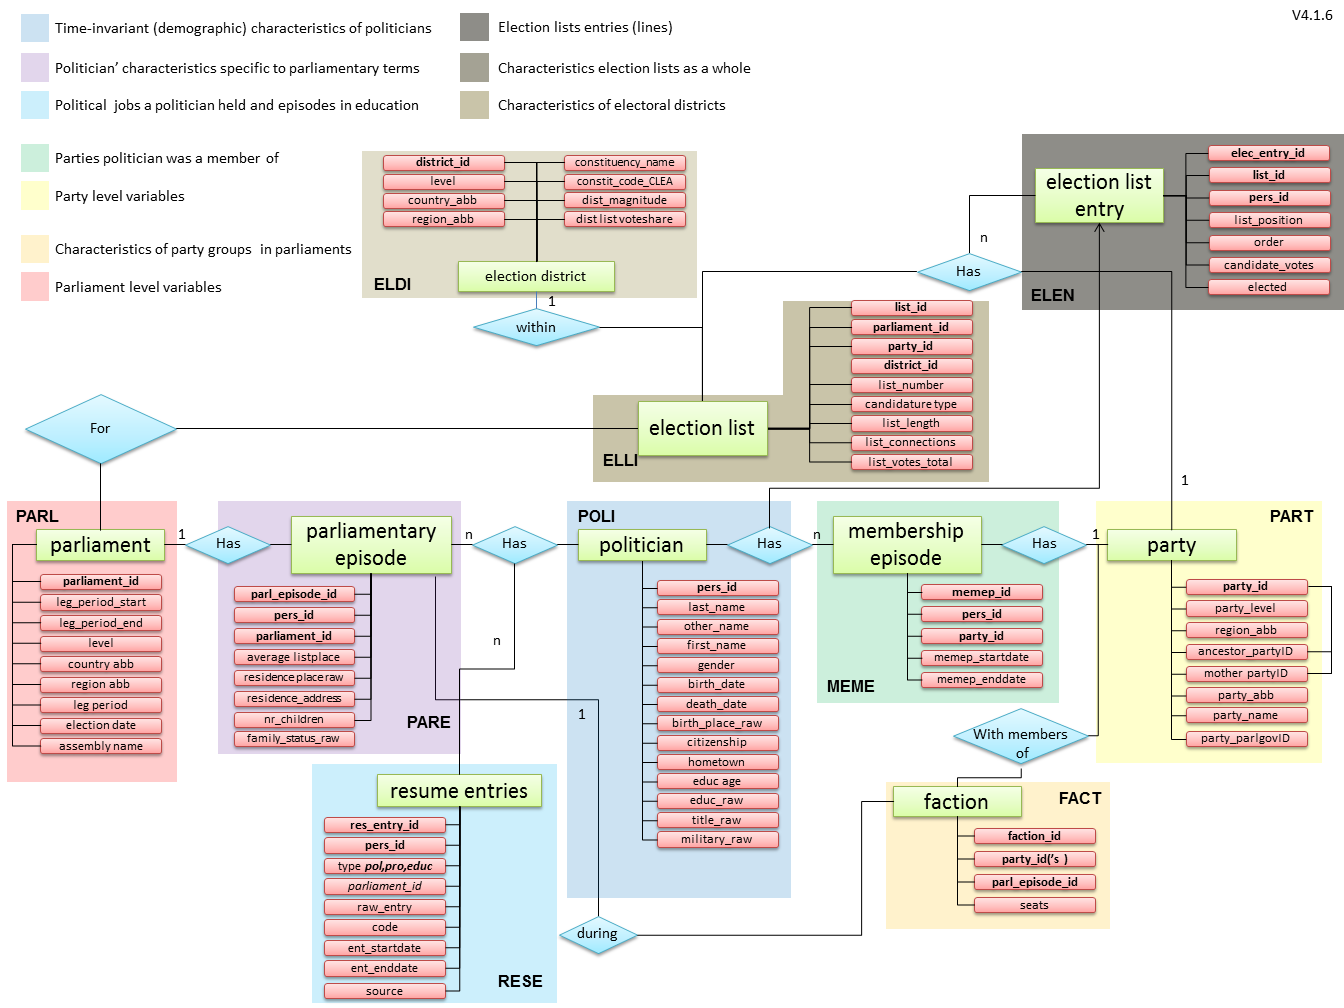
\includegraphics[width=0.95\linewidth, ]{ERdiagram.png}\label{ERdiagram}
\caption{Entity Relationship Diagram of the data}
    \label{ERdiagram}
\end{center}
\end{sidewaysfigure}

\subsection{Data Sources}
Data was collected by a combination of different \textbf{sources}. A main source for the \gls{ch} and DE parliamentary career data are yearbooks. A main source in the Netherlands was the website of the Dutch parliamentary documentation centre. Other data stem from different statistical offices or are based on newspaper articles or personal websites.\par

\subsection{Sample}
Data can be regarded a \textbf{complete (population) sample of national parliamentarians since 1946 of all three countries (\gls{ch},\gls{de}\footnote{Up until 1990 only data on West-Germany is included. For obvious reasons.},\gls{nl})} (wave one data collection).Both parliamentarians in the lower-house (i.e. Bundestag, Nationalrat, Tweede Kamer) and the upper-house (i.e. Staenderat, Eerste Kamer) are included. Future waves will likely include candidates for national elections in Germany and Switzerland (and maybe the Netherlands) since 1946, and of regional parliamentarians of all three countries (wave two). The data will likely also include data on the candidates for elections to regional parliaments (e.g. German Bundeslaender or Swiss Cantons).

\section{How to Read this Codebook}

\subsection{Labels, Abbreviations, Etc.} 
\begin{itemize}
    \item Brackets (`[' and `]') in variable names signify variable names. [country]\_ for example means that there will be as many of this variable (set) in the data-frame as their are countries in the data.
    \item `\gls{dnc}' means: Do Not Collect, these are specifications that are kept in codebook for reference purposes who values we do not intend to collect (to this level of detail).
    \item if a variable name contains an (by underscores) indexed element on the lists which is not used `NA' will be used a filler.
\end{itemize}


\subsection{Collection Effort Per Variable}
Not all variables are collected with the same effort. Our effort to collect different variables varies from the highest level (`Collect and follow-up until \gls{comp}lete') to the lowest level (`Collect When Easy'). These are the matching abbreviations:
\begin{itemize}
    \item \gls{comp} - Collect and follow-up until complete
    \item \gls{cwa} - Collect when available
    \item \gls{cwe} - Collect when easy
\end{itemize}

\newpage

\section{Politician Level Data Frame (\gls{POLI})}\label{POLI} 
Politician level variables are all static variables on the level of individual politicians. Example data can be found \href{http://parliamentarycareersincomparison.org/wp-content/uploads/2017/03/DF.xlsx}{\underline{here} (.xlsx download).}

% set columns with


    \begin{longtable}[H!]
        {|m{.18\textwidth}|
          m{.08\textwidth}|
          m{.22\textwidth}| 
          m{.30\textwidth}|
          m{.07\textwidth}|} 
 

\caption{Summary of Politician Level Variables (\gls{POLI})}
\label{POLItab}
% first line 
 \\\hline NAME & TYPE & VALUES/EXAMPLE\footnote{See text below table for more detailed variable specifications} & SHORT DESCRIPTION & EFFORT \\ \hline
\endfirsthead

\caption[]{Summary of Politician Level Data-frame (Continued)}
\\\hline NAME & TYPE & VALUES/EXAMPLE\footnote{See text below table for more detailed variable specifications} & SHORT DESCRIPTION & EFFORT \\ \hline
\endhead
 

% Variable 1 (example) /start copy paste here for new variables
    % first column
         \texttt{pers\_id}\footnote{To ensure compatibility of data-sets and make usage and merging of our data set easier we will add several id variables. The first one (\texttt{pers\_id}) will be constructed by us, consists of the country, last name, first name, and birth year, and is unique to parliamentarians across countries and levels. This ``naturally occuring'' or ``information-based'' ID format allows consistent IDS to be constructed across a variety of sources while minimizing the need to look-up IDS in the already collected data.} &
    % second column
        PriID & 
    % third column    
    
        \makecell*
        {
           % line 0
           [country]\\
           \_[first\_last\_name]\\
           \_[first\_first\_name]\\
           \_[year\_of\_birth]\\
           \\
            % line 1
                CH\_Abate\\ 
            % line 2
                \_Fabio\_1966\\
            % line 3
                \\
            % line 4
               DE\_Mueller\\     
            % line 5
               \_Johann\_1956dec \\
            % line 6
                \\
            % line 7
               NL\_Mark\\     
            % line 8
               \_Rutte\_1956dec-1
        } &
        
    % fourth 
      \textbf{parliamentarians individual identification code:} a combination of \texttt{country\_abb}, the \texttt{last\_name}, the``first\_name'' and the \texttt{birth\_date} &
    % Last
    \gls{comp}
        \\ \hline
% /end copy paste here for new variables
    
% Variable 3 
    % first column
         \texttt{id\_[country]\_parl} \footnote{We will add all important id variables (often numbers) that are used by important data sets and/or by the source data set. These additional id variables are mostly unique to a country and/or level and are named by the following principle: first ``id”, then a country abbreviation (see variable ``country\_abb”) and then a name or names that indicate the usage or source, all added by underscores.} & 
     % second column
        ID & 
    % third column
        \makecell*
        {
        2739 = Gobbi, Norman
        } &
    % last column
    \textbf{paliamentsdienst \gls{ch} identification number:} identification number, as used by the \gls{ch} Paliamentsdienst &
        % Really Last
      \gls{cwa} 
       \\ \hline
       
% Variable 5
    % first column
        \texttt{last\_name} & 
     % second column
        String & 
    % third column
        \makecell*
        {Mueller\\
        deCourten\\
        Mutlu-Blum
        } &
    % last column
    \textbf{parliamentarian' last name:} contains the last name. With `von' e.t.c. connected (space removed), double last names hyphenated and special characters replaced. &
    % Really Last
    \gls{comp} 
      \\ \hline
      
% Variable 8
    % first column
        \texttt{first\_name} 
        & 
     % second column
        String & 
    % third column
        \makecell*
        { ``Jules-Henri''\\
                ``Elisabeth''\\
                ``Johann-Ulrich-Werner''\\
                ``Heinrich-E.''
        } &
    % last column
    \textbf{parliamentarian' first name:} contains the first name. With double first names hyphenated and special characters replaced.&    
    % Really Last
    \gls{comp}
       \\ \hline
       
% Variable 6
    % first column
        \texttt{other\_name}
        & 
     % second column
        String & 
    % third column
        \makecell*
        {Hans\\
        Muller
        } &
    % last column
    \textbf{parliamentarian' alternative name or alias:} contains an (array of) - first or last - name(s) or alias(ses). For matching purposes. &

    % Really Last
      \gls{cwa} 
       \\ \hline
       
% Variable 9
    % first column
        \texttt{gender} 
        & 
     % second column
        Factor & 
    % third column
        \makecell*
        {m = male\\
        f = female\\
        nb = non-binary \\
        tm = trans male \\
        tf = trans female
        } &
    % last column
    \textbf{parliamentarian' gender}&    
    % Really Last
    \gls{comp} 
      \\ \hline
       
% Variable 10
    % first column
       \texttt{birth\_date} 
       & 
    % second column
        Date & 
    % third column
        \makecell*
        {16apr1897\\
        29may1930
        } &
    % last column
    \textbf{parliamentarian' birth date}&    
    % Really Last
      \gls{comp} 
       \\ \hline
       
% Variable 11
    % first column
        \texttt{death\_date} 
        & 
    % second column
        Date & 
    % third column
        \makecell*
        {16apr1897\\
        29may1930
        } &
    % last column
    \textbf{date of death of a parliamentarian} empty if still alive and NA when unknown&    
    % Really Last
      \gls{cwa} 
      \\ \hline
       
% Variable 12
    % first column
        \texttt{birth\_place\_raw} 
        & 
     % second column
        String
        & 
    % third column
        \makecell*
        {``Berlin''\\
                ``Zuerich''\\
                ``Baden-Wuerttemberg''
        } &
    % last column
    \textbf{place of birth:} place of birth of the parliamentarian &    
    % Really Last
      \gls{cwa} 
       \\ \hline
       
% Variable 15
    % first column
        \texttt{citizenship} 
        & 
    % second column
        String & 
    % third column
        \makecell*
        {\gls{de} \\ 
         DE; SK \\ 
         \gls{ch}
        } &
    % last column
    \textbf{parliamentarians citizenship(s):} Array of - citizenship(s) as country abbreviation(s) &    
    % Really Last
      \gls{cwa} 
       \\ \hline
       
% Variable 16
    % first column
        \texttt{citizenship\_canton} 
        & 
     % second column
        String & 
    % third column
        \makecell*
        {``\gls{zh}''
        } &
    % last column
    \textbf{Swiss canton of citizenship:} Switzerland-specific variable. Array of - citizenship(s) as canton abbreviation(s). Contains all citizensships over the entire lifetime. &    
    % Really Last
      \gls{cwa} 
      \\ \hline
      
% Variable 16a
    % first column
        \texttt{hometown\_raw} 
        & 
     % second column
        String 
        & 
    % third column
        \makecell*
        {``Fehraltorf''
        } &
    % last column
    \textbf{Hometown of a person:} Switzerland-specific string variable. Name (and description) of place/city/municipality that is the candidates/parliamentarians home town.&    
    % Really Last
      \gls{cwa} 
      \\ \hline
 
% Variable 21
    % first column
        \texttt{educ\_age} 
        &
    % second column
        Integer 
        & 
    % third column
       \makecell*{0 - 100} &
    % last column
    \textbf{age at completion of education:} ratio variable indicating how old a politician was when he/she finished her last degree&    
    % Really Last
      \gls{cwa}
    
      \\ \hline
    
% Variable 21.5
    % first column
        \texttt{educ\_raw} 
        &
    % second column
        String & 
    % third column
       \makecell*{School `The Bear' 1932} &
    % last column
    \textbf{education:} raw text string field with all available educational information &     
    % Really Last
    \gls{comp}

      \\ \hline
      
      % Variable 21.7
    % first column
        \texttt{title\_raw} 
        &
    % second column
        String & 
    % third column
       \makecell*{Prof. Dr.} &
    % last column
    \textbf{academic title:} Academic title(s), if any.\footnote{In case it is known that the MP has no academic title, this variable is set to "none".}  &     
    % Really Last
    \gls{comp}

      \\ \hline

% Variable 22
    % first column
        \texttt{military\_raw} 
        &
    % second column
        String & 
    % third column
         \makecell*{
         Major \\
         Appointé \\
        } &
    % last column
    \textbf{military rank:} raw string information about the military career&    
    % Really Last
      \gls{cwa} \\  
      \hline
      % Variable 23
    % first column
        \texttt{twitter\_screen\_name} 
        &
    % second column
        String & 
    % third column
         \makecell*{
         Petra\_Sitte\_MdB \\
         KathyR111 \\
        } &
    % last column
    \textbf{twitter screen name:} raw string information about the twitter screen name of parliamentarians, this screen name can be changed&    
    % Really Last
      \gls{cwa} \\  
      \hline

      % Variable 24
    % first column
        \texttt{twitter\_id} 
        &
    % second column
        Integer & 
    % third column
         \makecell*{
         17535941 \\
         2179010672
 \\
        } &
    % last column
    \textbf{twitter id :} this id refers to the specific account and can not be changed&    
    % Really Last
      \gls{cwa} \\  
      \hline

% Variable 25
    % first column
        \texttt{facebook\_username} 
        &
    % second column
        String & 
    % third column
         \makecell*{
         john.doe \\
         janedoe123 \\
         100009711991629
        } &
    % last column
       \textbf{facebook username :} this is a unique identifier for users on Facebook, which is sometimes numerical has sometimes been changed by the user. For latest version, query again from wikidata when possible.&    
    % Really Last
      \gls{cwa} \\  
    \hline

\end{longtable} 

%%%%%%%%%%%%%%%%%%%%%%%%%%%%%%%%%%%%%%%%%%%%%%%%%%%%%%%%%%%%%

\paragraph{pers\_id}
    \textbf{parliamentarians individual primary identification code:} Identification code, individual to each parliamentarian across levels. The code consists of the country abbreviation (as specified in variable  \texttt{country\_abb}), the last name (as specified in variable \texttt{last\_name}). The first name (as specified in \texttt{first\_name}) and the year of birth (as specified by the last four digits of variable \texttt{birth\_date}) connected by underscores. In case this id is not unique to one person, the month of birth (as specified in the middle of the \texttt{birth\_date} variable string) is appended by underscore. If the month of birth is not known or does still not uniquely identify the person, an additional index -'x' is appended (additionally to the month of birth) by hyphen. If a birth-year is unknown this the part of this identification string will be written as `9999'. In case the first name or the last name are unknown, this the part of this identification string will be written as `XXX'. As soon as the information becomes know this placeholder is replaced with the actual value (name or year). Alternative IDs and how they correspond to the main ID can be found in the appendix.

\paragraph{last\_name \& first\_name}\\
     \textbf{For the cleaning of names} the following rules apply: 

     \begin{itemize}
    \item Names always start with a capital letter
    \item an umlaut (ö,ä,ü) is written as ``oe”, ``ae”, ``ue”
    \item a ``ß” will be written as ``ss”
    \item all accents or similar (é, ã, ê, š, ğ, ç, ÿ) are left out, instead just the basic letter is written (e, a, e, s, g, c, y).
    \item if names contains prepositions like  `Von ` or ` Van der' then the space between these prepositions (name-particle) and the actual lastname are removed and capitals are replaced. So, `Von Liebig' is spelled as `vonLiebig' and `Van Der Maden' is spelled as `vanderMaden'.
    \item if the names contain multiple parts (e.g. first\_name Jean Luc) then the spaced are replaced with hypens (e.g. Jean-Luc)
    \item Additional non-name particles such as junior are included after underscores (Carl\_jun).
    \end{itemize}

\paragraph{last\_name}
    \textbf{parliamentarians last name:} The last name(s) of the parliamentarian, following the cleanup rules specified above.
        
\paragraph{first\_name}
    \textbf{parliamentarians first name:} The first name(s) of the parliamentarian, following the cleanup rules specified above.  
       
\paragraph{other\_name}
    \textbf{parliamentarians alternative names or alias:} Contains an (array of) - first or last - name(s) or alias(ses) in case there is or was another first or last name used than mentioned in ``first\_name'' or \texttt{last\_name}. This might be due to name change, a maiden name, or a commonly used shortage or alias.

\paragraph{gender} 
    \textbf{parliamentarians gender:} Gives the gender of the parliamentarian in string format. With 'm' signifying male and 'f' signifying female.

\paragraph{birth\_date}
 \textbf{parliamentarians birth date:} Mentions the date of birth of a parliamentarian consisting of the two-digit day, the month (first three letters, small, of the English name of the month) and the four-digit year of birth. If only the month is known the the days are dropped and of only the years are know the day and month letters are dropped.

\paragraph{death\_date}
    \textbf{parliamentarians death date:} Mentions the date of death of a parliamentarian consisting of the two-digit day, the month (first three letters, small, of the English name of the month) and the four-digit year of death. Is empty if still alive at the moment of data-collection and NA when unknown.
    \par\textit{Effort: collect for those who died `in office' and limit to MPs.}

\paragraph{citizenship}
    \textbf{parliamentarians citizenship(s):} Mentions the parliamentarians - array of - citizenship(s) by mentioning the abbreviation of country(s) he/she is citizen of. The used abbreviations follow the ISO ``ALPHA-2'' code. (See: \url{http://www.nationsonline.org/oneworld/country\_code\_list.htm})

\paragraph{Citizenship\_Canton}
    \textbf{Swiss canton of citizenship:} This variable is Switzerland-specific and contains the abbreviation of the canton(s) in which a parliamentarian holds municipal citizenship(s). If several municipal citizenships exist, the abbreviations are separated by semicolon. Municipal citizenship is inherited from the parents or obtained by way of naturalisation. The same abbreviation is used as in variable ``region\_abb”

\paragraph{hometown\_raw}
\textbf{hometown of a person:} Switzerland-specific string variable. Name (and description) of place/city/municipality that is the candidates/parliamentarians home town.

\paragraph{educ\_age}
    Politician its age when finished highest degree (with Diploma).
    
\paragraph{educ\_raw}
    Is a text (string) field containing all available information (in the original fora and language) on the education of a person.

\paragraph{military\_string }
    String variable with all information available on the military rank of the politician (in the original form and language).
    
    \paragraph{twitter\_screen\_name\_string }
    raw string information about the twitter screen name of parliamentarians, this screen name can be changed.
    
    \paragraph{twitter\_id\_integer }
     this id refers to the specific account and can not be changeds.

\section{Parliamentary Episode Data Frame (\gls{PARE})}\label{PARE}
    The parliamentary episode data-frame contains information that varies across parliamentary episodes. This data-frame connects the parliament (PARL) data-frame with the politician (POLI) data-frame. It contains the crucial information of what politician was in what parliament and stores additional information that is typically available with this resolution. The data-frame does not only contain elected politicians and the parliament they were member of, but also candidates. Candidates are associated to the parliament they ran for. Several time-varying variables are collected for which we know they vary across episodes but on which we do not have more detailed time-stamped information. For example, the number of children. Naturally, this would also be the data-level where a lot of parliamentary behavior variables end up in.
    
        \begin{longtable}[H!]
        {|m{.20\textwidth}|
          m{.08\textwidth}|
          m{.22\textwidth}| 
          m{.30\textwidth}|
          m{.07\textwidth}|} 

    \caption{Summary of the Parliamentary Episode Level Variables (\gls{PARE})}\label{PAREtab}\\\hline
    
% first line 
 NAME & TYPE & VALUES/EXAMPLE\footnote{See text below table for more detailed variable specifications} & SHORT DESCRIPTION & EFFORT \\ \hline
 
            % Variable 01
                % first column
                    \texttt{parl\_episode\_id} & 
                 % second column
                    PriID & 
                % third column
                       \makecell*
                {
                    % line 1
                        CH\_Abate\\ 
                    % line 2
                        \_Fabio\_1966\\
                    % line 3
                        \_\_CH\_NT-NR\_1946\\
                } &
                % last column
                \textbf{parliamentary episode ID} combination of pers\_id and  parliament\_id &
                % Really Last
                  \gls{comp} \\ \hline
                   

        % Variable 1 (example) /start copy paste here for new variables
            % first column
                 \texttt{pers\_id} &
            % second column
                String & 
            % third column    
            
                \makecell*
                {
                    % line 1
                        CH\_Abate\\ 
                    % line 2
                        \_Fabio\_1966\\
                } &
            % fourth 
              See above. A politician is considered a part of a specific parliament as soon as he/she has spend at least one day in the parliament. &
            % Last
            \gls{comp} \\ \hline
                   
                   
                      % Variable 2
              % first column
                     \texttt{parliament\_id} &
                % second column
                    String & 
                % third column 
                \makecell*
                    {
                        % line 0
                            [country]\_[level]\\
                            -[abbr]\_firstyear\\
                            \\
                        % line 1
                            NL\_NT\_1946\\
                        % line 2
                    } &
                % fourth 
                \textbf {parliament identifier:} See the specification below. &
                % Last
                \gls{comp} \\ \hline

            % Variable 41
                % first column
                    \texttt{member\_ofthisparliament\_atsomepoint} & 
                 % second column
                    String & 
                % third column
                    \makecell*
                    {"yes"\\
                            "no"\\
                    } &
                % last column
                \textbf{member of this parliament at some point:} dummy indicating, whether someone wa in the current parliament or not&    
                % Really Last
                  \gls{COMP} 
                   \\ \hline
                   
            % Variable 13
                % first column
                    \texttt{residence\_place\_raw} & 
                 % second column
                    String & 
                % third column
                    \makecell*
                    {“Mecklenburg”\\
                            ``Zuerich”\\
                            ``Essen''
                    } &
                % last column
                \textbf{place of residence raw:} all available information on the place a parliamentarian lives in&    
                % Really Last
                  \gls{cwa} 
                   \\ \hline


            % Variable 14
                % first column
                    \texttt{residence\_address} & 
                % second column
                    String & 
                % third column
                    \makecell*
                    {``Bismarkstrasse 57,  \\ 10627 Berlin''
                    } &
                % last column
                \textbf{residence\_address:} complete residential address of the parliamentarian, only full address otherwise ``residence\_place\_raw” is used&    
                % Really Last
                  \gls{cwe} \\ \hline

            % Variable 15
                % first column
                    \texttt{residence\_address\_longi} & 
                % second column
                    String & 
                % third column
                    \makecell*
                    {``Bismarkstrasse 57,  \\ 10627 Berlin''
                    } &
                % last column
                    longitude of the residence address &    
                % Really Last
                  \gls{cwe} \\ \hline


            % Variable 15b
                % first column
                    \texttt{residence\_address\_lati} & 
                % second column
                    String & 
                % third column
                    \makecell*
                    {``Bismarkstrasse 57,  \\ 10627 Berlin''
                    } &
                % last column
                latitude of the residence address &    
                % Really Last
                  \gls{cwe} \\ \hline



        % Variable 16b
            % first column
                \texttt{family\_status\_raw} & 
            % second column
                String & 
            % thirth column
                \makecell*
                {'Widowed'\\
                } &
            % last column
            \textbf{any (other) family information}, in a raw-text format &    
            % Really Last
              \gls{cwa} \\ \hline
       
        % Variable 17
            % first column
               \texttt{married} & 
            % second column
                Binary & 
            % thirth column
                \makecell*
                {1 = 'married'\\
                0 = 'not married'\\
                } &
            % last column
            \textbf{parliamentarian its marital status:}, including registered partnerships&    
            % Really Last
              \gls{cwa} \\ \hline
       
        % Variable 18
            % first column
               \texttt{nr\_children} & 
            % second column
                Integer & 
            % third column
                \makecell*
                {0:15 
                } &
            % last column
            \textbf{number of children} &    
            % Really Last
              \gls{cwa} \\ \hline
               
\end{longtable} 

\paragraph{parl\_episode\_id}
    \textbf{unique identifier of the parliament}. Combination of the ...

\paragraph{birth\_place\_raw}
    \textbf{place of birth:} Mentions the place of birth of the parliamentarian. The ``place” that is mentioned may be very specific (e.g. street, city) to very broad (e.g. district or state). Which one is mentioned depends on the information available. In case more than one information/level of detail is available, the information is appended to the existing information by a semi-colon. As for the spelling of the names, the same rules apply as for the last\_name\_full (see ``last\_name\_full''). In case the place has different names in different languages and these are available, the name in the local language is chosen.

\paragraph{residence\_place\_raw}
    \textbf{place of residence:} Mentions the place a parliamentarian lives in. The ``place” that is mentioned may be very specific (e.g. city) to very broad (e.g. district or state). Which one is mentioned depends on the information available. In case more than one information/level of detail is available, the information is appended to the existing information by semicolon. In case we have the full address of residence (i.e. street name, house number and city with postcode), the information is recorded in variable ``residence\_address”. As for the spelling of the place names, the same rules apply as for the last\_name\_full (see ``last\_name\_full''). In case different place names exist in different languages and are available, the name in the local language is chosen. (see variable ``birth\_place”)

\paragraph{residence\_address}
    \textbf{residence\_address:} Complete residential address of the parliamentarian. Only full addresses are mentioned (otherwise use the variable ``residence\_place\_raw”). The house number is separated from the street name by a blanc space, the city name and code are separated from the street name and house number by a comma. As for the spelling of the street and city names, the same rules apply as for the last\_name\_full (see ``last\_name\_full''). In case different names exist in different languages and are available, the name in the local language is chosen (see variable ``birth\_place”).
    
\paragraph{married}
    \textbf{parliamentarian was married at entry:} Dummy variable capturing whether a parliamentarian was married (or in a registered partnership). Time-varying. If the status is not known, then the status during the last parliamentary term is used. 
    
    
\paragraph{family\_status\_raw}
    \textbf{family status raw:} the raw - in own words - description of one' relationship status. If the status is known, but not when then the last parliamentary term is used. 
    
\paragraph{nr\_children}
    \textbf{number of children:} Numeric variable that captures the number of children a parliamentarian has. Time-varying.  If the status is not known, then the status during last parliamentary term is used. 
    In the case of conjoined twins, the number of brains are counted. 


%%%%%%%%%%%%%%%%%%%%%%%%%%%
%RESE SECTION
%%%%%%%%%%%%%%%%%%%%%%%%%%%
\section{Resume Entries Data Frame (\gls{RESE})}\label{RESE}

    \paragraph{What are resume entries?} In a nutshell, resume entries refer to the multitude of experiences, activities, and positions that individuals have held throughout their careers. It answers the question who held what political job when. This data-frame contains a long list of all functions (political- and non-political jobs and side-functions) that MPs held throughout their (political) career. Functions are defined as \textit{all position politicians can hold}. This entails paid and unpaid functions as well as full-time and part-time ones. It can be as big as being a prime-minister and as a small as a short voluntary activity for a local sport-club. Everything that entails an activity that a politician considers worth reporting on their resume is included. Each politician occurs multiple times in this data. A politician that held a total of 20 different (political) functions throughout her career will occupy 20 lines in this data-frame. A complete resume entry contains reference to the role somebody played in an organization, the name of the organization, where in the organization this individual played this role and a start and end-date. 
    
    A typical resume entry as used in biographies and CVs contains a description of the activity as well as a start and an end date.
    \paragraph{} The RESE therefore collects all resume entry variables and variables directly based on or related to these entries. 

% set columns with

    \begin{longtable}[H!]
        {|m{.18\textwidth}|
          m{.06\textwidth}|
          m{.22\textwidth}| 
          m{.30\textwidth}|
          m{.08\textwidth}|} 
\caption{Summary of the Resume Entry Variables (\gls{RESE})}
\label{TableWithSummaryOfRESE}
\\\hline
% first line 
 NAME & TYPE & VALUES/EXAMPLE\footnote{See text below table for more detailed variable specifications} & SHORT DESCRIPTION & EFFORT \\ \hline


% Variable 2
    % first column
         \texttt{res\_entry\_id} &
    % second column
        String & 
    % third column       
         \makecell*
        {
           % line 0
           [country\_abb]\\
           \_[first\_last\_name]\\
           \_[first\_first\_name]\\
           \_[year\_of\_birth]\\
           \_\_[number]\\
           \\
           % line 1
                CH\_Abate\\ 
            % line 2
                \_Fabio\_1966\_\_01\\
            % line 3
                \\
            % line 4
               DE\_Mueller\\     
            % line 5
               \_Johann\_1956\_dec\_\_06
        } &
    % fourth 
      \textbf{parliamentarians' resume entry code:} a combination of ``pers\_id'' and an index for the number of the entry that counts from 01 to .. &
    % Last
    \gls{comp} \\ \hline

% Variable 1 (example) /start copy paste here for new variables
    % first column
         \texttt{pers\_id} &
    % second column
        String & 
    % third column    
    
        \makecell*
        {
            % line 1
                CH\_Abate\\ 
            % line 2
                \_Fabio\_1966\\
            % line 3
                \\
            % line 4
               DE\_Mueller\\     
            % line 5
               \_Johann\_1956\_dec
        } &
    % fourth 
      \textbf{parliamentarians' individual identification code:} a combination of \texttt{country\_abb}, the \texttt{last\_name}, the \texttt{first\_name} and the \texttt{birth\_date} &
    % Last
    \gls{comp} \\ \hline
    
    
    
% Variable 3
    % first column
         \texttt{res\_entry\_type} &
    % second column
        Integer & 
    % third column    
    
        \makecell*
        {
            % line 1
            \\
            % line 2
               pol = Political\\  
            % line 3
               prof = Professional\\ 
            % line 5
               educ = Educational\\ 
             % line 6
               iden = Occupational Identity\\ 
               \\
             % line 7
               oth = Other\\ 
               \\
        } &
    % fourth 
      \textbf{parliamentarians' resume entry type:} Categorical variable that defines the type of resume entry: Entries can refer to political (1), professional (2), or educational (3) sequences. &
    % Last
    \gls{comp} \\ \hline

% Variable 4
    % first column
         \texttt{res\_entry\_start} &
    % second column
        Date & 
    % third column    
        \makecell*
        {29apr1976\\
        aug1953\\
        2012\\
        } &
    % fourth 
      \textbf{resume entry start date:} Variable that captures when a specific resume entry started. &
    % Last
    \gls{comp} \\ \hline

% Variable 5
    % first column
         \texttt{res\_entry\_end} &
    % second column
        Date & 
    % third column    
        \makecell*
        {29apr1976\\
        aug1953\\
        2012\\
        } &
    % fourth 
      \textbf{resume entry start date:} Variable that captures when a specific resume entry ended. &
    % Last
    \gls{comp} \\ \hline
 
% Variable 5.5
    % first column
         \texttt{res\_entry\_at} &
    % second column
        Date & 
    % third column    
        \makecell*
        {29apr1976;aug1953\\
        2012\\
        } &
    % fourth 
      \textbf{array of at date} (array of) dates indicating that this postion was held at this point in time. &
    % Last
    \gls{comp} \\ \hline 


% Variable 6
    % first column
         \texttt{res\_entry\_raw} &
    % second column
        String & 
    % third column 
    \makecell*
        {
            % line 1
                Conseiller communal de\\
                1970 à 1978.\\
        } &
    % fourth 
    \textbf {raw entry:} The resume entry as is taken from the source. &
    % Last
    \gls{comp} \\ \hline  
    
% Variable 6
    % first column
         \texttt{res\_entry\_source} &
    % second column
        String & 
    % third column 
    \makecell*
        {
            % line 1at
                Parlement.CH \\
                CH Yearbooks \\
        } &
    % fourth 
    \textbf {raw entry:} The resume entry as is taken from the source. See appendix XX for an overview of used RESE sources.  &
    % Last
    \gls{comp} \\ \hline  

% Variable 6
    % first column
         \texttt{res\_entry\_index} &
    % second column
         Integer & 
    % third column 
    \makecell*
        {
            % line 1
                01 \\
                02\\
        } &
    % fourth 
    \textbf {raw entry:} The position of the entry in the source. e.g. 1 means first mentioned. 2 means second etc  &
    % Last
    \gls{comp} \\ \hline  

% Variable 8
    % first column
         \texttt{political\_function} &
    % second column
         String & 
    % third column 
    \begin{tabular}{@{}c@{}}
    
                \-[PrimaryCode1]\_ \\
                \-[PrimaryCode2]- \\
                \-[SecondaryCode2]\_ \\
                \-[PrimaryCode3]- \\
                \-[SecondaryCode3]\_ \\
                \-[PrimaryCode3]\_ \\
                \-[PrimaryCode4]\_ \\
                \-[PrimaryCode5]\_ \\
                \\
                RE\_PA-MA\_T1\_300\_09 \\
                NT\_LE\_T2-CO\_1500\_03 \\
                MU\_EX\_T3\_900\_03\\
                
    \end{tabular} &
    % fourth 
    \textbf {political function:} Code assigned to the raw entry depending if it is of type ``political''. &
    % Last
    \gls{comp} \\ \hline

% Variable 8.1
    % first column
         \texttt{pf\_geolevel} &
    % second column
         String & 
    % third column
    \makecell*
        {
                \-[PrimaryCode1]\\
                \\
                RE\\
                NT\\
                MU\\
        } &
    % fourth 
    \textbf {geographical level:} Code assigned to level in the multi-level political system (see \ref{level1}) &
    % Last
    \gls{comp} \\ \hline 

% Variable 8.2
    % first column
         \texttt{pf\_instdomain} &
    % second column
         String & 
    % third column 
    \makecell*
        {
                \-[PrimaryCode2]-\\
                \-[SecondaryCode2]\\
                \-[PrimaryCode2]\\
                \\
                PA-MA\\
                LE\\
                EX\\
        } &
    % fourth 
    \textbf {institutional domain} Code assigned to the raw entry according to institutional domain, e.g. party or legislative e.t.c. (see \ref{level2}) &
    % Last
    \gls{comp} \\ \hline  

% Variable 8.3
    % first column
         \texttt{pf\_orglevel} &
    % second column
         String & 
    % third column 
    \makecell*
        {
                \-[PrimaryCode3]-\\
                \-[SecondaryCode3]\\
                \-[PrimaryCode3]\\
                \\
                T1\\
                T2-CO\\
                T3\\
        } &
    % fourth 
    \textbf {tier in the organizational hierarchy:} Code assigned to the raw entry according to general location of the position in the organizational hierarchy. (see \ref{level3}) &
    % Last
    \gls{comp} \\ \hline  

% Variable 8.4
    % first column
         \texttt{pf\_policy\_area} &
    % second column
         String & 
    % third column 
    \makecell*
        {
                \-[PrimaryCode4]\\
                \\
                0300\\
                1500\\
                0900\\
        } &
    % fourth 
    \textbf {related policy area (CAP)} Code assigned to the raw entry according to adjusted version of the Comparative Agenda's Project policy areas (see \ref{level4}) &
    % Last
    \gls{comp} \\ \hline  

% Variable 8.5
    % first column
         \texttt{pf\_position} &
    % second column
         String & 
    % third column 
    \makecell*
        {
                \-[PrimaryCode5]\_ \\
                \\
                09 \\
                03 \\
                03\\
        } &
    % fourth 
    \textbf {Type of position} Code assigned to the raw entry according to type of position, e.g. regular member or chair e.t.c. (see \ref{level5}) &
    % Last
    \gls{comp} \\ \hline  

% Variable 9
    % first column
         \texttt{parliament\_id('s)} &
    % second column
        String & 
    % third column 
    \makecell*
        {
            % line 1
                [country\_abb]\_[level]\_[year]\\
            % line 2
                NL\_NT\_1946\\
            % line 3
                DE\_NT\_2009\\
            % line 4
                CH\_NT\_1971\\
                \\
            % line 5
                \-[country\_abb]\_[level]\\
            % line 6    
                -[reg\_abb]\_[year]\\         
            % line 7
               CH\_RE-BS\_1997\\     
            % line 8
               DE\_RE-BW\_1956\\
        } &
    % fourth 
    \textbf {parliament identifier:} Unique code for different parliaments, both across countries/levels and over time. Used if political\_function refers to a certain parliament(s). Is an array seperated by ' ; '  when there are multiple parliaments &
    % Last
    \gls{comp} &
    
        \hline   



% Variable 10
    % first column
         \texttt{prof\_field} &
    % second column
        Integer & 
    % third column 
    \makecell*
        {
            % line 1
                100:2300\\
        } &
    % fourth 
    \textbf {professional field:} Professional field codes based on the CAP / U.S. Standard Industrial Classification (cf. pf\_policy\_area of the political functions primary codes) assigned to the raw entry depending if it is of type ``professional''. &
    % Last
    \gls{DNC} &
    
        \hline



% Variable 11
    % first column
        \texttt{educ\_level\_isced2011} &
    % second column
        Integer & 
    % third column 
    \makecell*
        {
            % line 1
                1:8\\
        } &
    % fourth 
    \textbf {educational level:} ISCED level code assigned to the raw entry depending if it is of type ``eductational''. &
    % Last
    \gls{comp} &
    
        \hline

% Variable 12
    % first column
        \texttt{educ\_field\_isced2013} &
    % second column
        Integer & 
    % third column 
    \makecell*
        {
            % line 1
                00:10\\
        } &
    % fourth 
    \textbf {educational field:} ISECD field code assigned to the raw entry depending if it is of type ``eductational''. &
    % Last
    \gls{comp} &
      \hline
      
      % Variable 13
    % first column
        \texttt{occ\_identity\_raw} &
    % second column
        string & 
    % third column 
    \makecell*
        {
            % line 1
                e.g. lawyer, student,\\
                 teacher, businessman\\
        } &
    % fourth 
    \textbf {occupational identity:} mentions what individuals identify as their occupation or profession at a certain point in time, in original wording. &
    % Last
    \gls{cwa} &
      \hline
      
         % Variable 14
    % first column
        \texttt{occ\_identity\_code\_DE} &
    % second column
        integer & 
    % third column 
    \makecell*
        {
            % line 1
                 1:1000\
        } &
    % fourth 
    \textbf {occupational identity code:} variable mentions the occupational identity of an individual at a certain time as classified by the German electoral bureau or statistical office &
    % Last
    \gls{cwa} &
      \hline
\end{longtable} 


\paragraph{pers\_id:}\\
    Unique identification code for different politicians. See POLI for details on page \ref{POLI}.

\paragraph{res\_entry\_id:}\\
    Identification code for resume entries, individual to each parliamentarian and entry. The code consists of ``pers\_id'' and a number per entry. Numbers below 10 are written with an additional zero (e.g. 05) and connected to ``pers\_id'' by two underscores. The order of numbers is arbitrary but roughly corresponds to the order of appearance in the source. 

\paragraph{res\_entry\_type:}\\
    Categorisation of resume entries. This variable captures the type to which a certain entry can be attributed to. Entries can refer to either political (pol), professional (prof), educational (educ), an occupational identity\footnote{the job that an MP mentions when asked by the election council to summarize their main occupation so it can be mentioned on the election list} (iden), or other (oth) biographical episodes. Political functions (pol) are functions that are directly or indirectly aimed at creating and shaping policy.
 
\paragraph{res\_entry\_start:}\\
    This variable gives the start date of a particular resume entry. These date entries consist of the two-digit day, the month (first three letters, small, of the English name of the month) and the four-digit year of birth. In case of missing information on days or month, shortened versions of the date are used.
    
\paragraph{res\_entry\_end:}\\
    This variable gives the end date of a particular resume entry. These date entries consist of the two-digit day, the month (first three letters, small, of the English name of the month) and the four-digit year of birth. In case of missing information on days or month, shortened versions of the date are used.

\paragraph{res\_entry\_raw:}\\
    This variable gives the raw resume entry string. Generally this will be the text as it has been extracted from the original source. However, completeness is more important then sticking to the original source text. For example 'bis 21 oktober 2014' would be replaced with 'Mitglied des bundesrat von 12. Jun 2000 bus 21. oktober' if this concerns an RESE entry which reflects a position in the German Bundestag (NT\_LE\_T3\_NA\_01).
    
\paragraph{political\_function\_code, pf\_geolevel, pf\_instdomain, pf\_orglevel, pf\_policy\_area, pf\_position}\\
    
    Multi-level code that captures various facets of resume entries that are categorized as political under ``res\_entry\_type''. A thorough presentation of the entire political functions coding scheme is provided in the subsequent chapter!

\paragraph{parliament\_id:}\\
    Unique identification code for different parliaments. See PARL for details on page \ref{PARL}.  It is added whenever \texttt{``political\_function''} refers to a function connected to national and regional parliaments. Is an array separated by ' ; '  when there are multiple parliaments.

\paragraph{prof\_field:}\\
    This variable captures the professional area of resume entries that were categorised as professional under ``res\_entry\_type''.  
    Professional field codes are based on the CAP / U.S. Standard Industrial Classification. The coding scheme corresponds to the policy areas (level 4) of the political functions primary codes. An overview of the codes is provided in the subsequent subchapter.

\paragraph{isco08}\\
    This variable takes a value when the entry of concern is of res\_entry\_type `prof'. Professional jobs and 
    captures the professional area of resume entries that were categorized as professional (`prof') or occupational identity (`iden') under ``res\_entry\_type''. This functions are coded into the International Standard Classification of Occupations (ISCO). This code has four levels of detail or 'digits'. All four digits are used. See https://www.ilo.org/public/english/bureau/stat/isco/isco08/ for details. The main categories of ISCO-08 are:
    
        \begin{itemize}
    \setlength\itemsep{0em}
        \item ISCO-08 major group 1 – Managers
        \item ISCO-08 major group 2 – Professional
        \item ISCO-08 major group 3 – Technicians and associate professionals
        \item ISCO-08 major group 4 – Clerical support workers
        \item ISCO-08 major group 5 – Service and sales workers
        \item ISCO-08 major group 6 – Skilled agricultural, forestry and fishery workers
        \item ISCO-08 major group 7 – Craft and related trades workers
        \item ISCO-08 major group 8 – Plant and machine operators, and assemblers
        \item ISCO-08 major group 9 – Elementary occupations
        \item ISCO-08 major group 10 – Armed forces occupations
    \end{itemize}

\paragraph{educ\_level\_isced2011:}\\
    Ordinal variable capturing the level of education of particular resume entries. Based on the ISCED 2011 international coding standard, only first digit is coded. see \url{http://www.uis.unesco.org/Education/Documents/isced-2011-en.pdf} for the codes. \par
    \textbf{isced2011 levels}
    \begin{itemize}
    \setlength\itemsep{0em}
        \item ISCED level 0 – Early childhood education
        \item ISCED level 1 – Primary education
        \item ISCED level 2 – Lower secondary education
        \item ISCED level 3 – Upper secondary education
        \item ISCED level 4 – Post-secondary non-tertiary education
        \item ISCED level 5 – Short-cycle tertiary education
        \item ISCED level 6 – Bachelor’s or equivalent level
        \item ISCED level 7 – Master’s or equivalent level
        \item ISCED level 8 – Doctoral or equivalent level
    \end{itemize}

\paragraph{educ\_field\_isced2013:}\\ 
    The isced field classification see \url{http://www.uis.unesco.org/Education/Documents/isced-fields-of-education-training-2013.pdf} only the first digit is coded.\par

    \textbf{isced2013 fields}
    \begin{itemize}
    \setlength\itemsep{0em}
        \item ISCED Field 00 - Generic programmes and qualifications
        \item ISCED Field 01 - Education
        \item ISCED Field 02 - Arts and humanities
        \item ISCED Field 03 - Social sciences, journalism and information
        \item ISCED Field 04 - Business, administration and law
        \item ISCED Field 05 - Natural sciences, mathematics and statistics
        \item ISCED Field 06 - Information and Communication Technologies
        \item ISCED Field 07 - Engineering, manufacturing and construction
        \item ISCED Field 08 - Agriculture, forestry, fisheries and veterinary
        \item ISCED Field 09 - Health and welfare
        \item ISCED Field 10 - Services
    \end{itemize}

\subsubsection{left- and right censoring of dates}

    In some cases we know for sure that a career episode \textbf{at least} lasted until (or started') at a certain moment in time. Such 'censored' dates are indicated in our data with `[[lcen]]' and `[[rcen]]' respectively. If we for example know that a politician was in parliament at least from 19 Jan 1985 onward then we would write this as '19jan1985[[lcen]]'. If we would check on 31th of December 2018 and found out she is still there then res\_entry\_end\ will be written as `31dec2018[[rcen]]'

\newpage
\subsection{The (political) functions coding scheme}

To investigate political careers, we need to know who had what (political) job when. As such, a core part of our data concerns the resume entry (\sethlcolor{RESEcol}\hl{RESE}) data-frame. This data-frame contains a long list of all functions (political- and non-political jobs and side-functions) that the politicians in our data held throughout their (political) career. Functions are defined as \textit{all position politicians can hold}. This entails paid and unpaid functions as well as full-time and part-time ones. It can be as big as being a prime-minister and as a small as a short voluntary activity for a local sport-club. Everything that entails an activity that a politician considers worth reporting on their resume is included. Each politician occurs multiple times in this data. For example, a politician that held a total of 20 different (political) functions throughout her career will occupy 20 lines in this data-frame.

As the focus is on political career the majority of the functions in the RESE data-frame are 'political functions' (defined as ' functions that are directly or indirectly aimed at creating and shaping policy'). This definition is quite all encompassing on purpose; it for example also includes being the CEO of a largere company and part of her job is as well to shape polocy relevant for the company its profits. There are however also several none-political functions in the data. These are marked as 'prof' in the res\_entry\_type column. There are also several educational episodes (periods of their lives in which MPs where not working but following educational programs instead) in the data. These are marked as 'educ'. The classification scheme below is focused is our own new classification of political functions. Professional jobs are code into the excisting; ISCO-08 coding scheme (see above) and educational entries into the excisting ISCED field and level classifications (see above).

    \subsubsection{Principles for Classification of (political) functions}
    
     The proposed coding scheme for the classification of political functions consists of two parts. The first one is labelled \textbf{primary political function coding} while the second one can be referred to as \textbf{secondary political function coding}. 

        \begin{itemize}
            \item \textbf{Primary function coding} entails information that can be coded for all political functions. For example, we should be able to code all political functions with regard to the geographical level (pf\_geolevel, e.g. municipal / regional / national) they are located on in the multi-level hierarchy.
            \item \textbf{Secondary function coding} refers to information that is specific to subsets of the primary coding. With the primary coding scheme for instance, we are unable to distinguish whether some-one’s party function was in a youth party (YO) or the main party (MA). Secondary codings are therefore introduced whenever an even more detailed distinction is of interest for particular research questions.
        \end{itemize}
    
    \subsubsection{Primary Political Function Coding}
    \paragraph{pf\_geolevel: Position of organization in the multi-level hierarchy}\label{level1}
    
    Coding the position in the multi-level structure depends on the institutional affiliation of the political function (thus often answering the question \textit{who pays you?}). Example: Working as an ambassador to the EU will therefore be coded as national level (NT).\par
        \par\textit{Effort: collect until complete.}
    
    \begin{itemize}
        \item IN    - International level
        \item EU    - EU level
        \item NT    - National level
        \item SR    - Superregional level (regional, super) (below national, above regional level) 
        \item RE    - Regional level (NL: provinces; DE: Bundesländer; CH: Cantons)
        \item SD    - Superdistrictual level (districutal, super) (below regional, above district level)1
        \item DI    - District level (CH: Ämter, Bezirke; DE: Kreise)
        \item SM    - Supermunicipal level (municipal, super) (below district, above municipal level; CH: Kreise)1
        \item MU    - Municipal level
        \item BM    - Below-Municipal level (e.g. neighbohrhood counsel)

    \end{itemize}
    
    \paragraph{pf\_instdomain: Organisational type}\label{level2} \\
        \par\textit{Effort: collect until complete.}
      \begin{itemize}
        \item LE    - Legislative
        \item EX    - Executive
        \item JU    - Judiciary
        \item AD    - Administration (including dependent agencies)
        \item SI    - Semi-independent agencies
        \item PA    - Party
        \item IG    - Interest Group
        \item OT - Other
     \end{itemize}
    
    Notes with institutional domain coding:
    \begin{itemize}
        \item if you are a CEO of a large company and it is part of your job to influence policy you would be coded as organisational type: IG - Interest Group
        \item Semi-independent agencies are public bodies that resemble administrations in their behavior. They have goals defined by the state such as financial regulation (e.g. FINMA), drug licencing (SWISSMEDIC), or nuclear power safety (ENSI). Furthermore, they can also include state-owned research institutions (e.g. AGROSCOPE). They do not pursue financial goals. Publically owned companies (e.g. Swiss Federal Railways, Swisscom, Swiss Post) are therefore NOT semi-independent agencies but IGs.
    \end{itemize}
    
   \paragraph{pf\_orglevel: Internal structure of organisational types, up to 3 tiers}\label{level3} \\
             \par\textit{Effort: collect when available.}
      \begin{itemize}
        \item T1 Top-tier
        \item T2 Mid-tier
        \item T3 Low-tier
     \end{itemize}

    \paragraph{How to code the tiers}
    The terms \textit{top-tier, mid-tier, low-tier} would be used as overarching descriptions. For the specific combinations of pf\_geolevel and pf\_instdomain codes (e.g. B-A EU-level legislative), the name of the actual corresponding tier name would be used e.g. \textit{parliamentary presidency} instead of \textit{top-tier}.\par
    Institutions have highly differing structures that do not only vary across but even within countries. The use of three tiers is necessary to enable comparisons between institutions within and across countries. The tiers offer a meaningful simplification of institutional structure in terms of policy competences. Almost all institutions depict a similar structure: the highest and leading instance holding the broadest/deepest competences (T1), the unit right below the highest instance which holds specialised competences and reports to or is controlled by the highest instance (T2), and the rest of the organizational hierarchy which covers the remaining less powerful and less prestigious functions (T3).\par
    
    It should be noted that the tiers do not (necessarily) refer to a division of labor though. Support bodies tasked with administrative and implementing functions (e.g. secretariats affiliated with leadership or steering bodies) are coded on the same tier as their principals'. However, bodies to which policy competences are delegated are coded on a separate level. \par
    \newpage
    The table below serves to assist with the classification process. We can see here that almost all institutions under consideration either follow such a three tier structure or the structure can be meaningfully divided into three tiers.\par

% set columns with
    \begin{longtable}
        {|m{.08\textwidth}|
          m{.17\textwidth}|
          m{.30\textwidth}| 
          m{.31\textwidth}|} 

% first line 
 Code & Description & Categories & Examples\\ \hline

% Variable 0
    % first column
         IN-... &
    % second column
        International level &
    % third column    
    ... &

    % last column
    ... &

    % line to next row
    \hline

% Variable 1
    % first column
         EU\_LE &
    % second column
        EU-level legislative &
    % third column    
  \begin{enumerate}
    \setlength\itemsep{0em}
      \item[T1] Parliamentary presidency
      \item[T2] Committee / delegation / party group
      \item[T3] Assembly
  \end{enumerate} &

    % last column
  \begin{enumerate}
    \setlength\itemsep{0em}
      \item[T1] ``Schulz' cabinet''
      \item[T2] ``Committee on Legal Affairs”
      \item[T3] ``MEP”
  \end{enumerate} &
    % line to next row
    \hline


% Variable 2
    % first column
         EU\_EX &
    % second column
        EU-level executive &
    % third column    
  \begin{enumerate}
    \setlength\itemsep{0em}
      \item[T1] Commission presidency
      \item[T2] College of Commissioners
      \item[T3] Secretariat-General
  \end{enumerate} &

    % last column
  \begin{enumerate}
    \setlength\itemsep{0em}
      \item[T1] ``First Vice-President''
      \item[T2] ``Commissioner for Energy Union''
      \item[T3] ``Unit B3 Ethics“
  \end{enumerate} &
    % line to next row
    \hline

% Variable 3
    % first column
         EU\_JU &
    % second column
        EU-level judiciary &
    % third column
    \gls{dnc}
  \begin{enumerate}
    \setlength\itemsep{0em}
      \item[T1] European Court of Justice
      \item[T1] General Court
      \item[T1] Specialised court
  \end{enumerate} &

    % last column
  \begin{enumerate}
    \setlength\itemsep{0em}
      \item[T1] ``Third Chamber''
      \item[T1] ``Registry”
      \item[T1] ``EU Civil Service Tribunal''
  \end{enumerate} &
    % line to next row
    \hline

% Variable 4
    % first column
         EU\_AD &
    % second column
        EU-level administration &
    % third column    
  \begin{enumerate}
    \setlength\itemsep{0em}
      \item[T1] Directorate-General 
      \item[T1] Directorate / department
      \item[T1] Unit
  \end{enumerate} &

    % last column
  \begin{enumerate}
    \setlength\itemsep{0em}
      \item[T1] ``DG Communication''
      \item[T1] ``Directorate Resources“
      \item[T1] ``Energy policy coordination unit''
  \end{enumerate} &
    % line to next row
    \hline

% Variable 5
    % first column
         EU\_SI &
    % second column
        EU-level semi-independent agencies &
    % third column    
  \begin{enumerate}
    \setlength\itemsep{0em}
      \item[T1] Decision-making body
      \item[T2] Department
      \item[T3] Unit
  \end{enumerate} &

    % last column
  \begin{enumerate}
    \setlength\itemsep{0em}
      \item[T1] ``ECB’s executive board”
      \item[T2] ``Department of air and climate change”
      \item[T3] ``Nutrition unit''
  \end{enumerate} &
    % line to next row
    \hline

% Variable 6
    % first column
         EU\_PA &
    % second column
        EU-level party &
    % third column    
  \begin{enumerate}
    \setlength\itemsep{0em}
      \item[T1] Party leadership body
      \item[T2] Steering body(commission, delegation, council, `bureau', non-administrative secretariat)
  \end{enumerate} &

    % last column
  \begin{enumerate}
    \setlength\itemsep{0em}
      \item[T1] ``Presidency”
      \item[T2] ``PES Council''

  \end{enumerate} &
    % line to next row
    \hline

% Variable 7
    % first column
         EU\_IG &
    % second column
        EU-level interest group &
    % third column    
  \begin{enumerate}
    \setlength\itemsep{0em}
      \item[T1] Leadership body
      \item[T2] Steering body / department (committee, delegation, council, bureau, secretariat, office)

  \end{enumerate} &

    % last column
  \begin{enumerate}
    \setlength\itemsep{0em}
      \item[T1] ``Board”, ``presidential council'', ``Directorate-General''
      \item[T2] ``General committee”, ``department'', ``committee”, ``working groups”, ``Brussels office”
  \end{enumerate} &
    % line to next row
    \hline
    
% Variable 8
    % first column
         EU\_OT &
    % second column
        Other EU level entities &
    % third column    
    ... &

    % last column
    ... &

    % line to next row
    \hline

% Variable 9
    % first column
         NT\_LE &
    % second column
        National parliament &
    % third column    
    \begin{enumerate}
    \setlength\itemsep{0em}
      \item[T1] Parliamentary presidency
      \item[T2] Committee / delegation / party group
      \item[T3] Assembly
    \end{enumerate} &

    % last column
    \begin{enumerate}
    \setlength\itemsep{0em}
      \item[T1] ``Nationalratspräsidentin''
      \item[T2] ``Commissie voor de Rijksuitgaven''
      \item[T3] ``MP''
    \end{enumerate} &

    % line to next row
    \hline

% Variable 10
    % first column
         NT\_EX &
    % second column
        National government &
    % third column    
    \begin{enumerate}
    \setlength\itemsep{0em}
      \item[T1] Government Leadership
      \item[T2] Ministerial Level
      \item[T3] Junior Ministerial Level
    \end{enumerate} &

    % last column
    \begin{enumerate}
    \setlength\itemsep{0em}
      \item[T1] ``Bundeskanzlerin''
      \item[T2] ``Bundesminister des Innern''
      \item[T3] ``Staatssecretaris van Onderwijs''
    \end{enumerate} &

    % line to next row
    \hline

% Variable 11
    % first column
         NT\_JU &
    % second column
        National judiciary &
    % third column
    \gls{dnc}
    \begin{enumerate}
    \setlength\itemsep{0em}
      \item[T1] Highest court
      \item[T2] Court of Appeal / 2nd highest court
      \item[T3] -
    \end{enumerate} &

    % last column
    \begin{enumerate}
    \setlength\itemsep{0em}
      \item[T1] ``Raad van State“; „Hoge Raad“, ``Bundesfinanzhof“, ``Bundesgericht''
      \item[T2] ``Bundesverwaltungsgericht''
    \end{enumerate} &

    % line to next row
    \hline

% Variable 12
    % first column
         NT\_AD &
    % second column
        National administration &
    % third column    
    \begin{enumerate}
    \setlength\itemsep{0em}
      \item[T1] Department
      \item[T2] Subdepartment
      \item[T3] Unit
    \end{enumerate} &

    % last column
    \begin{enumerate}
    \setlength\itemsep{0em}
      \item[T1] ``Secretariaat-generaal“, ``Generalsekretariat'', ``Staatssekretariat''
      \item[T2] ``Bundesamt (\gls{ch})”, „Abteilung (\gls{de})“, „Directie-Generaal“
      \item[T3] „Referat“, „Stab“, „Unterabteilung“, „Amt“ „Directie“
    \end{enumerate} &

    % line to next row
    \hline
    
% Variable 13
    % first column
         NT\_SI &
    % second column
        National semi-independent agencies &
    % third column    
    \begin{enumerate}
    \setlength\itemsep{0em}
      \item[T1] Decision-making body
      \item[T2] Department
      \item[T3] Unit
    \end{enumerate} &

    % last column
    \begin{enumerate}
    \setlength\itemsep{0em}
      \item[T1] ``Bestuur'', ``Direktion (\gls{ch})”
      \item[T2] ``Directie“, ``Abteilung“
      \item[T3] ``Team (\gls{nl})”, „Referat (\gls{de})“
    \end{enumerate} &

    % line to next row
    \hline

% Variable 14
    % first column
         NT\_PA &
    % second column
        National party &
    % third column    
    \begin{enumerate}
    \setlength\itemsep{0em}
      \item[T1] Party leadership body
      \item[T2] Steering body (commission, delegation, council, bureau, secretariat)
    \end{enumerate} &

    % last column
    \begin{enumerate}
    \setlength\itemsep{0em}
      \item[T1] ``Partijbestuur“, „Parteileitung“
      \item[T2] „Partijbureau“, ``Generalsekretariat“, „Bundesgeschäftsstelle“, „Bundesparteigericht“
    \end{enumerate} &

    % line to next row
    \hline

% Variable 15
    % first column
         NT\_IG &
    % second column
        National interest group &
    % third column    
    \begin{enumerate}
    \setlength\itemsep{0em}
      \item[T1] Leadership body
      \item[T2] Steering body / department (committee, delegation, council, bureau, secretariat, 
    \end{enumerate} &

    % last column
    \begin{enumerate}
    \setlength\itemsep{0em}
      \item[T1] ``Board”, ``presidential council'', ``Directorate-General''
      \item[T2] ``General committee”, ``department'', ``committee”, ``working groups”, ``Brussels office”
    \end{enumerate} &

    % line to next row
    \hline

% Variable 16
    % first column
         NT\_OT &
    % second column
        Other national entities &
    % third column    
    ... &

    % last column
    e.g. intercantonal concordats &

    % line to next row
    \hline
    
% Variable 17
    % first column
         SR\_ &
    % second column
       Superregional level &
    % third column    
    ... &

    % last column
    CH: 11 Kreispostdirektionen (bis 1997), 3 Kreise der Bundesbahnen (bis 1998), 4 Kreise der Zollverwaltung (bis 2000), 14 Kreise der Alkoholverwaltung NL: 5 gerechtshoven (courts of appeal in five regions) &

    % line to next row
    \hline
    
    
% Variable 17
    % first column
         RE\_LE &
    % second column
        Regional parliament &
    % third column    
    \begin{enumerate}
    \setlength\itemsep{0em}
      \item[T1] Presidency of the regional parliament
      \item[T2] Committee / delegation / faction
      \item[T3] Assembly (of the regional parliament)
    \end{enumerate} &

    % last column
    \begin{enumerate}
    \setlength\itemsep{0em}
      \item[T1] ``Parlamentspraesident'', ``Kantonsratspraesident'', ``Grossratspraesidentin'', „Landtagspraesident“
      \item[T2] ``Ausschuss fuer Laendlichen Raum und Verbraucherschutz”, ``Presidium”, ``Fractievoorzittersoverleg“
      \item[T3] ``Provinciale Staten'', „Landtag“, „Kantonsrat“, „Grossrat“     
      
    \end{enumerate} &

    % line to next row
    \hline

% Variable 18
    % first column
         RE\_EX &
    % second column
        Regional government &
    % third column    
    \begin{enumerate}
    \setlength\itemsep{0em}
      \item[T1] Regional Government Leadership
      \item[T2] Regional Ministerial Level
      \item[T3] Regional Junior Ministerial Level
    \end{enumerate} &

    % last column
    \begin{enumerate}
    \setlength\itemsep{0em}
      \item[T1] ``Ministerpraesident'', ``Comissaris van de Koning”, ``Regierungspraesident'', „Staatsratspraesidentin'',
      \item[T2] ``Gedeputeerde Staten'', ``Regierungsrat'', ``Staatsrat'', „Innenminister“
      \item[T3] ...  
      
    \end{enumerate} &

    % line to next row
    \hline

% Variable 19
    % first column
         RE-JU &
    % second column
        Regional judiciary &
    % third column    
    \gls{dns}
    \begin{enumerate}
    \setlength\itemsep{0em}
      \item[T1] Highest Court
      \item[T2] Court of Appeal/ 2nd highest court
      \item[T3] -
    \end{enumerate} &

    % last column
    \begin{enumerate}
    \setlength\itemsep{0em}
      \item[T1] ``Oberlandesgericht Karlsruhe'' (highest ordinary court) ``Rechtbank”, ``Kantonsgericht''
      \item[T2] ``Amtsgericht Achern''
    \end{enumerate} &

    % line to next row
    \hline

% Variable 20
    % first column
         RE-AD &
    % second column
        Regional administration &
    % third column    
    \begin{enumerate}
    \setlength\itemsep{0em}
      \item[T1] Department
      \item[T2] Subdepartment
      \item[T3] Unit
    \end{enumerate} &

    % last column
    \begin{enumerate}
    \setlength\itemsep{0em}
      \item[T1] ``Direktion''
      \item[T2] ``Kantonsamt (\gls{ch})”, „Abteilung (\gls{de})“, „Directie-Generaal“
      \item[T3] „Referat“, „Stab“, „Unterabteilung“, „Amt“ „Directie“
    \end{enumerate} &

    % line to next row
    \hline
    
% Variable 21
    % first column
         RE-SI &
    % second column
        Regional semi-independent agencies &
    % third column    
    \begin{enumerate}
    \setlength\itemsep{0em}
      \item[T1] Decision-making body
      \item[T2] Department
      \item[T3] Unit
    \end{enumerate} &

    % last column
    \begin{enumerate}
    \setlength\itemsep{0em}
      \item[T1] ``Bestuur'', ``Direktion (\gls{ch})”
      \item[T2] ``Directie“, ``Abteilung“
      \item[T3] ``Team (\gls{nl})”, „Referat (\gls{de})“
    \end{enumerate} &

    % line to next row
    \hline

% Variable 22
    % first column
         RE-PA &
    % second column
        Regional party &
    % third column    
    \begin{enumerate}
    \setlength\itemsep{0em}
      \item[T1] Party leadership body
      \item[T2] Steering body (commission, delegation, council, bureau, secretariat)
    \end{enumerate} &

    % last column
    \begin{enumerate}
    \setlength\itemsep{0em}
      \item[T1] ``Partijbestuur“, „Landesvorstand“, „Landespraesidium“, „Kantonalparteileitung“
      \item[T2] „Partijbureau“, „Landesgeschäftsstelle“, „Landesparteigericht“, ``Parteisekretariat''
      
    \end{enumerate} &

    % line to next row
    \hline

% Variable 23
    % first column
         RE\_IG &
    % second column
        Regional interest group &
    % third column    
    \begin{enumerate}
    \setlength\itemsep{0em}
      \item[T1] Leadership body
      \item[T2] Steering body / department (committee, delegation, council, bureau, secretariat, 
    \end{enumerate} &

    % last column
    \begin{enumerate}
    \setlength\itemsep{0em}
      \item[T1] ``Board”, ``presidential council'', ``Directorate-General''
      \item[T2] ``General committee”, ``department'', ``committee”, ``working groups”, ``Bremen office”
    \end{enumerate} &

    % line to next row
    \hline

% Variable 24
    % first column
         RE\_OT &
    % second column
        Other regional entities &
    % third column    
    ... &

    % last column
    e.g. private-public partnerships with political functions &

    % line to next row
    \hline

% Variable 24
    % first column
         SD\_ &
    % second column
    Superdistrictual level &
    % third column    
    ... &

    % last column
    NL: 19 rechtbanken (separated into judicial arrondisements), waterschapen CH: Zivilkreisgerichte  &

    % line to next row
    \hline


% Variable 25
    % first column
         DI\_LE &
    % second column
        District parliament &
    % third column    
    \begin{enumerate}
    \setlength\itemsep{0em}
      \item[T1] Presidency of the district parliament
      \item[T2] Committee / delegation / faction
      \item[T3] Assembly (of the district parliament)
    \end{enumerate} &

    % last column
    \begin{enumerate}
    \setlength\itemsep{0em}
      \item[T1] ``Kreistagspraesident'', ``Landrat''
      \item[T2] ``Ausschuss fuer Migration''
      \item[T3] ``Kreistagsabgeordnete''
    \end{enumerate} &

    % line to next row
    \hline

% Variable 26
    % first column
         DI-EX &
    % second column
        District government &
    % third column    
    \begin{enumerate}
    \setlength\itemsep{0em}
      \item[T1] District government leadership
      \item[T2] District government membership
      \item[T3] District government steering body
    \end{enumerate} &

    % last column
    \begin{enumerate}
    \setlength\itemsep{0em}
      \item[T1] ``Landrat'' ``Landrat'', ``Amtsstatthalter'', ``Regierungsstatthalter“, „Bürgerworthalter“
      \item[T2] ``Kreisvorstand”
      \item[T3] ...
    \end{enumerate} &

    % line to next row
    \hline

% Variable 27
    % first column
         DI-JU &
    % second column
        District judiciary &
    % third column
    \dnc{dnc}
    \begin{enumerate}
    \setlength\itemsep{0em}
      \item[T1] District Level Court
    \end{enumerate} &

    % last column
    \begin{enumerate}
    \setlength\itemsep{0em}
      \item[T1] ``Amtsgericht Achern'', ``Kreisgericht“, „Amtsgericht“, „Bezirksgericht“, „Kantongerecht“
    \end{enumerate} &

    % line to next row
    \hline

% Variable 28
    % first column
         DI-AD &
    % second column
        District administration &
    % third column    
    \begin{enumerate}
    \setlength\itemsep{0em}
      \item[T1] Department
      \item[T2] Subdepartment
      \item[T3] Unit
    \end{enumerate} &

    % last column
    \begin{enumerate}
    \setlength\itemsep{0em}
      \item[T1] ``Kreisamt (\gls{ch})”, ``Dezernat (\gls{de})”, ``Abteilung (\gls{de})”,
      \item[T2] ``Referat'', ``Stab”
      \item[T3] ``Unterabteilung”
    \end{enumerate} &

    % line to next row
    \hline
    
% Variable 29
    % first column
         DI-SI &
    % second column
        District semi-independent agencies &
    % third column    
    \begin{enumerate}
    \setlength\itemsep{0em}
    \item[T1] Decision-making body
    \item[T2] Department
    \item[T3] Unit
    \end{enumerate} &

    % last column
   ... &

    % line to next row
    \hline

% Variable 30
    % first column
         DI-PA &
    % second column
        District level party &
    % third column    
    \begin{enumerate}
    \setlength\itemsep{0em}
      \item[T1] Party leadership body
      \item[T2] Steering body (commission, delegation, council, bureau, secretariat)
      
    \end{enumerate} &

    % last column
    \begin{enumerate}
    \setlength\itemsep{0em}
      \item[T1] ``Partijbestuur“, „Präsidium“, „Kamerkringbestuur“, ``Geschäftsleitung”, „Bezirksvorstand“, „Kreispraesidium“, „Partijbureau“, „Kreisgeschäftsstelle“,
      \item[T2] „Kamerkring“, „Kamercentrale“, „Provinciaal contact“
    \end{enumerate} &

    % line to next row
    \hline

% Variable 31
    % first column
         DI-IG &
    % second column
        District level interest group &
    % third column    
    \begin{enumerate}
    \setlength\itemsep{0em}
      \item[T1] Leadership body
      \item[T2] Steering body / department (committee, delegation, council, bureau, secretariat, 
    \end{enumerate} &

    % last column
    \begin{enumerate}
    \setlength\itemsep{0em}
      \item[T1] ``Board”, ``presidential council'', ``Directorate-General''
      \item[T2] ``General committee”, ``department'', ``committee”, ``working groups”, ``Bremen office”
    \end{enumerate} &

    % line to next row
    \hline

% Variable 32
    % first column
         DI-OT &
    % second column
        Other district level entities &
    % third column    
    ... &

    % last column
    ... e.g. private-public partnerships with political functions &

    % line to next row
    \hline

% Variable 32
    % first column
         SM- &
    % second column
        Supermunicipal level &
    % third column    
    ... &

    % last column
    CH: ``Gemeindeverband” &

    % line to next row
    \hline  

% Variable 33
    % first column
        MU-LE &
    % second column
        Municipal parliament &
    % third column    
    \begin{enumerate}
    \setlength\itemsep{0em}
      \item[T1] Presidency of the municipal parliament
      \item[T2] Committee / delegation / faction
      \item[T3] Assembly
    \end{enumerate} &

    % last column
    \begin{enumerate}
    \setlength\itemsep{0em}
      \item[T1] ``Parlamentspraesident''
      \item[T2] ``Ausschuss''
      \item[T3] „Gemeindeparlament“, ``Einwohnerrat'', ``Stadtparlament'', ``Gemeenteraad”
    \end{enumerate} &

    % line to next row
    \hline


% Variable 34
    % first column
        MU-EX &
    % second column
        Municipal government &
    % third column    
    \begin{enumerate}
    \setlength\itemsep{0em}
      \item[T1] Municipal government leadership
      \item[T2] Municipal government membership
      \item[T3] Municipal government steering body
    \end{enumerate} &

    % last column
    \begin{enumerate}
    \setlength\itemsep{0em}
      \item[T1] „Gemeindepräsident“, „Stadtverordnetenvorsteher“, „Ratsvorsitzender“, „Präsident der Bürgerschaft“, „Bürgervorsteher“, „(Ober-)Bürgermeister“, „Burgemeester“
      \item[T2] „Gemeinderat“, „Stadtrat“, „College van burgemeester en wethouders“
      \item[T3] ``Welstand”, ``SER”, ``Einbürgerungskommission''
    \end{enumerate} &

    % line to next row
    \hline


% Variable 35
    % first column
         MU-JU &
    % second column
        Municipal judiciary &
    % third column
    \gls{dnc}
    \begin{enumerate}
    \setlength\itemsep{0em}
      \item[T1] (see District Judiciary)
    \end{enumerate} &

    % last column
   ... &

    % line to next row
    \hline

% Variable 36
    % first column
         MU-AD &
    % second column
        Municipal administration &
    % third column    
    \begin{enumerate}
    \setlength\itemsep{0em}
      \item[T1] Department
      \item[T2] Subdepartment
      \item[T3] Unit
    \end{enumerate} &

    % last column
    \begin{enumerate}
    \setlength\itemsep{0em} 
      \item[T1] ``Ressorts”, ``Amt'', ``Dezernat''
      \item[T2] ``Bereich”
      \item[T3] ``Sachbereich” 
    \end{enumerate} &

    % line to next row
    \hline
    
% Variable 37
    % first column
         MU-SI &
    % second column
        Municipal semi-independent agencies &
    % third column    
    \begin{enumerate}
    \setlength\itemsep{0em} 
    \item[T1] Decision-making body
    \item[T2] Department
    \item[T3] Unit

      
    \end{enumerate} &

    % last column
  ... &

    % line to next row
    \hline

% Variable 38
    % first column
         MU-PA &
    % second column
        Municipal party &
    % third column    
    \begin{enumerate}
    \setlength\itemsep{0em}
      \item[T1] Party leadership body
      \item[T2] Steering body (commission, delegation, council, bureau, secretariat)
    \end{enumerate} &

    % last column
    \begin{enumerate}
    \setlength\itemsep{0em}
      \item[T1] ``Partijbestuur“, „Vorstand des Ortsverbandes“, ``Geschäftsleitung“, „Präsidium“, ``Geschäftsleitung“
      \item[T2] „Partijbureau“, „Parteibüro“
    \end{enumerate} &

    % line to next row
    \hline

% Variable 39
    % first column
         MU-IG &
    % second column
        Municipal interest group &
    % third column    
    \begin{enumerate}
    \setlength\itemsep{0em}
      \item[T1] Leadership body
      \item[T2] Steering body / department (committee, delegation, council, bureau, secretariat, 
    \end{enumerate} &

    % last column
    \begin{enumerate}
    \setlength\itemsep{0em}
      \item[T1] ``Board” ``presidential council'', ``Directorate-General''
      \item[T2] ``General committee”, ``department'', ``committee”, ``working groups”
    \end{enumerate} &

    % line to next row
    \hline

% Variable 40
    % first column
         MU-OT &
    % second column
        Other municipal entities &
    % third column    
    ... &

    % last column
  ... &

    % line to next row
    \hline

\caption{Political functions pf\_orglevel coding specifications} % needs to go inside longtable environment
\label{tab:myfirstlongtable}
\end{longtable} 

While this three-tier code condenses information, the more detailed information will not necessarily be lost. On the one hand, it is still part of the string variable that is used to code the tier; on the other hand specific secondary codes can be introduced. The secondary code (see 2 Secondary Coding) can be used to introduce more specificity whenever it is required. Take for example national level parliaments and say we are particularly interested in positions in national parliamentary bodies. The primary coding does not provide detailed information on that (see table \ref{nt_le_example})

\begin{table}[H]
\begin{center}
 \begin{tabular}{|c|c|c|} 
 \hline
 Code & Description & Categories \\ [0.5ex] 
 \hline\hline
 NT-LE & 
 National parliament & 
  \makecell*{
         T1 - Parliamentary presidency \\
         T2 - Committee / party group / delegation \\
         T3 - Assembly \\
        } &
 \hline
 \end{tabular}
 \captionof{table}{Example of Three-tier Coding}\label{nt_le_example}
\end{center}
\end{table}

The information on committees, delegations, and party groups is condensed into one single category (mid-tier). If the interest arises to study membership in these different bodies separately, the secondary code would capture that (See table \ref{SecC})

\begin{table}[H]
\begin{center}
 \begin{tabular}{|c|c|c|c|} 
 \hline
 Code & Description & Categories & Secondary code options for NT-LE-02 \\ [0.5ex] 
 \hline\hline
 NT-LE & 
 National parliament & 
    
    \makecell*{
         T1 - Parliamentary presidency \\
         T2 - Committee / delegation / party group \\
         T3 - Assembly \\
        } &
    
    \makecell*{
         CO: Committee \\
         FA: Faction (party group) \\
         DL: Parliamentary delegation \\
        } &
 \hline
 \end{tabular}\caption{Example of Secondary Coding}\label{SecC}
\end{center}
\end{table}

Beyond the coding of just NT-LE-02 for national parliamentary bodies, we can thus in the same step code this additional information.
% \afterpage{\clearpage}% commented this out because it screws up the pages. Good latex practice is to minimize manual page breaks
\\
\\
\paragraph{pf\_policy\_area: 21 policy areas (taken from the Comparative Agendas Project and extended by areas of economic activities taken from the U.S. Standard Industrial  Classification).}\label{level4} \\

Politicians are typically expected to hold a certain policy expertise. When applicable we code the policy areas expertise a function is related to.  For example, a function for an climate change related interest group was coded as `1900 - environment' and if someone was a minister of education this would be marked as `0600 - education'. Functions can be related to multiple policy areas. Being the dean of an academic hospital for example would be marked as entailing expertise on both `0300 - health' and `0600 - education'). Information for policy area may not always be available or applicable (e.g. municipal councilors dealing with a wide range of policy issues). Whenever none of the subcategories (sub-areas) apply, the main topic (policy area) is to be coded.
             \par -
             \par\textit{Effort: collect when available.}

    
    % set columns with
    \begin{longtable}
        {|m{.06\textwidth}|
          m{.15\textwidth}|
          m{.15\textwidth}| 
          m{.45\textwidth}|} 
          
% first line 
 Code & Policy Area & Sub-Area & Notes \\ \hline

% Variable 1
    % first column
        \textbf{(0)100} &
    % second column
        \textbf{Domestic Macroeconomic Issues} &
    % third column    
        &
    % last column
        &
    % line to next row
    \hline

% Variable 2
    % first column
        \textbf{(0)200} &
    % second column
        \textbf{Civil Rights, Minority Issues, and Civil Liberties} &
    % third column    
        &
    % last column
        &
    % line to next row
    \hline
    
    
% Variable 3
    % first column
        (0)201 &
    % second column
        &
    % third column    
        Ethnic Minority and Racial Group Discrimination  &
    % last column
        &
    % line to next row
    \hline

% Variable 4
    % first column
        (0)202 &
    % second column
        &
    % third column    
        Gender Discrimination  &
    % last column
        Given particular research interests in gender issues, the aspect of sexual orientation discrimination has been dropped from the original CAP code.&
    % line to next row
    \hline


% Variable 5
    % first column
        \textbf{(0)300} &
    % second column
        \textbf{Health} &
    % third column    
        &
    % last column
        All health related activities and entities are coded here. This includes aspects related to health facilities, insurance, pharmaceutical products, tobacco, health research, and the health care system in general. &
    % line to next row
    \hline

% Variable 6
    % first column
        \textbf{(0)400} &
    % second column
        \textbf{Agriculture} &
    % third column    
        &
    % last column
        &
    % line to next row
    \hline
    
% Variable 6.1
    % first column
        (S0)401 &
    % second column
        &
    % third column    
        Crop and livestock&
    % last column
        Based on the (U.S.) Standard Industrial Classification SIC 0100 and 0200. This category covers aspects related to the production poultry , livestock, dairy, fruit, nuts, and crop plants.&
    % line to next row
    \hline
    
% Variable 6.2
    % first column
        (S0)402 &
    % second column
        &
    % third column    
        Forestry&
    % last column
        Based on the (U.S.) Standard Industrial Classification SIC 0800. If forestry is is related to Forest Protection, then it is coded as 700 Environment.&
    % line to next row
    \hline

% Variable 6.3
    % first column
        (0)403 &
    % second column
        &
    % third column    
        Agricultural Primary Processing &
    % last column
        This category is not based on any CAP or SIC code. It covers aspects related to primary processing of poultry , livestock, dairy, fruit, nuts, and crop plants. These are the steps of food processing directly after production. Wine and wineries are also coded here. This category is also given precedence over S1505 Manufacturing of Food and Kindred Products whenever a clear connection to agriculture is predominant in later food processing steps.&
    % line to next row
    \hline

% Variable 6.4
    % first column
        (0)404 &
    % second column
        &
    % third column    
        Agricultural Trade, Retail, Services, and Supply&
    % last column
        This category is not based on any CAP or SIC code. It covers all activities related to wholesale and retail trade of agricultural products, services and supply provided for / or by agriculturally focussed entities.&
    % line to next row
    \hline

% Variable 6.5
    % first column
        (0)405 &
    % second column
        &
    % third column    
        General Agricultural Activities&
    % last column
        This category is not based on any CAP or SIC code. It covers all activities related to agriculture that are not in anyway covered by the other agriculture categories. This includes for instance agricultural interest groups, farmers' newspapers and mountain farmers' relief organizations, agricultural disaster insurance, agricultural research institutions, animal welfare, pest control etc.&
    % line to next row
    \hline

    
% Variable 6.5
    % first column
        (0)406 &
    % second column
        &
    % third column    
        Fisheries, Fishing, and Hunting&
    % last column
        Based on CAP code 408.&
    % line to next row
    \hline



% Variable 7
    % first column
        \textbf{(0)500} &
    % second column
        \textbf{Labour and Employment} &
    % third column    
        &
    % last column
        E.g. Functions in pension funds&
    % line to next row
    \hline
    
% Variable 8
    % first column
        \textbf{(0)600} &
    % second column
        \textbf{Education} &
    % third column    
        &
    % last column
        &
    % line to next row
    \hline
    
% Variable 9
    % first column
        \textbf{(0)700} &
    % second column
        \textbf{Environment} &
    % third column    
        &
    % last column
        &
    % line to next row
    \hline
    
% Variable 10
    % first column
        \textbf{(0)800} &
    % second column
        \textbf{Energy} &
    % third column    
        &
    % last column
        &
    % line to next row
    \hline
    
% Variable 11
    % first column
        \textbf{(0)900} &
    % second column
        \textbf{Immigration and Refugee Issues} &
    % third column    
        &
    % last column
        &
    % line to next row
    \hline

% Variable 12
    % first column
        \textbf{1000} &
    % second column
        \textbf{Transportation} &
    % third column    
        &
    % last column
        Everything environment-related is coded under 700 Environment. Transportation that serves primarily a touristic purpose should be coded under S1515.&
    % line to next row
    \hline
    
    
% Variable 13
    % first column
        \textbf{1200} &
    % second column
        \textbf{Law, Crime, and Family Issues} &
    % third column    
        &
    % last column
        &
    % line to next row
    \hline

% Variable 14
    % first column
        \textbf{1300} &
    % second column
        \textbf{Social Welfare} &
    % third column    
        &
    % last column
        &
    % line to next row
    \hline

% Variable 15
    % first column
        \textbf{1400} &
    % second column
        \textbf{Community Development and Housing Issues} &
    % third column    
        &
    % last column
        &
    % line to next row
    \hline

% Variable 15.1
    % first column
        (S)1401 &
    % second column
        &
    % third column    
        Real Estate&
    % last column
        Partially based on the (U.S.) Standard Industrial Classification SIC 7000.&
    % line to next row
    \hline


% Variable 16
    % first column
        \textbf{1500} &
    % second column
        \textbf{Economic Activities and Domestic Commerce} &
    % third column    
        &
    % last column
        This category encompasses a wide array of economic activities which do not fall under the scope of the other 20 policy areas. When economic activities come with interactions with public officials, they are coded according to their economic area. Note that activities covered by other policy areas such as farming (400 Agriculture) or the production of pharmaceutical goods (300 Health) are coded in the corresponding policy areas.&
    % line to next row
    \hline
    
% Variable 16.1
    % first column
        (S)1501 &
    % second column
        &
    % third column    
        Mining and Quarrying of Metalls and Nonmetallic Minerals, except Fuels &
    % last column
        Based on the (U.S.) Standard Industrial Classification SIC 1000 and 1400. Energy resources (oil, gas, coal etc.) are coded under 800 Energy.&
    % line to next row
    \hline
        
% Variable 16.2
    % first column
        (S)1502 &
    % second column
        &
    % third column    
        Construction, Engineering, Architecture, and Surveying&
    % last column
        Based on the (U.S.) Standard Industrial Classification SIC 1500-1799 and 8710&
    % line to next row
    \hline



% Variable 16.3
    % first column
        (S)1503 &
    % second column
        &
    % third column    
        Secondary Processing of Food and Kindred Products&
    % last column
        Partially based on the (U.S.) Standard Industrial Classification SIC 2000. This category comprises secondary processing of food products. Entities active in this area (often) do not execute primary processing OR produce mainly for end customers. Hence, agricultural policies are mostly NOT the main concern of these actors active in this area. Non-grape based alcoholic beverages are coded here.&
    % line to next row
    \hline  
    
    
% Variable 16.5
    % first column
        (S)1504 &
    % second column
        &
    % third column    
        Manufacturing of Leather, Textile Products, and Apparel &
    % last column
        Based on the (U.S.) Standard Industrial Classification SIC 2200, 2300, 3100.&
    % line to next row
    \hline  

% Variable 16.6
    % first column
        (S)1505 &
    % second column
        &
    % third column    
        Manufacturing of Lumber and Wood Products, incl. Furniture and Paper&
    % last column
        Based on the (U.S.) Standard Industrial Classification SIC 2400, 2600, 3500. Activities related to unprocessed timber are coded under S402 Forestry.&
    % line to next row
    \hline

% Variable 16.7
    % first column
        (S)1506 &
    % second column
        &
    % third column    
        Manufacturing of Chemicals and Allied Products&
    % last column
        Based on the (U.S.) Standard Industrial Classification SIC 2800. Pharmaceutical companies are coded under 300 Health.&
    % line to next row
    \hline

% Variable 16.8
    % first column
        (S)1507&
    % second column
        &
    % third column    
        Manufacturing of Rubber and Miscellaneous Plastics Products &
    % last column
        Based on the (U.S.) Standard Industrial Classification SIC 3000.&
    % line to next row
    \hline

% Variable 16.9
    % first column
        (S)1508&
    % second column
        &
    % third column    
        Manufacturing of Stone, Clay, Glass, and Concrete Products&
    % last column
        Based on the (U.S.) Standard Industrial Classification SIC 3200.&
    % line to next row
    \hline

% Variable 16.10
    % first column
        (S)1509 &
    % second column
        &
    % third column    
        Manufacturing of Primary Metal Products&
    % last column
        Based on the (U.S.) Standard Industrial Classification SIC 3300.&
    % line to next row
    \hline
    
    
% Variable 16.11
    % first column
        (S)1510 &
    % second column
        &
    % third column    
        Manufacturing of Machinery, Computer Equipment, Electronic and other Electrical Equipment, Measuring, Analysing, and Controlling Instruments, Photographic, Medical and Optical Goods; Watches and Clocks.&
    % last column
        Based on the (U.S.) Standard Industrial Classification SIC 3400-3600, 3800. Equipment related to transportation (motor vehicles, aircrafts, railroad equipment, ships, bicycles , motorcycles etc.) are coded under 1000 Transportation. Manufacturing of equipment mainly for agricultural purposes / agricultural customers is coded under 404 Agricultural Trade, Retail Services, and Supply.&
    % line to next row
    \hline


    
% Variable 16.12
    % first column
        (S)1511 &
    % second column
        &
    % third column    
        Wholesale Trade &
    % last column
        Based on the (U.S.) Standard Industrial Classification SIC 5000-5199. Wholesale directly tied to agricultural organisations is coded under 404 Agricultural Trade, Retail Services, and Supply.&
    % line to next row
    \hline
    
% Variable 16.13
    % first column
        (S)1512 &
    % second column
        &
    % third column    
        Retail Trade &
    % last column
        Based on the (U.S.) Standard Industrial Classification SIC 5200-5999. This category includes activities related to General Merchandise Stores, Food Stores, Building Materials, Hardware, Garden Supply, and Mobile Home Dealers, Apparel and Accessory Stores, and Home Furniture, Furnishings, and Equipment Stores. Automotive Dealers and Gasoline Service Stations are coded under 1000 transportation. Retail directly tied to agricultural organisations is coded under 404 Agricultural Trade, Retail Services, and Supply.&
    % line to next row
    \hline

% Variable 16.14
    % first column
        (S)1513 &
    % second column
        &
    % third column    
        Banks, Financial Institutions, and Non-Health / Non-Accident Insurances&
    % last column
        Based on the (U.S.) Standard Industrial Classification SIC 6000-6200 and 6400. Also includes 8720 (Accounting, Auditing, and Bookkeeping Services) and 8740 (Management and Public Relations Services). Health and accident related insurances (6320) are coded under 300 Health.&
    % line to next row
    \hline
    
    
    
    
% Variable 16.15
    % first column
        (S)1514 &
    % second column
        &
    % third column    
        Tourism, Hotels, and Restaurants&
    % last column
        Based on the (U.S.) Standard Industrial Classification SIC 7000 and 5800&
    % line to next row
    \hline
    
    
% Variable 16.16
    % first column
        (S)1515 &
    % second column
        &
    % third column    
        Other Services &
    % last column
        Based on the (U.S.) Standard Industrial Classification SIC 7000-8999. This category includes a wide array of services including Personal and Business Services, Amusement and Recreation Services (if S1515 [Tourism, Hotels, and Restaurants] and 2300 [Cultural Policy Issues] are \textbf{not} applicable), and Social Services (e.g. child day care).&
    % line to next row
    \hline

% Variable 16.17
    % first column
        1516 &
    % second column
        &
    % third column    
        Interbranch and Cross-Sectoral Activities &
    % last column
        Economic activities that span multiple industries, sectors, and/or services where no clear emphasis on a particular area of business activity emerges. Examples include holding companies and general business associations.&
    % line to next row
    \hline

% Variable 16.18
    % first column
        1517 &
    % second column
        &
    % third column    
        Legal Services &
    % last column
        Legal practitioners (e.g. lawyers and notaries), not classified to any other industry, primarily engaged in providing legal and paralegal services (based on SIC 54119). &
    % line to next row
    \hline

% Variable 17
    % first column
        \textbf{1600} &
    % second column
        \textbf{Defense} &
    % third column    
        &
    % last column
        &
    % line to next row
    \hline  
    
% Variable 18
    % first column
        \textbf{1700} &
    % second column
        \textbf{Space, Science, Technology, and Communications} &
    % third column    
        &
    % last column
        &
    % line to next row
    \hline

% Variable 18.1
    % first column
        (S)1701&
    % second column
        &
    % third column    
        Research, Development, and Testing&
    % last column
        Based on the (U.S.) Standard Industrial Classification SIC 8730.&
    % line to next row
    \hline


% Variable 18.2
    % first column
        1702&
    % second column
        &
    % third column    
        Newspaper, Publishing, and Broadcast Industry Regulation&
    % last column
        Dissemination of information related to any other policy area (e.g. publishing a farmers' newspaper) is coded in the corresponding policy area. Based on CAP code 1707. &
    % line to next row
    \hline

    
    
% Variable 18.3
    % first column
        1703&
    % second column
        &
    % third column    
        Computer Industry and Computer Security &
    % last column
        Based on CAP code 1709.&
    % line to next row
    \hline  


% Variable 19
    % first column
        \textbf{1800} &
    % second column
        \textbf{Foreign Trade} &
    % third column    
        &
    % last column
        &
    % line to next row
    \hline
    
% Variable 20
    % first column
        \textbf{1900} &
    % second column
        \textbf{International Affairs and Foreign Aid} &
    % third column    
        &
    % last column
        &
    % line to next row
    \hline  
    
% Variable 21
    % first column
        \textbf{2000} &
    % second column
        \textbf{Government Operations} &
    % third column    
        &
    % last column
        &
    % line to next row
    \hline
    
% Variable 22
    % first column
        \textbf{2100} &
    % second column
        \textbf{Public Lands, Water Management, and Territorial Issues} &
    % third column    
        &
    % last column
        &
    % line to next row
    \hline  

% Variable 23
    % first column
        \textbf{2300} &
    % second column
        \textbf{Cultural Policy Issues} &
    % third column    
        &
    % last column
        Also includes sports, heritage, and history&
    % line to next row
    \hline  

% Variable 24
    % first column
        \textbf{2400} &
    % second column
        \textbf{General Ideological Issues} &
    % third column    
        &
    % last column
        Only applicable to interest groups. Captures general ideological stances (e.g. liberalism, conservatism, socialism) of organisations that do not compete for public office  &
    % line to next row
    \hline  

  
\caption{Political functions pf\_policy\_area coding specifications: policy area  codes Note: The letter S in front of the nummerical code specifies newly created codes based on the U.S: SIC classification.}\label{tab:myfirstlongtable} % needs to go inside longtable environment
\end{longtable} 

\paragraph{pf\_position: occupational position within the hierarchical level (categorical scale!)}\label{level5}\par
             \par\textit{Effort: collect when available.}\par
The codes capture occupational position in a standardized form. Every piece of in-formation is assigned a numerical value (e.g. the president of an organisational unit is coded as leadership [01]).

\begin{table}[H]
    \begin{tabular}{|l|l|l|}
       Code & Category                        & Examples                                            \\
    \hline
    01   & Leadership & \begin{tabular}{@{}l@{}}``Präsident'', ``Vorsitzende”, ``Teamleiterin'', \\``Chair'', `Co-président'', ``Co-Direktor'', ``Gesellschafter''\end{tabular} \\
    02   & Deputy leadership               & ``Vice-chair'', ``stv. Amtsleiter'' \\
    03   & Ordinary worker / member        & ``Member of the council'', ``Mitarbeiter'', ``Erstatzmitglied'' \\
    04   & Leading support staff\footnote{Whether someone is support staff to leadership or support staff depends on the position of the person they are working for. Example: Working for an MEP would be coded as support staff (05) since being an MEP is not a leadership position. Working as an assistant to the president of the EP however would be coded as support staff to leadership (04).} to leadership & ``Head of the party bureau'' \\
    05   & Support staff to leadership & ``Personal assistant to the secretary-general'' \\
    06   & Leading support staff                   & ``Head assistant for MEP” \\
    07   & Support staff                   & ``Assistant for MEP”, ``secretary” \\
    08   & Replacement member / worker                  & ``Ersatzmitglied”, ``Stellvertretendes Mitglied” \\
    09   & Active (position not specified) & ``Amt für Volksschulbildung 1974-9” \\
    \hline
    \end{tabular}\caption{pf\_position: Occupational Position Codes}
\end{table}

\paragraph{Distinguishing pf\_tier and pf\_position: A Short Note on the Difference Between Leaders and Members}\label{level3and5}
\par\textit{}\par
The distinction between the internal structure of organisations and the occupational position can be a cause for confusion. Depending on whether a position is considered over the entirety of the organisation or merely the tier (T1, T2, or T3) at hand, the pf\_position code may vary. However, only the second option is correct. Occupational positions are always only coded in relation to their tier.\par
To illuminate this issue more, let us consider an example: how do we code ministers? It is quite clear that ministers are located on tier T2  (i.e. on the ministerial level; \_T2\_). They are neither government leadership (tier 3; \_T1\_) nor located on the junior ministerial level (\_T3\_). The more difficult question is then, however, how to code their occupational position (pf\_position). In relation to the head of government (\_T1\_NA\_01), one might \textbf{incorrectly} assume that ministers are ordinary workers / members. They are not though. Rather, they are considered the leadership of their own tier (i.e. tier 2). Hence ministers are always coded as (\_T2\_01).\par
Figure \ref{ExecutiveCoding} provides an overview of several political functions in the executive and what code they are assigned. The key element to this overview is that the distinction between leadership and other functions is always made at the tier at hand, not across tiers.\par
In analogy, the same applies to the legislative. Positions in parliament are always coded only with reference to the tier at hand. This might seem obvious for some positions and counterintuitive for others: The parliamentary president is naturally coded as the leader (01) of the highest level in parliament (T1) i.e. as \_T1\_NA\_01. Similarly, members of committees, parliamentary party groups, and delegations are coded as members of their respective bodies (\_T2\_NA\_03).\par
On every tier, the highest position is \textbf{always} coded as leadership. Confusion might arise when the distinction between leadership and ordinary members is concerned on the assembly level (T3). Members of parliament are always coded as leaders because they are the highest instance on their level. Leadership, in that sense, this does not only refer to exercising power but also relates to independence in making one's decisions.\par
Figure \ref{LegislativeCoding} provides an overview of several political functions in the legislative and what code they are assigned.\par

\begin{figure}[H]
    \begin{center}
    \includegraphics[width=0.75\linewidth]{Executive_Coding.png} 
    \caption{Overview of political functions in the executive and how they are coded on pf\_tier and pf\_position.}
    \label{ExecutiveCoding}
    \end{center}
\end{figure}


\begin{figure}[H]
    \begin{center}
    \includegraphics[width=0.75\linewidth]{Legislative_Coding.png} 
    \caption{Overview of political functions in the legislative and how they are coded on pf\_tier and pf\_position.}
    \label{LegislativeCoding}
    \end{center}
\end{figure}Added \\
Nov 7, 2019 10:56 AM • You
524


\subsubsection{Secondary Political Function Codes}

Secondary coding's are research project (e.g. research question) specific `even more detailed' distinction in the coding of political functions. We are happy to facilitate you with the coding of for additional secondary codes. Drop us a message at \href{mailto:info@parliamentarycareersincomparison.org}{info@parliamentarycareersincomparison.org} The secondary codes in the next paragraphs are already available.


\paragraph{Secondary Political Function Coding: Elected or Non-Elected}\\

\textbf{Applies to: `X'\_LE\_ & `X'\_EX\_:} Whenever the organisational type of a political function is specified as either legislative (pf\_instdomain = LE) or executive (pf\_instdomain = EX) or judical (JU), then it will be specified if this functions was \textbf{elected} or \textbf{non-elected}. 

\begin{table}[H]
    \begin{center}
         \begin{tabular}{|l|l|l|}
        Code & Category &  Examples \\
        \hline
        PE   & Probably\footnote{See the list in appendix X with preliminary specifications. In the first wave of data collection this will be coded on basis of the `on screen' available information only (e.g. no separate Googling effort to see if a specific major position was elected).}  elected & ``Minister'', ``MP'' \\
        NE   & Non-Elected & ``Assistant to the Minister'', ``Parliamentary Committee Secretary”\\
       
        \hline
        \end{tabular}\caption{Elected or Non-Elected Political Functions - \textbf{DNC}}
    \end{center}
\end{table}
    

\paragraph{Secondary Political Function Coding: Legislative steering body specification}\\

Detail on the second tier of all legislative (\textit{X}\_LE) positions is important. Hence a further distinction between the three types of steering bodies is made as specified below. \par

\textbf{Applies to: `X'\_LE\_T2-:} Whenever the organisational type of a political function is specified as a legislative body and the tier as T2 (pf\_instdomain = LE, and pf\_orglevel = T2), then more detailed information on the type of legislative body is collected:

% set columns with

    \begin{longtable}
        {|m{.07\textwidth}|
          m{.17\textwidth}|
          m{.30\textwidth}| 
          m{.31\textwidth}|}

% first line 
 Code & Category & Explanation / notes & Example \\ \hline

% Variable 1
    % first column
         CO &
    % second column
        Committee &
    % third column    
        Legislative committee &
    % last column
         ``Committee on Legal Affairs”, ``Kommission für Verkehr und Fernmeldewesen des Nationalrates” &
    % line to next row
    \hline

   
% Variable 2
    % first column
         DL &
    % second column
        Delegation &
    % third column    
         Legislative delegation &
    % last column
        ``Delegation bei der parlamentarischen Versammlung der NATO'', ``Deutsche Delegation in der OSZE'' &
    % line to next row
    \hline
    
% Variable 3
    % first column
         FA &
    % second column
        Faction party group &
    % third column    
        Legislative faction, please note that board members of factions get pfposition 02.  &
    % last column
        ``Grüne Fraktion'', ``Groenlinks” &
    % line to next row
    \hline

% Variable 3
    % first column
      FA-T1 &
    % second column
      Faction committee &
    % third column    
       Sub-committee of a faction  &
    % last column
       Example goes here &
    % line to next row
    \hline

% Variable 3
    % first column
      FA-T2 &
    % second column
      Faction committee &
    % third column    
       Sub-committee of a faction  &
    % last column
       Example goes here &
    % line to next row
    \hline

% Variable 3
    % first column
      FA-T3 &
    % second column
      Faction committee &
    % third column    
       Sub-committee of a faction  &
    % last column
       Example goes here &
    % line to next row
    \hline

% Variable 4
    % first column
         AG &
    % second column
        All-Party Parliamentary Groups &
    % third column    
        All-Party Parliamentary Groups (APPGs) are informal topical cross-party groups that have no official status within Parliament.  &
    % last column
        ``Parlamentarische Gruppe für Altersfragen'', ``Parlamentarische Gruppe Binnenschifffahrt” &
    % line to next row
    \hline

\caption{Specification of political function secondary code: legislative steering body codes } % needs to go inside longtable environment
\end{longtable} 

\paragraph{Secondary Political Function Coding: Advisory 'extra parliamentary' expert committee }

\textbf{Applies to: `X?/NT?'\_AD\_T2-:} Whenever the organisational type of a political function is specified as a administrative body (pf\_instdomain = AD), then we have the option to specify the membership of special expert committees. E.g. 'commitee installed by the Minister' in the Netherlands. [[this is not in the coding space yet!]]

\paragraph{Secondary Political Function Coding: Youth versus Regular party}

\textbf{Applies to: `X'\_PA\_:} Whenever the organisational type of a political function is specified as a party (pf\_instdomain = PA), then more detailed information on the type of party is collected:
    \begin{table}[H]
    \begin{center}
         \begin{tabular}{|l|l|l|}
        Code & Category &  Examples \\
        \hline
        MA   & Main party & ``FDP” \\
        YO   & Youth party & ``JUSO” \\
        \hline
        \end{tabular}\caption{Youth or Regular Party Political Functions}
    \end{center}
    \end{table}


\paragraph{Secondary Political Function Coding: Regular versus Shadow positions - DNC (Table \ref{lab-shadow})}

\textbf{Applies to: `X'\_[LE/EX]\_:} Whenever the organisational type of a political function is either legislative or executive, then it will be specified if this function is the regular or the shadow function.

\begin{table}[H]
    \begin{center}
         \begin{tabular}{|l|l|l|}
        Code & Category &  Examples \\
        \hline
        01   & Regular position &  \\
        02   & Shadow position &  ``Official Opposition Shadow Cabinet''  \\    
        \hline
        \end{tabular}\caption{Shadow or Regular Political Functions - DNC }\label{lab-shadow}
    \end{center}
\end{table}
    
\paragraph{Secondary Political Function Coding: Important party committees (Table \ref{lab-ipp})}

\textbf{Applies to: `X'\_PA\_T2:} Whenever the organisational type of a political function is specified as a party (pf\_instdomain = PA) steering body / committee (pf\_orglevel = T2), then more detailed in-formation on the type of steering body is collected. Please note that steering bodies can consist of one or more individuals.

    \begin{table}[H]
    \begin{center}
         \begin{tabular}{|l|l|l|}
        Code & Category &  Examples \\
        \hline
        10 & Substantive committee per policy area. \textbf{See pf\_policy\_area!} (\ref{level4}) & \\
        20 & Election specific committees & \\
        \_21 & (\_Election) programme committee & ``Wahlprogrammkommission'' \\
        \_22 & \_Election campaign team & ``Wahlkampfkommission'' \\
        \_23 & \_Candidate selection committee & \\
        \_24 & \_Referendum / popular initiative campaign team (\gls{ch}) & \\ 
        \_25 & \_Other Election Committee & \\
        30 & Other organisational (not policy-area specific) committees & \\
        \_31 & \_Ideological faction & ``Seeheimer Kreis'' \\
        \_32 & \_Regional committee & ``Forum Ostdeutschland der Sozialdemokratie'' \\
        \_33 & \_Training/development/recruitment & \\
        \_34 & \_Party magazine & \\
        \_35 & \_Other organisational commitee & \\
        \ 40 & External party-controlled organisations & Note: Need to be legally independent \\
        \_41 & \_General scientific bureau & \\
        \_42 & \_Fundraising body & \\
        \hline
        \end{tabular}\caption{Important Party Committees}\label{lab-ipp}
    \end{center}
\end{table}

\paragraph{Secondary Political Function Coding: Interest groups codes}

Closely based on the typology of the \url{http://interarena.dk/} project and the coding applied by Mach, Varone, Eichenberger, and Gava (see Gava et al (2016). "Interest Groups in Parliament: Exploring MPs' interest affiliations (2000-2011)". Swiss Political Science Review)
Applies to: `X'\_IG\_: Whenever the organisational type of a political function is specified as an interest group (pf\_instdomain = IG), then more detailed information on the type of interest group has to be collected. Information is stored in the variable ig\_type in the ORGS data frame.

% set columns with
    \begin{longtable}
        {|m{.06\textwidth}|
          m{.20\textwidth}|
          m{.30\textwidth}| 
          m{.30\textwidth}|} 
          
% first line 
 Code & Category & Explanation / notes & Example \\ \hline

% Variable 1
    % first column
        \textbf{10} &
    % second column
        \textbf{Unions} &
    % third column    
        Associations of employees negotiating work-related terms and conditions &
    % last column
        ``Blue-collar union'', ``Federatie Nederlandse Vakbeweging” &
    % line to next row
    \hline

% Variable 2
    % first column
         \textbf{20} &
    % second column
        \textbf{Business org.} &
    % third column    
         &
    % last column
         &
    % line to next row
    \hline

% Variable 3
    % first column
        \hspace{1mm}21 &
    % second column
        \hspace{1mm}Business / trade association &
    % third column    
        Associations of firms, and associations of business associations&
    % last column
        ``Verband der Chemischen Industrie e.V. (VCI)“, ``Arbeitgeberverband der Schweizer Maschinenindustrie“ &
    % line to next row
    \hline
    
% Variable 4
    % first column
         \hspace{1mm}26 &
    % second column
        \hspace{1mm}Private Firm / company &
    % third column    
        Firms by majority in possession of private owners. Firms are only code-able as interest  groups  if  the  position  within the firm falls mainly into the area of public affairs. &
    % last column
        ``Board of oversight at Shell Global“ &
    % line to next row
    \hline

% Variable 5
    % first column
         \hspace{1mm}27 &
    % second column
        \hspace{1mm}Public Firm / company &
    % third column    
        Firms by majority in possession of public owners (state, regions, municipalities etc.).&
    % last column
        ``Board of oversight at SBB AG“ &
    % line to next row
    \hline


  
% Variable 6
    % first column
         \textbf{30} &
    % second column
        \textbf{Institutional organisation}  &
    % third column    
        Organisation of public authorities or institutions that are primarily publically funded &
    % last column
        ``swiss universities”, „Netz der Berner Spitäler und Kliniken'' &
    % line to next row
    \hline
    
% Variable 7
    % first column
        \textbf{40} &
    % second column
        \textbf{Occupational organisation}  &
    % third column    
        Organisation of employees not negotiating terms and conditions &
    % last column
        ``Schweizerischer Bankpersonalverband“, ``Doctors’ associations ``, ``Teachers’ association'' ETC  &
    % line to next row
    \hline

% Variable 8
    % first column
        \textbf{50} &
    % second column
        \textbf{Identity groups}  &
    % third column    
        Organisation where supporters have a selective interest in group goals (not work related) &
    % last column
        Patients, Elderly, Students, Friendship groups, Racial or ethnic, Gender ``ProSenectute”, ``Procap” &
    % line to next row
    \hline

% Variable 10
    % first column
        \textbf{60} &
    % second column
        \textbf{Hobby/leisure groups}  &
    % third column    
      Functions in organisation for people with a common sport/leisure interest including arts and culture. This can only be coded as political if they touch on matters of public affairs. &
    % last column
        ``United Hockey Union'' &
    % line to next row
    \hline

% Variable 8
    % first column
        \textbf{70} &
    % second column
        \textbf{Religious group}  &
    % third column    
        Organisation representing churches and religious communities &
    % last column
        ``Schweizerischer Evangelischer Kirchenbund” &
    % line to next row
    \hline
    
% Variable 9
    % first column
        \textbf{80} &
    % second column
       \textbf{Public interest group}  &
    % third column    
        Organisations aimed at the promotion of issues of general public concern (e.g., environ-mental protection, human rights, and consumer rights). &
    % last column
        ``WWF”, ``ICRC” &
    % line to next row
    \hline
    
% Variable 11
    % first column
        \textbf{90} &
    % second column
        \textbf{Other interest group} &
    % third column    
        ... &
    % last column
        ... &
    % line to next row
    \hline
    
\caption{Specification of political function secondary code: interest group codes}\label{tab:myfirstlongtable} % needs to go inside longtable environment
\end{longtable} 

\subsubsection{Secondary Political Function Coding: Bi-Cameral System (Lower House, Upper House) Applies to: X\_LE:}

With the secondary codes "LH" meaning lower house or "UH" meaning upper house, we distinguish the chambers in a bi-cameral system. With this secondary code it is possible to code representatives of the specific chamber. If there is no bi-cameral system on a certain level, it will be interpreted as a higher level and therefore coded on LE-level. We will only code on LE-level when there is no bi-cameral system. Committees which have members in both chambers will also be coded on the general LE-level. 

    \begin{table}[H]
    \begin{center}
         \begin{tabular}{|l|l|l|}
        Code & Category &  Examples \\
        \hline
        UH   & Upper house & ``Eerste Kamer” \\
        LH   & Lower house & ``Tweede Kamer” \\
        \hline
        \end{tabular}\caption{Upper or lower house}
    \end{center}
    \end{table}

\subsubsection{Political functions coding: some final specifications}
    \begin{enumerate}
    \setlength\itemsep{0em}   
        \item Writing numbers: Sometimes, there are more than 10 categories. To keep the hierarchy intact, numbers should always be written as 1 to 9 as 01 to 09 (at least for levels 4). 
        \item Delimiters: A code consisting of numbers and letters could be difficult to read. Especially if differences in length appear due to more information (policy area). Therefore, we introduce delimiters in the code. A possible delimiter might be ``\_”. While not strictly necessary, delimiters would facilitate reading the codes and keeping an overview.
        Ex. The code for the Chair of the EP's standing committee on Internal Market and Consumer Protection
        B\_A\_02\_01\_01 (where ``B'' denotes the EU level, ``A” the legislative, ``02” Committee / delegation / faction, the first ``01” the policy area, and second ``01” means leadership)
        \item Missingness: If information is missing on policy area, then this will be indicated by either ``NA” when a policy area specification is not applicable to the current positions (for example, The code for a municipal councillor might be: I\_B\_1\_NA\_03 because this position does not apply to a specific policy area) or ``NC'' when it is \textbf{n}ot \textbf{c}oded, which means that I did not yet get around the coding this entry.
    \end{enumerate}

\newpage

%%%%%%%%%%%%%%%%%%%%%%%%%%%
%PARL SECTION
%%%%%%%%%%%%%%%%%%%%%%%%%%%
\section{Parliament Data Frame (\gls{PARL})}\label{PARL}

    The parliament data frame (\gls{PARL}) includes variables that contain relevant information related to the parliament primarily as an institution. It aims to cover both stable and time-variant characteristics of national and regional parliaments. The characteristics of parliaments change over time, differ between countries and differ between levels within countries. 
    \parapgraph A ``parliament'' thus always entails a combination of a legislative term (e.g. \texttt{leg\_period}) and either a country (\texttt{country\_abb}) or a within country region (\texttt{region\_abb}).
    
    
    
% set columns with

    \begin{longtable}[H!]
        {|m{.18\textwidth}|
          m{.08\textwidth}|
          m{.22\textwidth}| 
          m{.30\textwidth}|
          m{.08\textwidth}|} 
 
 \caption{Summary of Parliament Level Variables (\gls{PARL})}
\label{PARLtab}   

\\\hline NAME & TYPE & VALUES/EXAMPLE\footnote{See text below table for more detailed variable specifications} & SHORT DESCRIPTION & EFFORT \\ \hline
\endfirsthead

\caption[]{Summary of Parliament Variables (Continued)}
\\\hline NAME & TYPE & VALUES/EXAMPLE\footnote{See text below table for more detailed variable specifications} & SHORT DESCRIPTION & EFFORT \\ \hline
\endhead

% Variable 1
    % first column
         \texttt{parliament\_id} 
         &
    % second column
        String & 
    % third column 
    \makecell*
        {
            % line 1
                [country\_abb]\_[level] \\
                -[type/reg\_abb]\_[year]\\
            % line 2
                NL\_NT-TK\_1946\\
            % line 3
                DE\_NT-BT\_2009\\
            % line 4
                CH\_NT-NR\_1971\\   
            % line 7
               CH\_RE-BS\_1997\\     
            % line 8
               DE\_RE-BW\_1956\\
        } &
    % fourth 
    \textbf {parliament identifier:} Unique code for different parliaments, both across countries/levels and over time. &
    % Last
    \gls{comp} &
    
        \hline
        
% Variable 2
    % first column
         \texttt{leg\_period\_start} 
         &
    % second column
        Date & 
    % third column    
        \makecell*
        {29apr1976\\
        aug1953\\
        2012\\
        } &
    % fourth 
      \textbf{legislative period start date:} Variable that captures when a specific legislative period started. &
    % Last
    \gls{comp} &
    
        \hline

% Variable 3
    % first column
         \texttt{leg\_period\_end} 
         &
    % second column
        Date & 
    % third column    
        \makecell*
        {29apr1976\\
        aug1953\\
        2012\\
        } &
    % fourth 
      \textbf{legislative period end date:} Variable that captures when a specific legislative period ended. &
    % Last
    \gls{comp} &
    
        \hline         
% Variable 5
    % first column
         \texttt{level} 
         &
    % second column
        String & 
    % third column    
        \makecell*
        { NT\\
        RE\\
        } &
    % fourth 
      \textbf{Location in the multi-level structure:} The organisational level at which the parliament is situated &
    % Last
    \gls{comp} &
    
        \hline      
       
% Variable 6
    % first column
        \texttt{country\_abb}
        &
    % second column
        String & 
         
    % third column    
    \makecell*
        { \gls{ch} = Switzerland\\
          \gls{de} = Germany\\
          \gls{nl} = Netherlands    
   } &
    % last column
      \textbf{country abbreviation of the parliament}  & 
    % really last column
        \gls{comp} &

        \hline  
        
% Variable 7
    % first column
        \texttt{region\_abb} 
        &
        
    % second column
        String & 
        
    % third column    
    
    \makecell*
    { \gls{bb} = Brandenburg\\
     \gls{zh} = Zürich
   } &
    % last column
      \textbf{abbreviation of the region:} abbreviation of the name of the region (\gls{nl}), federal state (\gls{de}) or canton (\gls{ch}) of the parliament& 
    % really last column
        \gls{comp} &
  
        \hline      
        
  
% Variable 8
    % first column
       \texttt{leg\_period} 
       &
       
       % second column
        Integer & 

    % third column    
    
    \makecell*
        {43\\
         13
         } &
    % last column
      \textbf{number of the legislative period}  & 
    % really last column
        \gls{cwa}\footnote{For regional parliaments that have existed since the middle ages, counting legislative periods might not be feasible.} &
  
        \hline



        
% Variable 9
    % first column
    \texttt{assembly\_name} 
    & 
    % second column
        String &
       
    % third column    
    
    \makecell*
    { Kantonsrat\\
    Grosser Rat\\
    Buergerversammlung\\
    Landesparlament\\
    } &
    % last column
      \textbf{name of assembly:}  as locally used & 
    % really last column
        \gls{comp} &

      \hline
      
% Variable 10
    % first column
    \texttt{assembly\_abb} 
    & 
    % second column
        String &
       
    % third column    
    
    \makecell*
    {
    Bundestag(BT) \\
    Tweede Kamer(TK \\
    Kantonsrat (KR)\\
    Grosser Rat (GR)\\
    Landesparlament (LP) \\
    } &
    % last column
      \textbf{two letter abbreviation of the assembly} & 
    % really last column
        \gls{comp} &

      \hline
      
     

     % Variable 10
    % first column
    \texttt{coalition\_parties} 
    & 
    % second column
        String &
       
    % third column    
      \makecell*
    { 
    NL\_VVD\_NT;\\
    NL\_PvdA\_NT\\
    } &
    % last column
      Array of party\_id's indicating which part(ie /y) was / where a part of the governing coalition during this parliamentary term & 
    % really last column
        \gls{CWA} &

\hline

     % Variable 10
    % first column
    \texttt{previous\_parliament} 
    & 
    % second column
        ID &
       
    % third column    
      \makecell*
    { 
    NL\_NT-TK\_1946\\
    } &
    % last column
      Parliament\_id of the previous parliament & 
    % really last column
        \gls{CWA} &

      \hline


\end{longtable}

\paragraph{\texttt{parliament\_id}:}\\
    Unique identification code for different parliaments, both across countries/level and over time. The id consists of the country abbreviation (variable  \texttt{country\_abb}), the organizational level of the parliament (see \texttt{level}), the type (DE: BundesTag(BT) \& BundesRat(BR); NL: Tweede Kamer(TK) \& Eerste Kamer (EK); CH: National Rat (NR) \& StandeRat (SR), the abbreviated region (variable \texttt{reg\_abb}), and the start year of the legislative period (see variable ``leg\_period\_start'') appended by underscore.

\paragraph{\texttt{leg\_period\_start}:}\\
    Contains the official start date, in the same format as described in variable ``birth\_date” (two digit day, month (first three letters), and four digit year). The chosen date is the official date mentioned by the parliament as the first day of the respective legislative term, if available. Otherwise the day after the election is used.

\paragraph{\texttt{leg\_period\_end}:}\\
    Contains the official end date, in the same format as described in variable ``birth\_date” (two digit day, month (first three letters), and four digit year). The chosen date is the official date mentioned by the parliament as the last day of the respective legislative term (i.e. the last day the parliament was in session), if available, otherwise the day before the next election is used.

\paragraph{\texttt{country\_abb}:}\\
    Abbreviated name of the country the parliament (parliamentarian) belongs to (works for). The used abbreviations follow the ISO ``ALPHA-2 code. (See: http://www.nationsonline.org /oneworld/country\_code\_list.htm)

\paragraph{\texttt{region\_abb}:}\\
    Abbreviation of the name of the region (\gls{nl}), federal state (\gls{de}), or canton (\gls{ch}) of the parliament using two captial letters.

%\paragraph{\texttt{election\_date}:}\\
   % Contains the official date(s) the respective parliament was elected, in the same format as described in variable ``birth\_date” (two digit day, month (first three letters), and four digit year).

\paragraph{\texttt{assembly\_name}:}\\
String variabls that captures the assembly name as commonly used. For the writing of the assembly name, refer to the rules explained regarding the variable \texttt{last\_name}.

%%%%%%%%%%%%%%%%%%%%%%%%%%%
%MEME SECTION
%%%%%%%%%%%%%%%%%%%%%%%%%%%
\section{Membership Episode Data Frame (\gls{MEME})}\label{MEME}
The membership episode data frame (\gls{MEME}) includes variables that relate to instances of membership in parties (both national and regional) of an individual. The characteristics of member episodes change over time and differ between individuals. A ``member episode'' entails a combination of the party in question (i.e. \texttt{party\_id}), an id specific to the individual politician (\texttt{pers\_id}), and the id of the party (\texttt{part\_id}). An example of this data-frame can be downloaded at: \url{[URL]}.

% set columns with

    \begin{longtable}[H!]
        {|m{.18\textwidth}|
          m{.06\textwidth}|
          m{.22\textwidth}| 
          m{.30\textwidth}|
          m{.08\textwidth}|} 
    
\caption{Summary of Membership Episode Variables (\gls{MEME})}
\label{MEMEtab}
% first line 
 \\\hline NAME & TYPE & VALUES/EXAMPLE\footnote{See text below table for more detailed variable specifications} & SHORT DESCRIPTION & EFFORT \\ \hline
\endfirsthead

\caption[]{Summary of Membership Episode Variables (\gls{MEME}) (Continued)}
\\\hline NAME & TYPE & VALUES/EXAMPLE\footnote{See text below table for more detailed variable specifications} & SHORT DESCRIPTION & EFFORT \\ \hline
\endhead

% Variable 1
    % first column
         \texttt{memep\_id}
         & 

    % second column
        String

         & 
    % third column 
    \makecell*
    {CH\_Abate\_Fabio\_1966\\
    \_\_CH\_RL\_NA\_\_2\\
    \\
    } 
  
     &
    % fourth 
     \textbf{membership episode identification code:} a combination of \texttt{pers\_id}, \texttt{party\_id} and an integer to count episodes.
    
     &
    % Last
    \gls{comp} &
    
        \hline
        
% Variable 2
    % first column
         \texttt{pers\_id} &
    % second column
        String & 
    % third column    
    
        \makecell*
        {
            % line 1
                CH\_Abate\\ 
            % line 2
                \_Fabio\_1966\\
            % line 3
                \\
            % line 4
               DE\_Mueller\\     
            % line 5
               \_Johann\_1956\_dec
        } &
    % fourth 
      \textbf{parliamentarians' individual identification code:} a combination of \texttt{country\_abb}, the \texttt{last\_name}, the \texttt{first\_name} and \texttt{birth\_date} &
    % Last
    \gls{comp} &
    
        \hline

% Variable 3
    % first column
         \texttt{party\_id} &
    % second column
        String
         & 
    % third column 
        DE\_CSU\_RE-BY
        &
    % fourth
    \textbf{unique party identifier:} a combination of \texttt{country\_abb}, \texttt{party\_abb}, level, \texttt{reg\_abb}
       &
    % Last
    \gls{comp} &
    
        \hline      
        
% Variable 4
    % first column
         \texttt{memep\_startdate}
         &
    % second column
        Date
         & 
    % third column    
         \makecell*
        {29apr1976\\
        aug1953\\
        2012\\
        }
        
         & 
        
    % fourth 
    \textbf{membership episode start date:} Variable that captures when a specific membership episode started.
       &
    % Last
    \gls{comp} &
    
        \hline      
        
% Variable 5
    % first column
          \texttt{memep\_enddate}
          &
    % second column
        Date
         & 
    % third column    
     \makecell*
        {29apr1976\\
        aug1953\\
        2012\\
        }
         &
    % fourth 
    \textbf{membership episode end date:} Variable that captures when a specific membership episode ended.
       &
    % Last
    \gls{comp} \\ \hline 
        
% Variable 6
    % first column
          \texttt{memep\_type\_raw}
          &
    % second column
        String
         & 
    % third column    
        honorary  member
         &
    % fourth 
    \textbf{membership episode type (raw):} a string variable that describes the kind of party membership the individual in question has.\footnote{If no information, defaults to ``NA''.}
       &
    % Last
    \gls{cwa} \\ \hline 
    
    % Variable 7
    % first column
          \texttt{meme\_entry\_raw}
          &
    % second column
        String
         & 
    % third column    
       ARP (Anti-Revolutionaire Partij), tot juli 1970
         &
    % fourth 
    \textbf{membership episode entry (raw):} a string variable that describes the membership in a party.\footnote{If no information, defaults to ``NA''.}
       &
    % Last
    \gls{cwa} \\ \hline 
       
       % Variable 8
    % first column
          \texttt{meme\_entry\_source}
          &
    % second column
        String
         & 
    % third column    
       Dutch PDC data May 2019 extraction
         &
    % fourth 
    \textbf{membership episode entry source:} a string variable that indicates the source of the membership episode.\footnote{If no information, defaults to ``NA''.}
       &
    % Last
    \gls{cwa} \\ \hline    
    
        % Variable 9
    % first column
          \texttt{meme\_date\_altered}
          &
    % second column
        number
         & 
    % third column    
      0 or 1
         &
    % fourth 
    \textbf{indicator if altered:} a number variable that indicates if the date in the meme\_entry was altered manually (= 1) or not (= 0).
       &
    % Last
    \gls{cwa} \\ \hline 
\end{longtable}


\paragraph{\texttt{memep\_id}:} Identification code that is specific to this data frame. It combines an individual' (\texttt{pers\_id}) with a specific party (\texttt{party\_id}). When an MPs has multiple episodes in the same party (e.g. she breaks with party 'X' but later becomes a member again then an index (\_01, \_02 e.t.c.) is used to signify subsequent episodes. 

\paragraph{\texttt{pers\_id personal identifier}:}  Unique identification code for different politicians. See POLI for details on page \ref{POLI}.

\paragraph{\texttt{party\_id} unique party identifier:} party identifier consisting of the country abbreviation (see \ref{PARL}, variable \texttt{country\_abb}), the party abbreviation (see \texttt{party\_abb}), the organizational level and the abbreviated region (see \ref{PARL}, variables \texttt{level}, and \texttt{reg\_abb}) appended by underscore.\\

\paragraph{\texttt{memep\_startdate} membership episode start date:} Contains the start date of the membership episode, in the same format as described in variable \texttt{birth\_date} (two-digit day, month (first three letters), and four-digit year). The chosen date is either: i) the date on which the MP in question became a member of the party; ii) the official date mentioned by the parliament as the first day of the respective legislative term on basis of which a party membership episode could be constructed because an MP occurred on this party its election list (see the ELLI data-frame for more details).

\paragraph{\texttt{memep\_enddate}: membership episode end date} Contains the end date of the membership episode, in the same format as described in variable \texttt{birth\_date} (two digit day, month (first three letters), and four digit year). The chosen date is either: i) the date on which the MP left the party or the party membership of the MP was revoked,ii) the day the MP joined another party of faction, iii) the official date mentioned by the parliament as the last day of the respective legislative term following the same logic as just mentioned for the start date.

\paragraph{\texttt{meme\_entry\_raw} membership episode entry(raw):} Contains all raw information about party membership episodes, e.g. party name, faction name, start and end date of the episode if this information was taken from a qualitative source. 

\paragraph{\texttt{meme\_entry\_source} membership   episode   entry source:} Indicates the source from where the information about the party membership episode comes from.

\paragraph{\texttt{meme\_date\_altered}}  Indicates if the memep\_startdate and/or memep\_enddate were manually changed (and thus do not correspond to the content of meme\_entry\_raw). The number 1 indicates a manual change, while the number 0 indicates no change in the date. 
    
%%%%%%%%%%%%%%%%%%%%%%%%%%%
%PART SECTION
%%%%%%%%%%%%%%%%%%%%%%%%%%% 
\section{Party Data Frame (\gls{PART})}\label{PART}
The party data frame (\gls{PART}) includes variables that relate to the parties included in the dataset. The characteristics of parties change over time, between countries, and across regions. A ``party'' entails a combination of the country (\texttt{country\_abb}), the party (\texttt{party\_abb}), the level at which the party operates (\texttt{level}), and the region (\texttt{reg\_abb}). An example of this data-frame can be downloaded at: \url{[URL]}.

% set columns with

    \begin{longtable}[H!]
        {|m{.18\textwidth}|
          m{.06\textwidth}|
          m{.22\textwidth}| 
          m{.30\textwidth}|
          m{.08\textwidth}|} 

\caption{Summary of Party Variables (\gls{PART})}
\label{PARTtab}

% first line 
 \\\hline NAME & TYPE & VALUES/EXAMPLE\footnote{See text below table for more detailed variable specifications} & SHORT DESCRIPTION & EFFORT \\ \hline
\endfirsthead

\caption[]{Summary of Party Variables (\gls{PART}) (Continued)}
\\\hline NAME & TYPE & VALUES/EXAMPLE\footnote{See text below table for more detailed variable specifications} & SHORT DESCRIPTION & EFFORT \\ \hline
\endhead
% Variable 1
    % first column
         \texttt{party\_id}
         &
    % second column
    String
         & 
    % third column 
    \begin{itemize}
    \item [][\texttt{country\_abb}]\_\newline[\texttt{party\_abb}]\_
    [\texttt{level}]\-\newline[\texttt{reg\_abb}]
    \item []``\gls{de}\_CSU\_RE-BY''
    \end{itemize}
   

     &
    % fourth
    \textbf{unique party identifier}: A variable that uniquely identifies each party included in the dateset. Combination of \texttt{country\_abb}, \texttt{party\_abb}, \texttt{level}, and \texttt{reg\_abb}, where each element is separated by an underscore, and the regional abbreviation by a hyphen.
     &
    % Last
    \gls{comp} &
    
        \hline
        
% Variable 2
    % first column
         \texttt{party\_level}
         &
    % second column
       String
         & 
    % third column
        \makecell*{ see level 2! (\ref{level2}) }
         &
    % fourth 
    \textbf{organizational/federal level a party operates on} 
      &
    % Last
    \gls{comp} &
    
        \hline

% Variable 3
    % first column
        \texttt{region\_abb} 
        &
    % second column
         String
         & 
    % third column    
        \begin{itemize}
    \item \gls{bb} = Brandenburg
     \item \gls{zh} = Zürich
    \end{itemize}
        &
    % fourth 
     \textbf{abbreviation of the region:} abbreviation of the name of the region (\gls{nl}), federal state (\gls{de}) or canton (\gls{ch}) of the parliament/district
       & 
    % Last
    \gls{comp} &
    
        \hline      
        
% Variable 4
    % first column
         \texttt{ancestor\_party\_id}
         &
    % second column
         String
         & 
    % third column    
         NL\_ARP\_NA
         &
    % fourth 
    \textbf{ancestor party id}: shows the party id of other party(s) if a party has came about from a merger or after a split from another party
       &
    % Last
    \gls{cwa} &
    
        \hline      
        
% Variable 5
    % first column
          \texttt{mother\_party\_id}
          &
    % second column
         String 
         & 
    % third column    
         NL\_CDA\_NA
         &
    % fourth 
    \textbf{mother party id}: gives the id of (the) mother party (if applicable).
       &
    % Last
    \gls{cwa} &
    
        \hline 

% Variable 6
    % first column
          \texttt{party\_abb}
          &
    % second column
       String
         & 
    % third column
         \begin{itemize}
            \item CDA = Dutch Christian Democrats
            \item CDU = German Christian Democrats
        \end{itemize}
         &
    % fourth 
    \textbf{abbreviated party names:} abbreviated party names as used by ParlGov
      &
    % Last
    \gls{comp} &
    
        \hline 

% Variable 7
    % first column
          \texttt{party\_name} 
          &
    % second column
        String
         & 
    % third column  
    \begin{itemize}
        \item Buendnis 90/ Die Gruenen
    \end{itemize}
         &
    % fourth 
    \textbf{party names:} Full party name in original language.
       &
    % Last
    \gls{cwa} &
    
        \hline 

% Variable 8
    % first column
          \texttt{party\_parlgov\_id}
          &
    % second column
         Integer
         & 
         
    % third column    
         \begin{itemize}
             \item 1591
             \item 1277
         \end{itemize}
         &
    % fourth 
    \textbf{ParlGov party id:} party id as used by ParlGov
       &
    % Last
    \gls{cwa} &
    
% Variable 9
    % first column
          \texttt{old\_party\_abb}
          &
    % second column
         Integer
         & 
         
    % third column    
         \begin{itemize}
             \item KK-CC;CCPS;K-CPS
             
         \end{itemize}
         &
    % fourth 
    \textbf{Old party id:} a list of party abbreviations that the party has had in the past, separated by semi-colons
       &
    % Last
    \gls{cwa}\footnote{Only collected for CH in the interest of identifying party affiliations for members.} &
    
        \hline  
        
% Variable 10
    % first column
          \texttt{old\_party\_name}
          &
    % second column
         Integer
         & 
         
    % third column    
         \begin{minipage}{4cm}\footnotesize
             Catholic Conservatives;Katholische Konservative;Conservateurs catholiques/Conservative-Christian-Social People's Party &
         \end{minipage}
         &
    % fourth 
    \textbf{Old party name:} a list of party names that the party has had in the past, separated by semi-colons
       &
    % Last
    \gls{cwa}\footnote{Only collected for CH in the interest of identifying party affiliations for members.} &
    
        \hline 
       

\end{longtable}


\paragraph{\texttt{party\_id} unique party identifier:} party identifier consisting of the country abbreviation (see \ref{PARL}, variable country\_abb), the party abbreviation (see \texttt{party\_abb}), the organizational level and the abbreviated region (\ref{PARL}, variables \texttt{level}, and \texttt{reg\_abb}) appended by underscore.\\

\paragraph{\texttt{party\_level} organizational/federal level a party operates on.}\\

\paragraph{\texttt{region\_abb} region abb abbreviation region:}  abbreviation of the name of the region (\gls{nl}), federal state (\gls{de}), or canton (\gls{ch}) of the parliament using two capital letters.\\

\paragraph{\texttt{ancestor\_party\_id} ancestor party id:} shows the party id of other party(s) if a party has came about from a merger or after a split from another party (if applicable). Can be empty.\\

\paragraph{\texttt{mother\_party\_id} mother party id:} gives the id of (the) mother party (if applicable). Signifies relations between parties in the multilevel structure (e.g. but not limited to lower level membership implying higher level membership). Can be empty.\\

\paragraph{\texttt{party\_abb} abbreviated party names:} party names as used by ParlGov, consisting of a party abbreviation appended to a three digit country abbreviation by underscore.\\

\paragraph{\texttt{party\_name}: party names} Full party name in original language: the same spelling rules as set out for the variable “last name” apply. Furthermore the rules set out by ParlGov apply. See: http://www.parlgov.org/ documentation/codebook.\\

\paragraph{\texttt{party\_parlgov\_id} party id:} party id as used by ParlGov (see \url{http://www.parlgov.org/ documentation/codebook}).\\

\paragraph{\texttt{old\_party\_abb} old party abb:} a(n array of) party potential abbreviation(s) that the party has had in the past, separated by semi-colons.\\

\paragraph{\texttt{old\_party\_name} old party name:} a(n array of) potential party name(s) that the party has had in the past, separated by semi-colons.\\


%%%%%%%%%%%%%%%%%%%%%%%%%%%
%FACT SECTION
%%%%%%%%%%%%%%%%%%%%%%%%%%% 
\section{Faction Data Frame (\gls{FACT})}\label{FACT}
The faction data frame (\gls{FACT}) includes variables that relate to groups of parties in assemblies (i.e. 'factions', or `parliamentary party groups'). The characteristics of factions change over time, across parliaments, and within parliaments. We define a  `faction' as collection of individuals in parliament that collectively represent either a party or a collection of parties. Not that this thus entails both the group made up entirely by members of the same party, like is for example the case in the Netherlands, as party groups like is typicall in Germany and Switzerland. If factions loose a seat, for example one politicians breaks with them and joins another party or starts her own faction, then a new line is added to the faction data-frame with the new faction layout and the date of the break as the respective start and end dates of the two episodes. Because characteristics of party groups sometimes differ from the characteristics of their subparties (e.g. number of seats, gender quotas), in later cases both the parties collectively and and their party specific subgroups will occur in the data. The DE\_NT\_2009\_\_ DE\_CDU\_NT--DE\_CSU\_NT group will as such occur three times in the data. Once as \textit{"DE\_NT\_2009\_\_ DE\_CDU\_NT--DE\_CSU\_NT"}, but also as \textit{"DE\_NT\_2009\_\_DE\_CDU\_NT"} and as \textit{"DE\_NT\_2009\_\_DE\_CSU\_NT"} \textbf{\color{red}(We should discuss this as it adds a lot of redundant information: Wouldn't it make more sense to connect QUOT to PART and add start and end dates for quotas in QUOT? Then, there would be no redundant entries in FACT. For seats per party within the same faction, faction composition already covers this.)}. 


% set columns with

    \begin{longtable}[H!]
        {|m{.18\textwidth}|
          m{.06\textwidth}|
          m{.22\textwidth}| 
          m{.30\textwidth}|
          m{.08\textwidth}|} 

\caption{Summary of Faction Variables (\gls{FACT})}
\label{FACTtab}
% first line 
 \\\hline NAME & TYPE & VALUES/EXAMPLE\footnote{See text below table for more detailed variable specifications} & SHORT DESCRIPTION & EFFORT \\ \hline
\endfirsthead

\caption[]{Summary of Faction Variables (\gls{FACT}) (Continued)}
\\\hline NAME & TYPE & VALUES/EXAMPLE\footnote{See text below table for more detailed variable specifications} & SHORT DESCRIPTION & EFFORT \\ \hline
\endhead
% Variable 1
    % first column
         \texttt{faction\_id}
         &
    % second column
         String
         & 
    % third column 
    DE\_NT\_2009\_\_ DE\_CDU\_NT--DE\_CSU\_NT
     \
     CH\_NT-NR\_2009\_\_CH\_BDP\_\_1
     &
    % fourth 
     \textbf{faction identifier}: combination of the parliament\_id, and the party ids in alphabetical order of the party(ies) that make(s) up the faction,seperated by double hypens '--'. Changes in the same faction within the same year are denoted by a count after a double underscore '\_\_'.
     &
    % Last
    \gls{comp} &
    
        \hline
   
% Variable 2
    % first column
        \texttt{faction\_name}
         &
    % second column
         String
         & 
    % third column    
         \begin{itemize}
             \item gruene\_fraktion
             \item union
         \end{itemize}
         &    
    % fourth 
    \textbf{faction name}: the name of the faction.
      &
    % Last
    \gls{comp} &
    
        \hline   
     
% Variable 3
    % first column
         \texttt{party\_id('s)} 
         &
    % second column
         String
         & 
    % third column    
         DE\_CDU\_NT; DE\_CSU\_NT
         
         &    
    % fourth 
    \textbf{party identifiers for faction members}: (array of) party identifiers for all factions included in the faction, separated by a semicolon.
      &
    % Last
    \gls{comp} &
    
        \hline

% Variable 4
  
    %% first column
         \texttt{parliament\_id} 
         &
    % second column
        String & 
    % third column 
    \makecell*
        {
            % line 1
                [country\_abb]\_[level] \\
                -[type/reg\_abb]\_[year]\\
            % line 2
                NL\_NT-TK\_1946\\
            % line 3
                DE\_NT-BT\_2009\\
            % line 4
                CH\_NT-NR\_1971\\   
            % line 7
               CH\_RE-BS\_1997\\     
            % line 8
               DE\_RE-BW\_1956\\
        } &
    % fourth 
    \textbf {parliament identifier:} Unique code for different parliaments, both across countries/levels and over time. &
    % Last
    \gls{comp} &
    
        \hline 
        
% Variable 5
    % first column
    \texttt{seats}
         &
    % second column
    Integer
         & 
    % third column 
    \begin{itemize}
        \item 45
        \item 27
    \end{itemize}
         &
    % fourth 
       \textbf{Faction seats}: the number of seats that all parties included in the faction have combined in the parliament in question.
       &
    % Last
    \gls{comp} &
    
        \hline  
        
% Variable 6
    % first column
    \texttt{faction\_composition}
         &
    % second column
    Integer
         & 
    % third column 
    \begin{itemize}
        \item 29-16
        \item 20-7
    \end{itemize}
         &
    % fourth 
       \textbf{Faction composition}: the number of seats that per party in the faction, separated by hyphen. Order follows the order of abbreviations in \texttt{faction\_id}
       &
    % Last
    \gls{comp} &
    
        \hline  
            


% Variable 7
    % first column
         \texttt{faction\_start} &
    % second column
        Date & 
    % third column    
        \makecell*
        {29apr1976\\
        aug1953\\
        2012\\
        } &
    % fourth 
      \textbf{faction start date:} Variable that captures when a specific faction came into being or changed with regard to any other collected faction variable.&
    % Last
    \gls{comp} \\ \hline

% Variable 7
    % first column
         \texttt{faction\_end} &
    % second column
        Date & 
    % third column    
        \makecell*
        {29apr1976\\
        aug1953\\
        2012\\
        } &
    % fourth 
      \textbf{faction end date:} Variable that captures when a specific faction ended or changed with regard to any other collected faction variable. &
    % Last
    \gls{comp} \\ \hline

\end{longtable}


\paragraph{\texttt{faction\_id} faction identifier:}\\ combination of the name of the faction (\texttt{faction\_name})  and \texttt{parliament\_id}.

\paragraph{\texttt{faction\_name} name of the faction:} mentions the full name of the faction (as given by the relevant parliament/in the original language). As for spelling of the names, see rules at \texttt{last\_name\_raw}.\\

\paragraph{\texttt{party\_id('s)} unique identifiers for faction parties:} party identifiers for all parties included in the faction; each party identifier consists of the country abbreviation (see \ref{PARL}, variable \texttt{country\_abb}), the party abbreviation (see \texttt{party\_abb}), the organizational level and the abbreviated region (\ref{PARL}, variables \texttt{level}, and \texttt{reg\_abb}) appended by underscore.\\

\paragraph{parliament\_id:}\\
Unique identification code for different parliaments. See PARL for details on page \ref{PARL}.

\paragraph{\texttt{seats}:} the number of seats that the faction has in the respective eppisode in parliament.\\ 

\paragraph{\texttt{fact\_composition} composition of the faction:} the seats held by parties that constitute the faction, in the same order as the parties contained in \texttt{faction\_id}.\\

\paragraph{faction\_start:}\\
    This variable gives the start date of a faction. These date entries consist of the two-digit day, the month (first three letters, small, of the English name of the month) and the four-digit year. In case of missing information on days or month, shortened versions of the date are used. In cases when the sources do not provide episode data, periods are inferred based on snapshots of faction compositions in conjunction with parliamentary episodes.
    
\paragraph{faction\_end:}\\
    This variable gives the end date of a faction. These date entries consist of the two-digit day, the month (first three letters, small, of the English name of the month) and the four-digit year. In case of missing information on days or month, shortened versions of the date are used. In cases when the sources do not provide episode data, periods are inferred based on snapshots of faction compositions in conjunction with parliamentary episodes.


%%%%%%%%%%%%%%%%%%%%%%%%%%%
%COMM SECTION
%%%%%%%%%%%%%%%%%%%%%%%%%%% 
\section{Committee Data Frame (\gls{COMM})}\label{COMM}
The committee data frame (\gls{COMM}) includes variables that relate to non-partisan specific groups in legislative assemblies (i.e. `parliamentary committees', `parliamentary delegations', `all-party parliamentary groups', and their respective subbodies). These bodies can either have official standing in parliament such as committees and delegations or constitute informal cross-party groups such as all-party parliamentary groups. In either case, the characteristics of these legislative bodies change over time, across parliaments, and within parliaments. 


% set columns with

    \begin{longtable}[H!]
        {|m{.18\textwidth}|
          m{.06\textwidth}|
          m{.22\textwidth}| 
          m{.30\textwidth}|
          m{.08\textwidth}|} 

\caption{Summary of Faction Variables (\gls{COMM})}
\label{FACTtab}
% first line 
 \\\hline NAME & TYPE & VALUES/EXAMPLE\footnote{See text below table for more detailed variable specifications} & SHORT DESCRIPTION & EFFORT \\ \hline
\endfirsthead

\caption[]{Summary of Committee Variables (\gls{COMM}) (Continued)}
\\\hline NAME & TYPE & VALUES/EXAMPLE\footnote{See text below table for more detailed variable specifications} & SHORT DESCRIPTION & EFFORT \\ \hline
\endhead
% Variable 1
    % first column
         \texttt{comm\_id}
         &
    % second column
         PriID
         & 
    % third column 
   \makecell*
        {
            % line 2
                CH\_NT-NR\_1999\_\_\\
                CO$|$FK--SC$|$EDA/WBF\\
                \\
            % line 3
                CH\_NT-NR\_2003\_\_CH\_\\
                NT-SR\_2003\_\_DL$|$Del-FL\\
                \\
            % line 4
                CH\_NT-NR\_2011\_\_CH\_\\
                NT-SR\_2011\_\_AG$|$Wohn\\
                - und Grundeigentum\\   
            % line 5
        } &
    
    % fourth 
     \textbf{committee identifier}: combination of the parliament\_id(s), the committee maintype, the abbreviated maintype name, as well as the subtype and the abbreviated subtype name if applicable. parliament\_id and maintype are separated by double underscores'\_\_'. Maintype/subtype and abbreviated maintype/subtype name are separated by a vertical bar '$|$'. In case a subtype is specified, it is separated from the abbreviated maintype name by double hypens '--'.
     &
    % Last
    \gls{comp} &
    
        \hline

% Variable 2
  
% first column
         \texttt{parliament\_id} 
         &
    % second column
        ID & 
    % third column 
    \makecell*
        {            % line 1
                NL\_NT-TK\_1946\\
            % line 2
                DE\_NT-BT\_2009\\
            % line 3
                CH\_NT-NR\_1971\\   
            % line 4
               CH\_RE-BS\_1997\\     
            % line 5
               DE\_RE-BW\_1956\\
        } &
    % fourth 
    \textbf {parliament identifier:} Unique code for different parliaments, both across countries/levels and over time. &
    % Last
    \gls{comp} &
    
        \hline

  
% Variable 3
    % first column
        \texttt{comm\_name}
         &
    % second column
         String
         & 
    % third column    
    \makecell*
        {
            % line 1
               Delegation bei der\\
               parlamentarischen \\
               Versammlung der OSZE\\
                \\
            % line 2
                Geschäftsprüfungs-\\
                kommission\\
                \\
            % line 3
                Parlamentarische\\
                Gruppe Kultur\\
                \\
        } &  
    % fourth 
    \textbf{committee name}: name of the committee, delegation, all-party parliamentary group, or subcommittee.
      &
    % Last
    \gls{comp} &
    
        \hline   

 
% Variable 4
    % first column
         \texttt{comm\_maintype} 
         &
    % second column
         String
         & 
    % third column    
         \makecell*
        {            % line 1
                CO\\
            % line 2
                DL\\
            % line 3
               FA\\                   
            % line 4
               AG\\   
        } &    
    % fourth 
    \textbf{type of committee}: Body maintype is either parliamentary committee (CO), parliamentary delegation (DL), faction (FA) or all-party parliamentary group (AG). Main type uses two-letter abbreviations.
      &
    % Last
    \gls{comp} &
    \hline

% Variable 5
    % first column
         \texttt{comm\_subtype} 
         &
    % second column
         String
         & 
    % third column    
         \makecell*
        {            % line 1
                SC\\
            % line 2
                SD\\
            % line 3
               SA\\   
        } &    
    % fourth 
    \textbf{subtype of committee}: Body subtype refers to either parliamentary subcommittee (SC), parliamentary subdelegation (SD), or all-party parliamentary subgroup (SA). Subtype uses two-letter abbreviations.
      &
    % Last
    \gls{cwa} &

  
        \hline
        
        
% Variable 6
    % first column
         \texttt{comm\_maintype\_abb} 
         &
    % second column
         String
         & 
    % third column    
         \makecell*
        {            % line 1
                FK\\
            % line 2
                FinDel\\
            % line 3
               Drogenpolitik\\   
        } &    
    % fourth 
    \textbf{main committee abbreviation}: Abbreviation of main body as used by officials. If none is available, a shortened version of comm\_name is used instead.
      &
    % Last
    \gls{comp} &
    \hline

% Variable 7
    % first column
         \texttt{comm\_subtype\_abb} 
         &
    % second column
         String
         & 
    % third column    
         \makecell*
        {            % line 1
                EDA/WBF\\
            % line 2
                AgrRisikorep\\
            % line 3
               D\\   
        } &    
    % fourth 
    \textbf{subcommittee abbreviation}: Abbreviation of subbody as used by officials. If none is available, a shortened version of comm\_name is used instead.
      &
    % Last
    \gls{cwa} &

  
        \hline  
        
% Variable 8
    % first column
    \texttt{seats}
         &
    % second column
    Integer
         & 
    % third column 
    \begin{itemize}
        \item 45
        \item 27;28;29
    \end{itemize}
         &
    % fourth 
       \textbf{committee seats}: the number of seats that all MPs included in the respective body have combined during the respective parliament.
       &
    % Last
    \gls{cwa} &
    
        \hline  
        


% Variable 9
    % first column
         \texttt{comm\_start} &
    % second column
        Date & 
    % third column    
        \makecell*
        {29apr1976\\
        aug1953\\
        2012\\
        } &
    % fourth 
      \textbf{committee start date:} Variable that captures when a specific committee, delegation, or all-party parliamentary group came into being or changed with regard to any other collected COMM variable.&
    % Last
    \gls{comp} \\ \hline

% Variable 10
    % first column
         \texttt{comm\_end} &
    % second column
        Date & 
    % third column    
        \makecell*
        {29apr1976\\
        aug1953\\
        2012\\
        } &
    % fourth 
      \textbf{committee end date:} Variable that captures when a specific committee, delegation, or all-party parliamentary group ended or changed with regard to any other collected COMM variable. &
    % Last
    \gls{comp} \\ \hline

\end{longtable}


\paragraph{comm\_id:}\\
    Combination of the parliament\_id(s), the committee maintype, the abbreviated maintype name, as well as the subtype and the abbreviated subtype name if applicable:\par
    [parliament\_id(s)]\_\_[comm\_maintype]$|$[comm\_maintype\_abb]--[comm\_subtype]$|$[comm\_subtype\_abb]
\par Multiple parliament\_id as well as the last parliament\_id and the maintype are separated by double underscores'\_\_'. Maintype/subtype and abbreviated maintype/subtype name are separated by a vertical bar '$|$'. In case a subtype is specified, it is separated from the abbreviated maintype name by double hypens '--'


\paragraph{parliament\_id:}\\
    Unique identification code for different parliaments. See PARL for details on page \ref{PARL}.


\paragraph{comm\_name:}\\
    Official long version of the name of the committee, delegation, all-party parliamentary group, or subcommittee. Exception: In case of faction, "Leadership body" or "Working Groups".
    
\paragraph{comm\_maintype:}\\
    Main type refers to either parliamentary committee  (CO), parliamentary delegation (DL), faction (FA) or all-party parliamentary group (AG). Main type uses two-letter abbreviations.  
  
\paragraph{comm\_subtype:}\\
    Subtype refers to either parliamentary subcommittee (SC), parliamentary subdelegation (SD), or all-party parliamentary subgroup (SA). Subtype uses two-letter abbreviations.


\paragraph{comm\_maintype\_abb:}\\
    Abbreviation of main type as used by officials. If none is available, a shortened version of comm\_name is used instead.


\paragraph{comm\_subtype\_abb:}\\
    Abbreviation of subtype as used by officials. If none is available, a shortened version of comm\_name is used instead.

\paragraph{seats:}\\
The number of seats that all MPs included in the respective body have combined during the respective parliament. If the number of seats fluctuates during the same term, the different seat numbers are separated by ' ; '.


\paragraph{comm\_start:}\\
   Variable that captures when a specific committee, delegation, or all-party parliamentary group came into being or changed with regard to any other collected COMM variable. These date entries consist of the two-digit day, the month (first three letters, small, of the English name of the month) and the four-digit year. In case of missing information on days or month, shortened versions of the date are used. In cases when the sources do not provide episode data, periods are inferred based on snapshots of faction compositions in conjunction with parliamentary episodes.
    
\paragraph{comm\_end:}\\
    Variable that captures when a specific committee, delegation, or all-party parliamentary group ended or changed with regard to any other collected COMM variable. These date entries consist of the two-digit day, the month (first three letters, small, of the English name of the month) and the four-digit year. In case of missing information on days or month, shortened versions of the date are used. In cases when the sources do not provide episode data, periods are inferred based on snapshots of faction compositions in conjunction with parliamentary episodes.
%%%%%%%%%%%%%%%%%%%%%%%%%%%
%ELEC SECTION
%%%%%%%%%%%%%%%%%%%%%%%%%%%
\section{Election Data Frame (\gls{ELEC})}\label{ELEC}

    The election data frame (\gls{ELEC}) includes information on elections: for example when did the election take place? Which parliament was elected? The data frame captures each election (i.e. also the second round of a election, by-elections and replacement-elections) on the level of the district it is executed on (i.e. on the level of the election lists). 
    
    
    
% set columns with

    \begin{longtable}[H!]
        {|m{.18\textwidth}|
          m{.08\textwidth}|
          m{.22\textwidth}| 
          m{.30\textwidth}|
          m{.08\textwidth}|} 
 
 \caption{Summary of Election Level Variables (\gls{ELEC})}
\label{ELECtab}   

\\\hline NAME & TYPE & VALUES/EXAMPLE\footnote{See text below table for more detailed variable specifications} & SHORT DESCRIPTION & EFFORT \\ \hline
\endfirsthead

\caption[]{Summary of Election Variables (Continued)}
\\\hline NAME & TYPE & VALUES/EXAMPLE\footnote{See text below table for more detailed variable specifications} & SHORT DESCRIPTION & EFFORT \\ \hline
\endhead

% Variable 1
    % first column
         \texttt{election\_id} 
         &
    % second column
        PriID & 
    % third column 
    \makecell*
        {
            % line 1
                [district\_id]\_[election\_date] \\
            % line 2
                DE\_NT-BT\_2017\_\_ Hessen \\
                \_\_24sep2017\\
        } &
    % fourth 
    \textbf {unique election identifier:} Unique code used to identify an election, consisting of the district\_id and the election\_date&
    % Last
    \gls{comp} &
        \hline
        % Variable 2
    % first column
         \texttt{parliament\_id} 
         &
    % second column
        String & 
    % third column 
    \makecell*
        {
            % line 1
                [country\_abb]\_[level] \\
                -[type/reg\_abb]\_[year]\\
            % line 2
                NL\_NT-TK\_1946\\
            % line 3
                DE\_NT-BT\_2009\\
            % line 4
                CH\_NT-NR\_1971\\   
            % line 7
               CH\_RE-BS\_1997\\     
            % line 8
               DE\_RE-BW\_1956\\
        } &
    % fourth 
    \textbf {parliament identifier:} Unique code for the parliament the election related to/elects.&
    % Last
    \gls{comp} &
    
        \hline
        
% Variable 4
    % first column
        district\_id & 
    % second column
    ID & 
    % third column 
       [parliament\_id] \_\_[constituency \_name] \newline
     CH\_NT\_1971 \_\_Zuerich 
        & 
      \textbf{unique district identifier:} identification code of the district, as used in the other data frames, identifying the district the electoral list belongs to.
    % really last column
        &COMP
        \hline

   
 % Variable 9
    % first column
       \texttt{election\_date} 
       & 
       
    % second column
        Date&
    % third column    
    
    \makecell*
    {18oct1987} &
    % last column
      \textbf{date of election}  & 
    % really last column
        \gls{comp} &
  
        \hline
        


      
      % Variable 10
    % first column
    \texttt{election\_type} 
    & 
    % second column
        String &
       
    % third column    
      \makecell*
    { 
    regular\\
    early\\
    } &
    % last column
      Variable indicating if the election was a normal or an early/snap election due to special circumstance (like a crisis and constitutional change) & 
    % really last column
        \gls{CWA} CWA &
\hline

      % Variable 10
    % first column
    \texttt{election\_mode} 
    & 
    % second column
        String &
       
    % third column    
      \makecell*
    { 
    popular\\
    by\_other\_parliament\\
    town\_square
    } &
    % last column
      & 
    % really last column
        CWA &
\hline
     % Variable 10
    % first column
    \texttt{parliament\_id\_ of\_electing\_parliament} 
    & 
    % second column
        ID &
       
    % third column    
      \makecell*
    { 
    DE\_RE-BW\_1956\\
       } &
    % last column
      & 
    % really last column
        COMP &
\hline

% Variable 08
    % first column
       district\_votes
       \_total\_source &
     Numeric  &
    % third column    
      \begin{itemize}
        \item 1250
    \end{itemize} &
    % last column
   \textbf{total number of valid votes:} cast within a given district and period & 
    % really last column
        \gls{cwa}&
        
        \hline

\end{longtable}

\paragraph{\texttt{election\_id}:}\\
    Unique identification code for different parliaments, both across countries/level and over time. The id consists of the 



\paragraph{\texttt{election\_date}:}\\
    Contains the official date(s) the respective parliament was elected, in the same format as described in variable ``birth\_date” (two digit day, month (first three letters), and four digit year).
    
    \paragraph{district\_votes\_total\_[source]} 
   \textbf{total number of valid votes:}  a list got within a given district and period according to a given data source (which is mentioned in the end of the variable name). 





%%%%%%%%%%%%%%%%%%%%%%%%%%%
%ELLI SECTION
%%%%%%%%%%%%%%%%%%%%%%%%%%%
\section{Electoral List Data Frame  (\gls{ELLI})}\label{ELLI}
The electoral list data frame (\gls{ELLI}) includes information on the individual electoral lists, which might originate from one or several parties. All variables in this data frame are on the level of the electoral lists and vary per parliamentary term: TV\_P (start/end `parliament\_id'). Each list is identified by a combination of the parliament id (parliament\_id), the district id (district\_id), and the name of the list(list\_name). An example of this data-frame can be downloaded at: \url{http://parliamentarycareersincomparison.org/wp-content/uploads/2017/03/PCC-example-data_v311.xlsx}

% set columns with
    \begin{longtable}
        {|m{.19\textwidth}|
          m{.06\textwidth}|
          m{.22\textwidth}| 
          m{.25\textwidth}| 
          m{.10\textwidth}|}
\caption{Summary of the Electoral List Level Variables (\gls{ELLI})} % needs to go inside longtable environment
\label{ELLItab}
% first line 
 \\\hline 
 NAME & TYPE & VALUES/EXAMPLE & SHORT DESCRIPTION & EFFORT \\ \hline
% Variable 0
    % first column
        list\_id & 
    % second column
    PriID  & 
    % third column    
    [parliament\_id]\_\_[district\_id] \_\_[list\_name] \newline
      DE\_NT\_2009\_\_ CH\_NT\_1971 \_\_Zuerich \_\_Landesliste-Sozialdemokratische-Partei-Deutschlands&
    % last column
    \textbf{unique list identifier:} consisting of the parliament id, the list name and the district id & 
    % really last column
        \gls{comp} &
        \hline
        

% Variable 1
    % first column
        list\_name & 
    % second column
    String & 
    % third column 
    \begin{itemize}
    \item Sozialdemokratische- und- Gewerkschaftliche- Liste
    \item NA\_ZH\_1
    \end{itemize}
        & 
       \textbf{name of the electoral list:} mentions the full name of the electoral list (as given by the relevant electoral office)\footnote{In case a full list name (string does not exist, we use the list number (list\_number)}. For CH only: In case the MP did not run on a list, we use the format \texttt{NA\_[kanton\_abb]\_index}, where index starts at 1 and increments by 1 with every unnamed list for the Kanton in the order in which they are listed in the \textit{Bundesblatt}
       & 
    % really last column
        \gls{comp} 
        \hline
        
% Variable 2
  % first column
         parliament\_id &
    % second column
        ID & 
    % third column 
    \makecell*
            {
                [country\_abb]\_[level] \\
                -[type/reg\_abb]\_[year]\\\
            } &
    % fourth 
    \textbf {parliament identifier:} Unique code for different parliaments. See parliaments date-frame on page \ref{PARL} &
    % Last
    \gls{comp} 
    
        \hline

% Variable 3
    % first column
         party\_id &
    % second column
    ID
         & 
    % third column 
    [country\_abb]\_[party\_abb] \_[level]-[reg\_abb] \newline
    \gls{de}\_CSU\_RE-BY
     &
    % fourth
    \textbf{unique party identifier (see above)} 
     &
    % Last
    \gls{comp} 
    
        \hline

% Variable 4
    % first column
        district\_id & 
    % second column
    ID & 
    % third column 
       [parliament\_id] \_\_[constituency \_name] \newline
     CH\_NT\_1971 \_\_Zuerich 
        & 
      \textbf{unique district identifier:} identification code of the district, as used in the other data frames, identifying the district the electoral list belongs to.
    % really last column
        &\gls{comp}
        \hline
    
% Variable 5
    % first column
        list\_level & 
        String &
    % third column    
       \begin{itemize}
        \item DE\_BY\footnote{In some cases (e.g. the Netherlands) a list of electioral district abbreviations will be used instead of regional abbreviations} -- list on the German level of Bavaria
        \item CH\_GR -- list on the level of the Swiss Canton  Graubuenden
    \end{itemize} & 
    % last column
      \textbf{level a list is on:} the variable specifies the level (national or subnational) a list is on and gives the identity of the level (e.g. Germany federal, or German State of Bavaria)& 
      
    % this specification should be updated
        % first level should pertain to 'what level is the parliament for'
        % second level should be RE / DI - decision: lets code the level at which variation occurs.
      
    % really last column
        \gls{comp} &
        \hline
        
% Variable 6
    % first column
        list\_number & 
    % second column
        Numeric & 
    % third column    
          \begin{itemize}
        \item 1
        \item 13
    \end{itemize}& 
        \textbf{number of electoral list:}  identifying number of consecutive number of the list as mentioned in the original data source (usually the national bureau for elections). Can be an array (e.g. 1;2;3) if the same election lists (same politicians in same order) was used across different electoral districts (this for example often happens in the Netherlands). & 
    % really last column
        \gls{cwa} &
        \hline
        

% Variable 7
    % first column
        list\_party\_id & 
    % second column
    String (of IDs) & 
    % third column    
         [country\_abb]\_[party\_abb]\_ [level]-[reg\_abb]
         \newline
    \gls{de}\_CSU\_RE-BY&
         
          \textbf{list party id(s):} id of the party(s) that constructed the list. Can be identical with the variable ``party\_id''. Several party ids can exist in this variable, if the list is a collaboration of several parties & 
    % really last column
        \gls{comp} &
        \hline
        
% Variable 8
    % first column
        list\_length & 
    % second column
        Numeric & 
    % third column    
      \begin{itemize}
        \item 1:99
    \end{itemize} &
    % last column
    \textbf{total number of spots on the electoral list} & 
    % really last column
        \gls{cwa} &
        \hline
        
% Variable 9
    % first column
       list\_connections & 
    % second column
        String (of IDs) & 
    % third column    
    CH\_NA\_Sozialdemokratische-und-Gewerkschaftliche-Liste\_36
     &
    % last column
   \textbf {Id(s) of list(s) an electoral list is connected with}& 
    % really last column
        \gls{cwa}
        \hline
        
% Variable 10
    % first column
       list\_votes\_total\_source & 
    % second column
        Numeric & 
    % third column    
      \begin{itemize}
        \item 1250
    \end{itemize} &
    % last column
   \textbf {total number of valid votes a list got}& 
    % really last column
        \gls{cwa}&
    
        \hline  
        
        % Variable 11
    % first column
       list\_type & 
    % second column
        String & 
    % third column    
      \begin{itemize}
        \item party = list of political party
        \item youth = youth party list
        \item party\_female/ other\_female = female-only party/ other list

       \end{itemize} &
    % last column
   \textbf {\textbf{type of list:} the variable characterizes the electoral list: who composed it and/or what characterizes the list?}& 
    % really last column
        \gls{cwa}&
    
        \hline  
        
\end{longtable} 

\paragraph{list\_id}\\
 \textbf{unique list identifier:} electoral list identifier consisting of the parliament id (see variable ``parliament\_id'' in \ref{PARL}, consisting of variables  [country\_abb]\_[level]\_[reg\_abb]\_ [leg\_period]), the list name (see ``list\_name''), the identitiy of the list level (see ``list\_level'') connected by underscores.
 
\paragraph{list\_name}\\
       \textbf{name of the electoral list:} mentions the full name of the electoral list (as given by the relevant electoral office). As for spelling of the names, see rules at ``last\_name\_raw''. Blanc spaces between the words are exchanged by hyphens. When a list\_name is unknown NA\_[reg\_abb]\_[integer] is used. 
       
\paragraph{parliament\_id}\\
    Unique identification code for different parliaments. See PARL for details on page \ref{PARL}.
       
 \paragraph{party\_id unique party identifier:} party identifier. See PART for details on page \ref{PART}
       
\paragraph{list\_level}\\
      \textbf{level the list is on:} the variable consists of the country abbreviation (two letters) and an abbreviation of the sub-national unit (region/state/or sub- and inter-regional units in the case of the NL, again two letter abbreviations) appended to each other by underscore. The variable specifies the level (national or subnational) a list is on (a national party list would have a country abbreviation but no sub-national/regional abbreviation) and gives the identity of  the  level  (e.g. DE\_XX =  German federal level list, or DE\_BY = state based list in the German state of Bavaria).\footnote{Note that the variable ``list\_level'' differs from the variable \texttt{level}, in that it does not only indicate the organizational level (e.g. national or regional), but also the identity of the specific level.} 

%\paragraph{leg\_period}\\
%\textbf{number of the legislative period:}  variable mentions the number of the legislative period, as commonly used in DE and \gls{ch} to identify the legislative period (for the NL use year of the election)

\paragraph{list\_number}\\
        \textbf{number of electoral list:}  identifying number of consecutive number of the list as mentioned in the original data source (usually the national bureau for elections).

\paragraph{list\_party\_id}\\
          \textbf{list party id(s):} id of the party(s) that constructed the list. Can be identical with the variable ``party\_id''. Several party ids can exist in this variable, if the list is a collaboration of several parties. on the construction of party ids, see variable ``party\_id'' in the PART data-frame.

\paragraph{list\_length}\\
    \textbf{total number of spots on the electoral list}

\paragraph{list\_connections}\\
 \textbf{list\_connections:} this variable is NL - specific and mentions the list\_id(s) of other lists that the respective list is connected with, which means that these lists will get the votes that the respective list can not use (e.g. because it did not make the quorum).
 
\paragraph{list\_votes\_total\_source}\\
   \textbf {total number of valid votes a list got} according to a specific source.
   
  \paragraph{list\_type}\\
     the variable mentions the list-type. The values of this variable provide information about who composed the list (a political party or some other group) and who is typically on the list (e.g. only females). In case the information is not known, the variable takes the value "NA".
    
    Possible codes can be:
     \begin{itemize}
        \item party = list of political party
        \item youth = youth party list
        \item party\_female/ other\_female = female-only party/ other list
         \item party\_male/ other\_male = male-only party/other list
        \item multi\_party/ multi\_other = multi party/ other groups list
        \item other = list of non-party groupings
        \item NA
    \end{itemize} &

%%%%%%%%%%%%%%%%%%%%%%%%%%%%%%%%%%%
%%%%%%%%%%List entry (ELEN)
%%%%%%%%%%%%%%%%%%%%%%%%%%%%%%%%%%%

\section{Electoral List Entry Data Frame  (\gls{ELEN})}\label{ELEN}
The electoral list entry data frame (\gls{ELEN}) includes information on the candidacy of individual politicians (on lists). All variables in this data frame are on the level of the individual politician (see \texttt{pers\_id}) and vary per election (see \texttt{parliament\_id}) and election district see \texttt{list\_id} . Each election list entry is identified by a combination of the electoral list id (\texttt{list\_id}), and the ID identifying the person (\texttt{pers\_id}). An example of this data-frame can be downloaded \href{http://parliamentarycareersincomparison.org/wp-content/uploads/2017/03/PCC-example-data_v311.xlsx}{HERE}

% set columns with
    \begin{longtable}
        {|m{.19\textwidth}|
          m{.06\textwidth}|
          m{.22\textwidth}| 
          m{.25\textwidth}| 
          m{.10\textwidth}|}
\caption{Summary of the Electoral List Entry Variables (\gls{ELEN})} % needs to go inside longtable environment
\label{ELENtab}
 \\\hline
% first line 
 NAME & TYPE & VALUES/EXAMPLE & SHORT DESCRIPTION & EFFORT \\ \hline
% Variable 0
    % first column
        elec\_entry\_id & 
    % second column
    PriID & 
    % third column    
    [list\_id]\_\_[pers\_id] \newline
        DE\_NT\_2009 \_\_DE\_NT\_2009 \_\_Saarland \_\_Landesliste-Sozialdemokratische-Partei-Deutschlands
     \_\_DE\_Funk \_Alexander\_1974
    &
    % last column
    \textbf{unique electoral list entry identifier:} consisting of the the electoral list id (\texttt{list\_id}), and the personal id (\texttt{pers\_id})\footnote{In case the same person appears more than once on the same electoral list, a consecutive number is appended by underscore (e.g.: DE\_NT\_2009 \_\_DE\_NT\_2009 \_\_Saarland \_\_Landesliste-Sozialdemokratische-Partei-Deutschlands
     \_\_DE\_Funk \_Alexander\_1974\_2)} & 
    % really last column
        \gls{comp} &
        \hline
% Variable 1
 % first column
        list\_id & 
    % second column
    ID  & 
    % third column    
    [parliament\_id]\_\_[disctrict\_id] \_\_[list\_name] \newline
      DE\_NT\_2009\_\_DE\_NT\_2009 \_\_ Saarland \_\_Landesliste-Sozialdemokratische-Partei-Deutschlands &
    % last column
    \textbf{unique list identifier:} consisting of the parliament id, the list name and the list level & 
    % really last column
        \gls{comp} &
        \hline

% Variable 2
    % first column
         \texttt{pers\_id}\footnote{To ensure compatibility of datasets and make usage and merging of our dataset easier we will add several id variables. The first one (\texttt{pers\_id}) will be constructed by us, consists of the country, last name, first name, and birth year (and possibly a running number), and is unique to parliamentarians across countries and levels. This `information based' ID format allows consistent IDS to be costructed across a variety of sources while minimizing the need to look-up IDS in the already collected data.} &
    % second column
        ID & 
    % third column    
    
        \makecell*
        {
            % line 1
                CH\_Abate\\ 
            % line 2
                \_Fabio\_1966\\
            % line 3
                \\
            % line 4
               DE\_Mueller\\     
            % line 5
               \_Johann\_1956\_dec
        } &
    % fourth 
      \textbf{parliamentarians individual identification code:} a combination of \texttt{country\_abb}, the \texttt{last\_name}, the``first\_name'' and the \texttt{birth\_date} &
    % Last
    \gls{comp} &
    
        \hline
    
% Variable 3
    % first column
        listplace &
    % second column
        Numeric& 
    % third column
         \makecell*{1:99}&
    % last column
    \textbf{listplace the person ran on}&    
    % Really Last
    \gls{comp}
    
      \\ \hline

    % first column
        elected\_ [source]&
    % second column
        Binary & 
    % third column
         \makecell*{0=not elected\\
         1=elected\\} &
    % last column
    \textbf{elected\_[source]:} binary variable that specifies a list position or other type of candidature of a candidate was successful (elected) (according to a specific source (mentioned in [external data source]))
    & CWA \\ \hline

% Variable 4
    % first column
         candidature\_type &
    % second column
        String & 
    % third column
         \makecell*{
         \gls{l} = list \\
         \gls{d} = district\\
         \gls{ld} = list and district
        } &
    % last column
    \textbf{type of candidature of a person:} only relevant for DE &    
    % Really Last
      \gls{cwa}
    
    \\ \hline
 
 % Variable 5
    % first column
        seat\_type &
    % second column
        Numeric & 
    % third column
         \makecell*{
         1 direct mandate\\
         2 list without succession\\
         3 succession via list\\
         11 byelection\\
         12 Volkskammer GDR\\
         13 list\\
        } &
    % last column
    \textbf{type of seat/mandate in detail:} only relevant for DE &    
    % Really Last
      \gls{cwa}
    
    
     \\ \hline

 % Variable 6
    % first column
        district\_id &
    % second column
        ID & 
    % third column
         see ELDI  &
    % last column
         Primary ID in ELDI, also included here because candidates might run from subdistricts but be part of a larger primary district. Also included to make DE data easier to understand. Redundant. &    
    % Really Last
      \gls{cwa}
    
    
     \\ \hline
     
 
% Variable 7
    % first column
        candidate\_votes&
    % second column
        Numeric & 
    % third column
         1250 &
    % last column
    \textbf{total number of votes a candidate got in the first (possibly the only) round of elections (for the national parliament)}&    
    % Really Last
      \gls{cwa}&
  \\ \hline
    
    % Variable 7
    % first column
        candidate\_votes2&
    % second column
        Numeric & 
    % third column
         1250 &
    % last column
    \textbf{total number of votes a candidate got in the second round of elections (if applicable}&    
    % Really Last
      \gls{cwa}&
    \hline  
\end{longtable}

\paragraph{elec\_entry\_id}\\
 \textbf{unique electoral list entry identifier:} consisting of the the electoral list id (\texttt{list\_id}), consisting of   [parliament\_id]\_[disctrict\_id]\_[list\_name], and the personal id (\texttt{pers\_id}), which is a combination of \texttt{country\_abb}, the \texttt{last\_name}, the``first\_name'' and the \texttt{birth\_date}, connected by underscores.

\paragraph{list\_id}\\
 \textbf{unique list identifier:} electoral list identifier consisting of the parliament id (see variable ``parliament\_id'' in \ref{PARL}, consisting of variables  [country\_abb]\_[level]\_[reg\_abb]\_ [leg\_period]), the list name (see ``list\_name''), the identitiy of the list level (see ``list\_level'') connected by underscores.

\paragraph{pers\_id}\\
    Unique identification code for different politicians. See POLI for details on page \ref{POLI}.

\paragraph{listplace}\\
    Variable is a positive number that indicates the position on the electoral list a person ran on and/or was elected on.

\paragraph{candidature\_type}\\
    Variable is mainly important for German candidate selection and mentions the type of candidature (list, district, or both) of a candidate.
    
\paragraph{seat\_type}\\
   Variable is mainly important for (elected) parliamentarians from mixed systems like Germany. It specifies the seat type or mandate of a parliamentarian. The parliamentarian can either have a direct mandate (based on a district mandate, 1), can be part of the parliament due to a successfull list candidacy without succession (2), he/she could have succeeded another parliamentarian via the list (3), could have entered the parliament due to a byelection (11), could have been part of the GDR Volkskammer (12), or can be part of the parliament due to a successfull list candidacy (13).
    
\paragraph{candidate\_votes}\\
   Numeric variable mentioning the total number of (valid) votes a candidate/list position got in the first round (which may be the only round) of (national parliament) elections.
   
\paragraph{candidate\_votes2}\\
   Numeric variable mentioning the total number of (valid) votes a candidate/list position got in the second round of (national parliament) elections.
%\paragraph{can\_voteshare\_CLEA}
  % [[text will follow here!]]
    
\paragraph{elected\_[source]:}\\ Binary variable that specifies whether, according to a specific source (mentioned in [external data source]), the federal statistical bureau for example,  a list position or other type of candidature of a candidate was successful (elected) or not.
    
%%%%%%%%%%%%%%%%%%%%%%%%%%%%%%%%%%%%%%%%%%%%
%%%%%%%%%%Electoral District (ELDI)
%%%%%%%%%%%%%%%%%%%%%%%%%%%%%%%%%%%%%%%%%%%%
\section{Electoral District Data Frame (\gls{ELDI})}\label{ELDI}
The electoral district data frame (\gls{ELDI}) includes information on the organizational units (districts) the elections are executed in.  For example, the name of a given district or size of it. Variables in this data frame are on the level of the districts and (are allowed to) vary per election (see `parliament\_id'). Each electoral district (constituency) is identified by a combination of the parliament (parliament\_id) and the constituency name (constituency \_name). An example of this data-frame can be downloaded \href{http://parliamentarycareersincomparison.org/wp-content/uploads/2017/03/PCC-example-data_v311.xlsx}{HERE}
 
% set columns with
   \begin{longtable}
        {|m{.19\textwidth}|
          m{.06\textwidth}|
          m{.22\textwidth}| 
          m{.25\textwidth}| 
          m{.10\textwidth}|}
\caption{Summary of District Level Variables (\gls{ELDI})} % needs to go inside longtable environment
\label{ELDItab}
 \\\hline
% first line 
 NAME &TYPE& VALUES/EXAMPLE & SHORT DESCRIPTION & EFFORT \\ \hline

% Variable 0
    % first column
        district\_id &
        PriID  &
    % third column    
     [parliament\_id] \_\_[constituency \_name] \newline
     CH\_NT\_-NR\_1971 \_\_Zuerich
   &
    % last column
      \textbf{unique district identifier:} identification code as used in the other data frames & 
    % really last column
        \gls{comp} &

        \hline

% Variable 1 
  % first column
         parliament\_id &
 ID &
    % third column 
    \makecell*
            {
                % line 1
                    [country\_abb]\_[level]\_[year]\\
                % line 2
                    NL\_NT\_1946\\
                % line 3
                    DE\_NT\_2009\\
                % line 4
                    CH\_NT\_1971\\
                    \\
                % line 5
                    \-[country\_abb]\_[level]\\
                % line 6    
                    -[reg\_abb]\_[year]\\         
                % line 7
                   CH\_RE-BS\_1997\\     
                % line 8
                   DE\_RE-BW\_1956\\
            } &
    % fourth 
    \textbf {parliament identifier:} Unique code for different parliaments, both across countries/levels and over time. &
    % Last
    \gls{comp} &
        \hline
        
        
% Variable 
    % first column
         country\_abb& 
       String  &
    % third column    

    \begin{itemize}
    \item \gls{ch} = Switzerland
       \item     \gls{de} = Germany
         \item   \gls{nl} = Netherlands
    \end{itemize}
   &
    % last column
      \textbf{country abbreviation of the parliament}  & 
    % really last column
        \gls{comp} &

        \hline
        
% Variable 3
    % first column
        region\_abb & 
      String  &
    % third column    
    
    \begin{itemize}
    \item \gls{bb} = Brandenburg
     \item      \gls{zh} = Zürich
    \end{itemize}
   &
    % last column
      \textbf{abbreviation of the region:} abbreviation of the name of the region (\gls{nl}), federal state (\gls{de}) or canton (\gls{ch}) of the parliament/district& 
    % really last column
        \gls{comp} &
  
        \hline

% Variable 4
    % first column
       constituency\_name & 
        String  &
    % third column    
    
    \begin{itemize}
        \item Zuerich
        \item Stuttgart 
    \end{itemize}
   &
    % last column
      \textbf{name of the constituency}  & 
    % really last column
        \gls{comp} &

  
        \hline
        
% Variable 5
    % first column
       constituency\_code \_CLEA & 
     Numeric  &
    % third column    
    
    \begin{itemize}
        \item 001--900
        \item 901--999
    \end{itemize}
   &
    % last column
      \textbf{identifying code of the constituency:} as assigned by CLEA& 
    % really last column
        \gls{cwa} &

        \hline

% Variable 5
    % first column
       constituency\_name \_CLEA & 
     Numeric  &
    % third column    
    
    \begin{itemize}
        \item 001--900
        \item 901--999
    \end{itemize}
   &
    % last column
      \textbf{name of the constituency:} as assigned by CLEA& 
    % really last column
        \gls{cwa} &

        \hline

% Variable 6
    % first column
       dist\_magnitude & 
     Numeric  &
    % third column    
    
    \begin{itemize}
       \item -992 = Uncontested election (i.e. a single candidate contested the election)
       \item -994 = Suspended election
    \end{itemize}
   &
    % last column
      \textbf{district magnitude:} measured by the number of seats allocated in a given district & 
    % really last column
        \gls{cwa} &

        \hline


        
\end{longtable} 

\paragraph{district\_id}
\textbf{unique district identifier} unique identification code for electoral districts consisting of the parliament id (variable ``parliament\_id''), and the name of the constituency (variable ``constituency\_name'') appended by underscore.
       
\paragraph{parliament\_id}\\
    Unique identification code for different parliaments. See PARL for details on page \ref{PARL}.

\paragraph{country\_abb}
\textbf{country abbreviation of the parliament:} abbreviated name of the country the parliament/district belongs to. The used abbreviations follow the ISO ``ALPHA-2 code. (See: http://www.nationsonline.org /oneworld/country\_code\_list.htm)

\paragraph{region\_abb}
\textbf{abbreviation region:} abbreviation of the name of the region (\gls{nl}), federal state (\gls{de}), or canton (\gls{ch}) of the parliament using two captial letters. For CH Based on url{http://swiss-government-politics.all-about-switzerland.info/swiss-federal-states-cantons.html}

\paragraph{district\_aliases}
\textbf{district\_aliases} (array of) potential aliases the district it also known under. E.g. 'kies kring numbers' for NL.

\paragraph{constituency\_name}
\textbf{name of the constituency:} mentions the full name of the electoral constituency (as given by the relevant electoral office/in the original language).  As for spelling of the names, see rules at ”last\_name\_raw”. Called 'CST' in CLEA. Dots are removed. Remaining spaces are replaced by hypens ('-')

\paragraph{constituency\_code\_CLEA}
\textbf{identifying code of the constituency:} As assigned by the Constituency  Elections Archive (CLEA) (see http://www.electiondataarchive.org/about.html). Note: this code is unique only to constituency and election (hence, the same district can have different codes at different elections). CLEA codes exist only for some national elections.

\paragraph{dist\_magnitude}
\textbf{district magnitude:} measured by the number of seats allocated in a given district. The number of seats is expressed in a positive number, the following other codes are possible:
    \begin{itemize}
       \item -992 = Uncontested election (i.e. a single candidate contested the election)
       \item -994 = Suspended election
    \end{itemize}
    (See also url{http://www.electiondataarchive.org/about.html})




%%%%%%%%%%%%%%%%%%%%%%%%%%%%%%%%%%%%%%%%%%%%
%%%%%%%%%%Organisations (ORGS)
%%%%%%%%%%%%%%%%%%%%%%%%%%%%%%%%%%%%%%%%%%%%
\section{Organisations Module(\gls{ORGS})}\label{ORGS}
The organisations data frame (\gls{ORGS}) captures information on the level of organisations that parliamentarians are members of at some stage of their career. In most instances, these organisations are interest groups as data on parties (\gls{PART}), factions (\gls{FACT}), and parliaments (\gls{PARL}) are collected in other data frames. Responsible for the module and the data contained is: OH.

Some of the data presented here are drawn from secondary sources. For more extensive discussions of these sources, readers are therefore referred to the codebooks and studies for which these data have been collected and coded for in the first place.

 
% set columns with
   \begin{longtable}
        {|m{.19\textwidth}|
          m{.06\textwidth}|
          m{.22\textwidth}| 
          m{.25\textwidth}| 
          m{.10\textwidth}|}
\caption{Summary of Organisation Level Variables (\gls{ORGS})} % needs to go inside longtable environment
\label{ORGStab}
 \\\hline
% first line 
 NAME &TYPE& VALUES/EXAMPLE & SHORT DESCRIPTION & EFFORT \\ \hline

% Variable 0
    % first column
        org\_id &
        ID  &
    % third column    
     [country\_abb]\_[12 digit code] \newline
     CH\_H8KkcewN6fGv
   &
    % last column
      \textbf{unique organisation identifier:} identification code to link organisations mentioned in \gls{RESE} & 
    % really last column
        \gls{comp} &

        \hline

% Variable 1 
  % first column
         org\_name &
 String &
    % third column 
    \makecell*
            {
                % line 1
                    [name_1]/[name_2]/[name_n]\\
                    , [place of headquarters]\\
                    \\
                % line 2
                    Cranex AG, Opfikon\\
                    \\
                % line 3
                    Crédit Suisse / Schweizer-\\
                    ische Kreditanstalt (SKA )\\
                    \\
                % line 4
                    fenaco Genossenschaft / \\
                    Fédération de coopéra-\\
                    tives agricoles, Bern \\
            } &
    % fourth 
    \textbf {name of organisation:} Name and synonyms (previously used names, names in other languages) used for an organisation separated by slashes as well as the place of the organisation's headquarters. Minimum requirement: One name. &
    % Last
    \gls{comp} &
        \hline
        
% Variable 2
    % first column
         country\_abb& 
       String  &
    % third column    

    \begin{itemize}
    \item \gls{ch} = Switzerland
       \item     \gls{de} = Germany
         \item   \gls{nl} = Netherlands
    \end{itemize}
   &
    % last column
      \textbf{country abbreviation of the organisation's headquarters location}  & 
    % really last column
        \gls{comp} &

        \hline
        
% Variable 3
    % first column
        legal\_form & 
      String  &
   % third column 
    \makecell*
            {
                % line 1
                    [legal\_form_1];\\
                    [legal\_form_2];\newline
                    [legal\_form_n]\newline
                    \newline
                % line 2
                    AG\\
                    \\
                % line 3
                    AG; Gen.\\
                    \\
                % line 4
                    KollG; EG\\
            } &
    % last column
      \textbf{legal form:} Legal form of the organisation as given in the source. Multiple legal forms are separated by semicolons.& 
    % really last column
        \gls{cwa} &
  
        \hline


% Variable 5
    % first column
         polactive\_start\_date &
    % second column
        Date & 
    % third column    
        \makecell*
        {29apr1976\\
        aug1953\\
        2012\\
        } &
    % fourth 
      \textbf{political activity start date:} Variable that captures when an organisation was known to be politically active for the first time &
    % Last
    \gls{cwa} \\ \hline
        
        
% Variable 6
    % first column
         polactive\_end\_date &
    % second column
        Date & 
    % third column    
        \makecell*
        {29apr1976\\
        aug1953\\
        2012\\
        } &
    % fourth 
      \textbf{political activity end date:} Variable that captures when an organisation was known to be politically active for the last time  &
    % Last
    \gls{cwa} \\ \hline


% Variable 6
    % first column
         polactive\_end\_date &
    % second column
        Date & 
    % third column    
        \makecell*
        {29apr1976\\
        aug1953\\
        2012\\
        } &
    % fourth 
      \textbf{political activity end date:} Variable that captures when an organisation was known to be politically active for the last time  &
    % Last
    \gls{cwa} \\ \hline




% Variable 7
    % first column
         address\_raw &
    % second column
        String & 
    % third column    
        \makecell*
        {Musterstr. 3, Basel\\
        Postfach, Beispielstadt\\
        } &
    % fourth 
      \textbf{raw address:} Address of the organisation &
    % Last
    \gls{cwa} \\ \hline

   
% Variable 5
    % first column
       GAVA\_assoc\_id & 
       Numeric  &
    % third column    
        \makecell*
        {1\\
        329\\
        4605\\
        } &
    % last column
      \textbf{Gava association id:} Id assigned to organisations by Gava et al. in the DATABASE ON INTEREST GROUPS IN THE SWISS PARLIAMENT& 
    % really last column
        \gls{cwa} &

        \hline

% Variable 6
    % first column
       GAVA\_assoc\_name & 
     String  &
    % third column    
        \makecell*
        {Pro Natura Basel\\
        Sportstiftung Thurgau\\
        Lutecia SA Genève\\
        } &
    % last column
      \textbf{Gava association name:} Name of organisations as used by Gava et al. in the DATABASE ON INTEREST GROUPS IN THE SWISS PARLIAMENT& 
    % really last column
        \gls{cwa} &

        \hline

% Variable 7
    % first column
      \makecell*
        {GAVA\_assoc\\
        \_aggregate\_name\\
        } &
     String  &
    % third column    
        \makecell*
        {Pro Natura\\
        Swiss Life\\
        Industrie du bois Suisse\\
        } &
    % last column
      \textbf{Gava aggregate association name:} Umbrella names of organisations as used by Gava et al. in the DATABASE ON INTEREST GROUPS IN THE SWISS PARLIAMENT& 
    % really last column
        \gls{cwa} &

        \hline

% Variable 8
    % first column
      \makecell*
        {GAVA\_assoc\\
        \_legal\_form} & 
      Numeric  &
    % third column    
        \makecell*
        {11\\
        30\\
        50\\
        } &
    % last column
      \textbf{Gava legal form:} Legal form of organisations as used by Gava et al. in the DATABASE ON INTEREST GROUPS IN THE SWISS PARLIAMENT& 
    % really last column
        \gls{cwa} &

        \hline

% Variable 9
    % first column
      \makecell*
        {GAVA\_assoc\\
        \_general} & 
      String  &
    % third column    
        \makecell*
        {Association\\
        Commission\\
        Societe\\
        } &
    % last column
      \textbf{Gava general form of association:} Form of organisations as used by Gava et al. in the DATABASE ON INTEREST GROUPS IN THE SWISS PARLIAMENT& 
    % really last column
        \gls{cwa} &

        \hline

% Variable 10
    % first column
      \makecell*
        {GAVA\_assoc\_ig\\
        \_type\_name} & 
      String  &
    % third column    
        \makecell*
        {Business groups\\
        Identity groups\\
        Unions\\
        } &
    % last column
      \textbf{Gava interest group category:} Categories of interest groups as used by Gava et al. in the DATABASE ON INTEREST GROUPS IN THE SWISS PARLIAMENT. The categories are adapted from the INTERARENA project.& 
    % really last column
        \gls{cwa} &

        \hline


% Variable 11
    % first column
      \makecell*
        {GAVA\_assoc\\
        \_ig\_code} & 
      Numeric  &
    % third column    
        \makecell*
        {26\\
        63\\
        89\\
        } &
    % last column
      \textbf{Gava interest group category code:} Category codes of interest groups as used by Gava et al. in the DATABASE ON INTEREST GROUPS IN THE SWISS PARLIAMENT. The category codes are adapted from the INTERARENA project.& 
    % really last column
        \gls{cwa} &

        \hline


% Variable 12
    % first column
      \makecell*
        {GAVA\_assoc\\
        \_ig\_code} & 
      String  &
    % third column    
        \makecell*
        {Private firm/company\\
        Arts\\
        Local development\\
        } &
    % last column
      \textbf{Gava interest group category code name:} Category code names of interest groups as used by Gava et al. in the DATABASE ON INTEREST GROUPS IN THE SWISS PARLIAMENT. The category codes are adapted from the INTERARENA project. This variable describes the numeric values of GAVA\_assoc\_ig\_code. & 
    % really last column
        \gls{cwa} &

        \hline

% Variable 13
    % first column
      GAVA\_level&
      Numeric  &
    % third column    
        \makecell*
        {1\\
        2\\
        4\\
        } &
    % last column
      \textbf{Gava level of organisation:} Level codes ranging from local to international as used by Gava et al. in the DATABASE ON INTEREST GROUPS IN THE SWISS PARLIAMENT. & 
    % really last column
        \gls{cwa} &

        \hline

% Variable 14
    % first column
      GAVA\_category&
      String  &
    % third column    
        \makecell*
        {Local\\
        Regional/Cantonal\\
        International\\
        } &
    % last column
      \textbf{Gava category of level:} Level codes ranging from local to international as used by Gava et al. in the DATABASE ON INTEREST GROUPS IN THE SWISS PARLIAMENT. This variable describes the numeric values of GAVA\_level.& 
    % really last column
        \gls{cwa} &

        \hline

% Variable 15
    % first column
      GAVA\_topic&
      Numeric  &
    % third column    
        \makecell*
        {6\\
        10\\
        12\\
        } &
    % last column
      \textbf{Gava topic:} Policy area in which an organisation is active in as used by Gava et al. in the DATABASE ON INTEREST GROUPS IN THE SWISS PARLIAMENT. Based on the Comparative Agenda Project (CAP) coding scheme.& 
    % really last column
        \gls{cwa} &

        \hline

% Variable 16
    % first column
      \makecell*
        {GAVA\_topic\\
        \_business} & 
      Numeric  &
    % third column    
        \makecell*
        {1500\\
        1505\\
        1564\\
        } &
    % last column
      \textbf{Gava topic business:} For organisations that fall into the category of General Business (1500), Gava et al. provide more detailed information on the area of business in their DATABASE ON INTEREST GROUPS IN THE SWISS PARLIAMENT.& 
    % really last column
        \gls{cwa} &

        \hline

% Variable 17
    % first column
      \makecell*
        {NCCR\_nqid} & 
      Numeric  &
    % third column    
        \makecell*
        {46\\
        827\\
        2608\\
        } &
    % last column
      \textbf{NCCR interest group id:} Id of interest groups for which data have been collected in the context of the project NCCR IP 8: MEDIATIZATION OF POLITICAL INTEREST GROUPS by Jarren et al.. &
    % really last column
        \gls{cwa} &

        \hline

% Variable 18
    % first column
      \makecell*
        {NCCR\_A4\\
        Organisation\\} & 
      String  &
    % third column    
        \makecell*
        {Alpen-Initiative\\
         Castagna, Zürich\\
         FachFrauen Umwelt\\
        } &
    % last column
      \textbf{NCCR interest group name:} Name of interest groups for which data have been collected in the context of the project NCCR IP 8: MEDIATIZATION OF POLITICAL INTEREST GROUPS by Jarren et al..&
    % really last column
        \gls{cwa} &

        \hline


% Variable 19
    % first column
      \makecell*
        {GK\_interest\\
        \_group\\} & 
      String  &
    % third column    
        \makecell*
        {Verein Al Forno\\
         Semaine du Gout\\
         Swissgas AG\\
        } &
    % last column
      \textbf{Giger \& Klüver IG name:} Name of interest group for which data have been collected by Giger and Klüver for their project on SWISS MPS AND THEIR INTEREST GROUP AFFILIATION.&
    % really last column
        \gls{cwa} &

        \hline

% Variable 20
    % first column
      \makecell*
        {GK\_canton\\
        \_ig\_raw\\} & 
      String  &
    % third column    
        \makecell*
        {LU\\
         Halle (BRD)\\
         ZH\\
        } &
    % last column
      \textbf{Giger \& Klüver canton of IG location:} Raw (uncleaned) string of the canton in which an interest group is headquartered. These data have been collected by Giger and Klüver for their project on SWISS MPS AND THEIR INTEREST GROUP AFFILIATION.&
    % really last column
        \gls{cwa} &

        \hline

% Variable 21
    % first column
      GK\_type &
      String  &
    % third column    
        \makecell*
        {culture\\
         ngo\\
         prof\\
        } &
    % last column
      \textbf{Giger \& Klüver IG type:} Type of interest group for which data have been collected by Giger and Klüver for their project on SWISS MPS AND THEIR INTEREST GROUP AFFILIATION.&
    % really last column
        \gls{cwa} &

        \hline

% Variable 22
    % first column
      GK\_policy\_code &
      String  &
    % third column    
        \makecell*
        {7\\
         13\\
         28\\
        } &
    % last column
      \textbf{Giger \& Klüver IG policy code:} Policy area of interest group for which data have been collected by Giger and Klüver for their project on SWISS MPS AND THEIR INTEREST GROUP AFFILIATION. Based on the Comparative Agenda Project (CAP) coding scheme.&
    % really last column
        \gls{cwa} &

        \hline
        
\end{longtable} 

\paragraph{Note on variables:}\\ The detailed description of variables, their ranges or categories are only provided for original variables presented in this codebook. For variables from secondary sources that are mentioned in the above table, readers are referred to the original codebooks and studies. The variables in question all start with a capitalised indicator: GAVA, NCCR, and GK.


\paragraph{org\_id}
\textbf{unique organisation identifier:} unique identification code for organisations consisting of the country abbreviation (variable ``country\_abb''), and a 12 digit combination of letters, numbers, and special characters. The 12 digits code is created in Excel with the VBA hash function BASE64SHA1.
       
\paragraph{org\_name}
\textbf{organisation name} Name(s) of the organisation as used over time in different languages. The string captures exclusively names that refer to exactly the same organisation (Organisations that split or merged are not added to the same organisation). Alternative names are separated by slashes. If available, the place where an organisation is headquartered is given at the end separated by a comma: [name_1]/[name_2]/[name_n], [place of headquarters]. 


\paragraph{country\_abb}
\textbf{country abbreviation of the parliament:} abbreviated name of the country the parliament/district belongs to. The used abbreviations follow the ISO ``ALPHA-2 code. (See: http://www.nationsonline.org /oneworld/country\_code\_list.htm)

\paragraph{legal\_form}
\textbf{legal form:} the legal form of organisations as indicated in the data source. The Register of Interest Ties prepared by the Swiss Parliamentary Services for instance distinguishes between 15 different types of legal forms. The current list of abbreviations and their meaning can be looked up online: \url{https://www.parlament.ch/centers/documents/de/interessen-nr.pdf}

\paragraph{polactive\_start\_date}
 \textbf{First known political activity:} Captures the time when an organisation was first politically active e.g. had first ties to a parliamentarian. The date consists of the two-digit day, the month (first three letters, small, of the English name of the month) and the four-digit year. If only the month is known the the days are dropped and of only the years are know the day and month letters are dropped.

\paragraph{polactive\_end\_date}
 \textbf{Last known political activity:} Captures the time when an organisation was last politically active e.g. had last ties to a parliamentarian. The date consists of the two-digit day, the month (first three letters, small, of the English name of the month) and the four-digit year. If only the month is known the the days are dropped and of only the years are know the day and month letters are dropped.

\paragraph{address\_raw}
 \textbf{Raw address:} Contains the raw address of the organisation's headquarters. If multiple addresses are known for the organisation, the time period for which the address is valid is added in brackets after the address e.g.$[$$[$2015-2017$]$$]$. Multiple addresses are separated by the pipe symbol ``$|$``.
 
 
%%%%%%%%%%%%%%%%%%%%%%%%%%%%%%%%%%%%%%%%%%%%
%%%%%%%%%%Quota Module (QUOT)
%%%%%%%%%%%%%%%%%%%%%%%%%%%%%%%%%%%%%%%%%%%%

 \section{The Quota Module (\gls{QUOT})}\label{QUOT}
 \sethlcolor{QUOTcol}
This is a PCC data module on (gender) quota information (at the level of the national parties, \hl{QUOT}. The quota data is appended to and compatible with the \gls{FACT} data frame, however the data is strictly speaking not part of the PCC data. Responsible for the module and the data contained are: EF and TTZ. 

% set columns with

    \begin{longtable}[H!]
        {|m{.18\textwidth}|
          m{.06\textwidth}|
          m{.22\textwidth}| 
          m{.30\textwidth}|
          m{.08\textwidth}|} 

\caption{Summary of Quota Variables (\gls{QUOT})}
\label{FACTtab}
% first line 
 \\\hline NAME & TYPE & VALUES/EXAMPLE\footnote{See text below table for more detailed variable specifications} & SHORT DESCRIPTION & EFFORT \\ \hline
\endfirsthead

\caption[]{Summary of Faction Variables (\gls{FACT}) (Continued)}
\\\hline NAME & TYPE & VALUES/EXAMPLE\footnote{See text below table for more detailed variable specifications} & SHORT DESCRIPTION & EFFORT \\ \hline
\endhead
% Variable 1
    % first column
         \texttt{faction\_id}
         &
    % second column
         String
         & 
    % third column 
    DE\_NT\_2009\-\- DE\_CDU\_NT
     &
    % fourth 
     \textbf{faction identifier}: combination of the parliament\_id, and the party id (see \ref{FACT}).
     &
    % Last
    \gls{comp}  &
        \hline
% Variable 2
    % first column
         \texttt{quota\_bin}
         &
    % second column
         Binary
         & 
    % third column 
   \makecell*{0=no gender quota\\
         1=gender quota\\}
     &
    % fourth 
     \textbf{quota dummy}: indicates whether the party has any (`soft' or `hard') gender quota or not&
    % Last
    \gls{cwa}  &
        \hline
        % Variable 3
    % first column
         \texttt{quota\_percentage}
         &
    % second column
        Numeric
         & 
    % third column 
   \makecell*{0:100}
     &
    % fourth 
     \textbf{quota value}: mentions the percentage (of candidates or posts) that the quota specifies to be female at least &
    % Last
    \gls{cwa}  &
        \hline
        % Variable 4
    % first column
         \texttt{quota\_zipper}
         &
    % second column
         Binary
         & 
    % third column 
   \makecell*{0=no zipper quota\\
         1=zipper quota\\}
     &
    % fourth 
     \textbf{zipper quota dummy}: indicates whether the party reserves alternating seats to different sexes&
    % Last
    \gls{cwa}  &
        \hline
         % Variable 5
    % first column
         \texttt{quota\_soft}
         &
    % second column
         Binary
         & 
    % third column 
   \makecell*{0=`hard' quota\\
         1=`soft' quota\\}
     &
    % fourth 
     \textbf{soft gender quota}: shows if a gender quota is `soft'/informal/non binding in wording or not&
    % Last
    \gls{cwa}  &
        \hline
         % Variable 6
    % first column
         \texttt{quota\_execution}
         &
    % second column
         Binary
         & 
    % third column 
   \makecell*{0=quota not implemented\\
         1=quota implemented\\}
     &
    % fourth 
     \textbf{quota implementation}: indicates whether the party actually implemented the quota or not&
    % Last
    \gls{cwa}  &
        \hline
\end{longtable}


\paragraph{\texttt{faction\_id} faction identifier:}\\ combination of the \texttt{parliament\_id}. and the name of the party (\texttt{faction\_id}) (see \ref{FACT}). Identifies the party--parliament dyad for which the quota of the national party applies. In case the quota was introduced during a parliamentary term, the quota information is recorded for the next parliamentary term/election.

\paragraph{\texttt{quota\_bin} quota dummy:}\\ 
Dummy variable indicating if a party/fraction in or for a certain parliament has any gender quota  (`soft' or `hard') (1) or not (0). Gender quotas are defined as any ratio/share of females to males (bigger than zero) with regard to electoral candidates, list postions, or elected MPs (party offices and delegates for party conventions are not considered) mentioned in an official party document (party statute, party convention decision, minutes of party convention) as officially decided by the party. 

\paragraph{\texttt{quota\_females} quota value:}\\ 
Numeric variable that mentions the highest percentage of females (candidates or positions) that the quota prescribes explicitely. When the quota text prescribes ``at least X percent'', X is the recorded value. The variable is zero if the party has no gender quota (see variable \texttt{quota\_bin}). When the wording 'equal' is used this is coded as a 50\% quota.

\paragraph{\texttt{quota\_zipper} zipper quota dummy:}\\ 
Binary variable that indicates if (1) the respective party has a gender quota that reserves alternating positions on electoral lists for male and female candidates (zipper system). A zipper system can also leave certain positions open to both sexes (e.g. SPD in Germany, prescribes the electoral list positions to be alternating in sexes but leavs every fivth position open for either sex).

\paragraph{\texttt{quota\_soft} soft gender quota:}\\ 
Dummy variable that shows if a gender quota is `soft'/non binding in wording (1) or not (0). For `soft' quotas the party statutes say ``ideally there should be...'' or ``there should be...'' a certain share of females (or a similar expression).

\paragraph{\texttt{quota\_execution} quota implementation:}\\ 
The dummy variable indicates whether, according to our information, the gender quota was implemented by the party in the respective legislative election/period (1) or not (0).



%%%%%%%%%%%%%%%%%%%%%%%%%%%

\section{Appendices}\label{Appendices}
\subsection{Alternative IDs: ALID}\label{AltIDS} ALID
Different data sources offer different challenges and possibilities for the creation of IDs. To create an ID based on country, last name, first name, and year of birth might not be always be feasible. At the same time, IDs of existing data sets (e.g. the Manow IDs) might need to be transposed to the \gls{pcc} IDs by some means. If the creation of the \gls{pcc} ID is not possible in one step, the use of auxiliary IDs makes sense.
\\ The following table offers an overview of alternative IDs and the alternative values they use. For all alternative IDs, a table of correspondence will then be created to easily allow for them to be transposed to the \gls{pcc} IDs. Please note that these IDs are not a data-frame in the classic sense, they will just be generated on basis of the information available.

% set columns with

    \begin{longtable}
        {|m{.10\textwidth}|
          m{.38\textwidth}|
          m{.46\textwidth}|}
\caption{Alternative IDs} % needs to go inside longtable environment
 \\\hline
% first line 
 Alternative Value(s) & ID Structure & Examples \\ \hline

% Variable 1
    % first column
        Region &
    % second column
        Country\_LastName\_FirstName\_Region &
    % third column    
        CH\_Allenspach\_Heinz\_ZH, DE\_Doerflinger\_Thomas\_BW &
    % line to next row
    \hline
    
% Variable 2
    % first column
        Party &
    % second column
        Country\_LastName\_FirstName\_Party &
    % third column    
        CH\_Allenspach\_Heinz\_FDP|PRD, DE\_Doerflinger\_Thomas\_CDU, \newline NL\_Elias\_Ton\_VVD &
    % line to next row
    \hline
    
    
% Variable 3
    % first column
        Year of Parliament Entry &
    % second column
        Country\_LastName\_FirstName\_EntryYear &
    % third column    
        CH\_Allenspach\_Heinz\_E1979, DE\_Doerflinger\_Thomas\_E1998, \newline NL\_Elias\_Ton\_E2008 &
    % line to next row
    \hline
 \end{longtable} 

%\includegraphics{ER\_diagram\_for\_Codebook\_V3\_6.pdf}


\subsection{Regional Abbreviations Used}\label{AltIDS}

\subsubsection{Regional Abbreviations Used for CH}
\begin{multicols}{2}
\begin{itemize}
    \item AG = Aargau
\item AI = Appenzell Innerrhoden
\item AR = Appenzell Ausserrhoden
\item BS = Basel-Stadt
\item BL = Basel-Landschaft
\item BE = Bern
\item FR = Fribourg
\item GE = Geneva
\item GL = Glarus
\item GR = Graubünden
\item JU = Jura
\item LU = Lucerne
\item NE = Neuchâtel
\item NW = Nidwalden
\item OW = Obwalden
\item SH = Schaffhausen
\item SZ = Schwyz
\item SO = Solothurn
\item SG = St. Gallen
\item TG = Thurgau
\item TI = Ticino
\item UR = Uri
\item VS = Valais
\item VD = Vaud
\item ZG = Zug
\item ZH = Zürich
\end{itemize}
\end{multicols}
\subsubsection{Regional Abbreviations Used for DE}

\begin{multicols}{2}
\begin{itemize}
\item BW	=	Baden-Württemberg	
\item BY	=	Bavaria	
\item BE	=	Berlin	
\item BB	=	Brandenburg	
\item HB	=	Bremen	
\item HH	=	Hamburg	
\item HE	=	Hesse	
\item NI	=	Lower Saxony	
\item MV	=	Mecklenburg-Vorpommern	
\item NW	=	North Rhine-Westphalia	
\item RP	=	Rhineland-Palatinate	
\item SL	=	Saarland	
\item SN	=	Saxony	
\item ST	=	Saxony-Anhalt	
\item SH	=	Schleswig-Holstein	
\item TH  	=	Thuringia	
\end{itemize}
\end{multicols}


\subsubsection{Regional Abbreviations Used for NL}
\begin{multicols}{2}
\begin{itemize}
    \item DR = Drenthe
    \item FL = Flevoland
    \item FR = Friesland
    \item GD = Gelderland
    \item GR = Groningen
    \item LB = Limburg
    \item NB = Noord-Brabant
    \item NH = Noord-Holland
    \item OV = Overijssel
    \item UT = Utrecht
    \item ZH = Zuid-Holland
    \item ZL = Zeeland
    \item BO = Openbare lichamen Bonaire, Sint Eustatius en Saba
\end{itemize}
\end{multicols}









\end{document}



% first variable (example) /start copy paste here for new variables
   % Variable x 
    % first column
        variable name & 
    % second column
        - & 
    % third column
        \makecell*
        {
            % line 1
                \textit{format} \\
            % line 2
                value 1 \\
            % line 3
                value 2 \\
            % line 4
                value 3 \\
            % line 5
                etc.
        } &
    % last column
    \textbf{:}
       \\ \hline
% /end copy paste here for new variables
% second variable
    
    % first column
        Party & 
    % second colum
        partyid & 
    % third column
        \makecell*
        {
            % line 1
                \textit{[Country]\_[Party]} \\
            % line 2
                NLD\_CDA \\ 
            % line 3
                DEU\_CDU \\ 
            % line 4
                CHE\_CVP-PDC \\    
            % line 5
                etc.
        } &
    % fourth column
        
         Code to identify a party in the ParlGov.org database. No other party level variables will be included. \\ \hline

Parliament & .. & .. & .. \\ \hline
Country & .. & .. & .. \\ \hline

% first variable (example)
    % first column
        Politician & 
    % second column
        variable name & 
    % third column
        \makecell*
        {
            % line 1
                \textit{format} \\
            % line 2
                value 1 \\
            % line 3
                value 2 \\
            % line 4
                value 3 \\
            % line 5
                etc.
        } &
    % fourth column
       This is a very long text. I can go on for ages!  \\ \hline
      
%print glossary
\printglossary[nonumberlist,type=\acronymtype,style=long,nogroupskip]